 % Credits are indicated where needed. The general idea is based on a template by Vel (vel@LaTeXTemplates.com) and Frits Wenneker.

\documentclass[12pt, french, a4paper]{article} % General settings in the beginning (defines the document class of your paper)
% 11pt = is the font size
% A4 is the paper size
% “article” is your document class

%----------------------------------------------------------------------------------------
%	Packages
%----------------------------------------------------------------------------------------

% Necessary
\usepackage[english]{babel} % English and German language`
%\usepackage{url}
\usepackage{float}
\usepackage{mathtools}
\usepackage{gensymb}
\usepackage{textcomp} 

\usepackage{multicol}
\usepackage{ccaption}% http://ctan.org/pkg/ccaption
\usepackage{capt-of}
\usepackage{fancyvrb}
\usepackage{subcaption}
\usepackage{caption}
\usepackage{lscape}
\usepackage[utf8]{inputenc}
\usepackage[T1]{fontenc}
\usepackage{svg}
\usepackage{rotating}
\usepackage{tikz}
\usepackage[acronym]{glossaries}
\usepackage{pdflscape}
\makeglossaries
 \renewcommand\labelitemi{-}
 \let\tempone\itemize
\let\temptwo\enditemize
\renewenvironment{itemize}{\tempone\addtolength{\itemsep}{-0.3\baselineskip}}{\temptwo}
%\usepackage[table,xcdraw]{xcolor}
\usepackage{hyperref}
\PassOptionsToPackage{hyphens}{url}\usepackage{hyperref}

\usepackage[svgnames]{xcolor}
\hypersetup{
 colorlinks,
 sriptsize,
 urlcolor=Blue}



\newcommand{\link}[1]{{\color{Blue}\scriptsize\href{#1}{#1}}}

\urlstyle{same}
\usepackage{booktabs} % Horizontal rules in tables 
% For generating tables, use “LaTeX” online generator (https://www.tablesgenerator.com)
\usepackage{comment} % Necessary to comment several paragraphs at once
\usepackage[utf8]{inputenc} % Required for international characters
\usepackage[T1]{fontenc} % Required for output font encoding for international characters

% Might be helpful
\usepackage{amsmath,amsfonts,amsthm} % Math packages which might be useful for equations
\usepackage{tikz} % For tikz figures (to draw arrow diagrams, see a guide how to use them)
\usepackage{tikz-cd}
\usetikzlibrary{positioning,arrows} % Adding libraries for arrows
\usetikzlibrary{decorations.pathreplacing} % Adding libraries for decorations and paths
\usepackage{tikzsymbols} % For amazing symbols ;)
\DeclareCaptionLabelFormat{adja-page}{\hrulefill\\#1 #2 \emph{(previous page)}}


%https://mirror.hmc.edu/ctan/graphics/pgf/contrib/tikzsymbols/tikzsymbols.pdf 
\usepackage{blindtext} % To add some blind text in your paper
\usepackage{footnote}
\usepackage{footmisc}

\newcommand{\astfootnote}[1]{
\let\oldthefootnote=\thefootnote
\setcounter{footnote}{0}
\renewcommand{\thefootnote}{\fnsymbol{footnote}}
\footnote{#1}
\let\thefootnote=\oldthefootnote
}
%---------------------------------------------------------------------------------
% Glossary entry
%-------------------------------------------------------------------------------




%---------------------------------------------------------------------------------
% Additional settings
%---------------------------------------------------------------------------------

%---------------------------------------------------------------------------------
% Define your margins
\usepackage{geometry} % Necessary package for defining margins

\geometry{
	top=2.5cm, % Defines top margin
	bottom=2.5cm, % Defines bottom margin
	left=2.5cm, % Defines left margin
	right=2.5cm, % Defines right margin
	%includehead, % Includes space for a header
	%includefoot, % Includes space for a footer
	%showframe, % Uncomment if you want to show how it looks on the page 
}

\setlength{\parindent}{24pt} % Adjust to set you indent globally 

%---------------------------------------------------------------------------------
% Define your spacing
\usepackage{setspace} % Required for spacing
% Two options:
\linespread{1.2}
%\onehalfspacing % one-half-spacing linespread

%----------------------------------------------------------------------------------------
% Define your fonts
\usepackage[T1]{fontenc} % Output font encoding for international characters
\usepackage[utf8]{inputenc} % Required for inputting international characters

%\usepackage{XCharter} % Use the XCharter font


%---------------------------------------------------------------------------------
% Define your headers and footers

\usepackage{fancyhdr} % Package is needed to define header and footer
\pagestyle{fancy} % Allows you to customize the headers and footers

%\renewcommand{\sectionmark}[1]{\markboth{#1}{}} % Removes the section number from the header when \leftmark is used

% Headers
\lhead{} % Define left header
\chead{\textit{}} % Define center header - e.g. add your paper title
\rhead{} % Define right header

% Footers
\lfoot{} % Define left footer
\cfoot{\footnotesize \thepage} % Define center footer
\rfoot{ } % Define right footer

%---------------------------------------------------------------------------------
%	Add information on bibliography
\usepackage{natbib} % Use natbib for citing
\usepackage{har2nat} % Allows to use harvard package with natbib https://mirror.reismil.ch/CTAN/macros/latex/contrib/har2nat/har2nat.pdf

% For citing with natbib, you may want to use this reference sheet: 
% http://merkel.texture.rocks/Latex/natbib.php

%---------------------------------------------------------------------------------
% Add field for signature (Reference: https://tex.stackexchange.com/questions/35942/how-to-create-a-signature-date-page)
\newcommand{\signature}[2][5cm]{%
 \begin{tabular}{@{}p{#1}@{}}
 #2 \\[2\normalbaselineskip] \hrule \\[0pt]
 {\small \textit{Signature}} \\[2\normalbaselineskip] \hrule \\[0pt]
 {\small \textit{Place, Date}}
 \end{tabular}
}


%---------------------------------------------------------------------------------
%	General information
%---------------------------------------------------------------------------------
\usepackage{titling}
% \setlength{\droptitle}{-2.5cm} 
% \title{ 
% \singlespacing{
% \begin{large}
% \textbf{
% Automation of visual quality inspection through object detection using deep learning methods\\
% \astfootnote{This report was written in the context of an internship, realized at Hilti headquarter, in Lichtenstein. This work was supervised by $^1$Unger Stefan, quality manager, and $^3$Julian Koch, quality specialist, in collaboration with $^2$ Bhatt Bhargav, Master student in information systems and intern in Hilti group.}
% \vspace{-1.5cm}
% }
% \end{large}}
% } % Adds your title

% \author{\singlespacing\small Emilie Mathian, Unger Stefan$^1$ , Bhatt Bhargav$^2$, Julian Koch$^3$}

% \date{\small } 

\title{Hilti Fast Falcon }	% Title
\author{ Emilie MATHIAN}		
\date{\today}




\begin{document}
	%%%%%%%%%%%%%%%%%%%%%%%%%%%%%%%%%%%%%%%%%%%%%%%%%%%%%%%%%%%%%%%%%%%%%%%%%%%%%%%%%%%%%%%%%%%%%%%%%%%%%%%
	\begin{titlepage}
	\begin{figure}[H]
		\vspace{-2cm}
 \centering

 \begin{subfigure}{0.3\textwidth}
  
\includegraphics[width=1.3\linewidth]{figure/pngwing.com.png}
 \end{subfigure}
 \hspace{6cm}
  \begin{subfigure}{0.3\textwidth}
  
\includegraphics[width=0.8\linewidth]{figure/Unitech.png}
  \label{app_view_echec}
 \end{subfigure}
\end{figure}%




		\centering
		\vspace*{0.5 cm}
  
\includegraphics[scale=0.05]{figure/insa.png}~\\[1cm]	
		%\textsc{\LARGE Institut National des Sciences Apliquées de Lyon}\\[2.0 cm]	% University Name
		\textsc{\Large Graduation Internship Report}\\[0.5 cm]				% Course Code
		\rule{\linewidth}{0.2 mm} \\[0.4 cm]
		{ \huge \bfseries \thetitle}\\
		\rule{\linewidth}{0.2 mm} \\[1.5 cm]
				\vskip1.3in
			\begin{center}
		 \begin{minipage}{.35\textwidth}
  \bfseries\large \textsc{Student:}\par Émilie Mathian
 \end{minipage}
		\end{center}
			\vskip .8in
\begin{minipage}{.35\textwidth}
  \begin{flushleft}
  \bfseries\large \textsc{Professor:}\par Dr. Sergio Peignier
  \end{flushleft}
 \end{minipage}
 \hskip.25\textwidth
 \begin{minipage}{.35\textwidth}
  \begin{flushleft}
  \bfseries\large \textsc{Supervisor:}\par Ing. Stefan Unger
  \end{flushleft}
 \end{minipage} 
		\vskip1.3in
  \centering 
  \bfseries \thedate
		\vfill
	\end{titlepage}
\newpage
%\maketitle 

%%%%%%%%%%%%%%%%%%%%%%%%%%%%%%%%%%%%%%%%%%%%%%%%%%%%%%%%%%%%%%%%%%%%%%%%%%%%%%%%
\newpage
\thispagestyle{empty} 
    \begin{center}
		{ \huge \bfseries Acknowledgment}\\
		\rule{\linewidth}{0.2 mm} \\[1.5 cm]
    \end{center}

First of all, I would like to thank \textbf{Hilti} to have allowed this great experience, despite the critical situation of this year 2020. I would like to particularly thank \textbf{Stefan Unger} to have supervised this project with ambition and realism, \textbf{Julian Koch} for his precious technical advice, and of course \textbf{Bhargav Bhatt}, with whom I have had the pleasure to work all over the project.\\
\par I would like to thank greatly the \textbf{INSA of Lyon} to have allowed me to acquire various technical and human skills, and therefore to have allowed the most efficient course of this experience. Especially, I would like to thank the \textbf{department of BioInfomatic and Modelisation} to have broadened our scientific culture to many subjects and fields of study, that have \underline{all} been used to solve this industrial case study. I would like to take the opportunity to refer to our future head \textbf{Dr.Carole Knibbe} to have taught us the algorithmic with a lot of pedagogy. I would also like to thank \textbf{Dr. Sergio Peignier} as the referring teacher of this internship, and for the quality of his various teaching.\\
\par Finally, I would like to thank the \textbf{Unitech international} organization, that has allowed me to spend a wonderful year all over Europe, opening the door of various universities and especially the ones of \textbf{Chalmers} (Sweden) and companies whose \textbf{Hilti} and \textbf{Geberit}.
\begin{center}
    \begin{figure}[H]
 \centering
 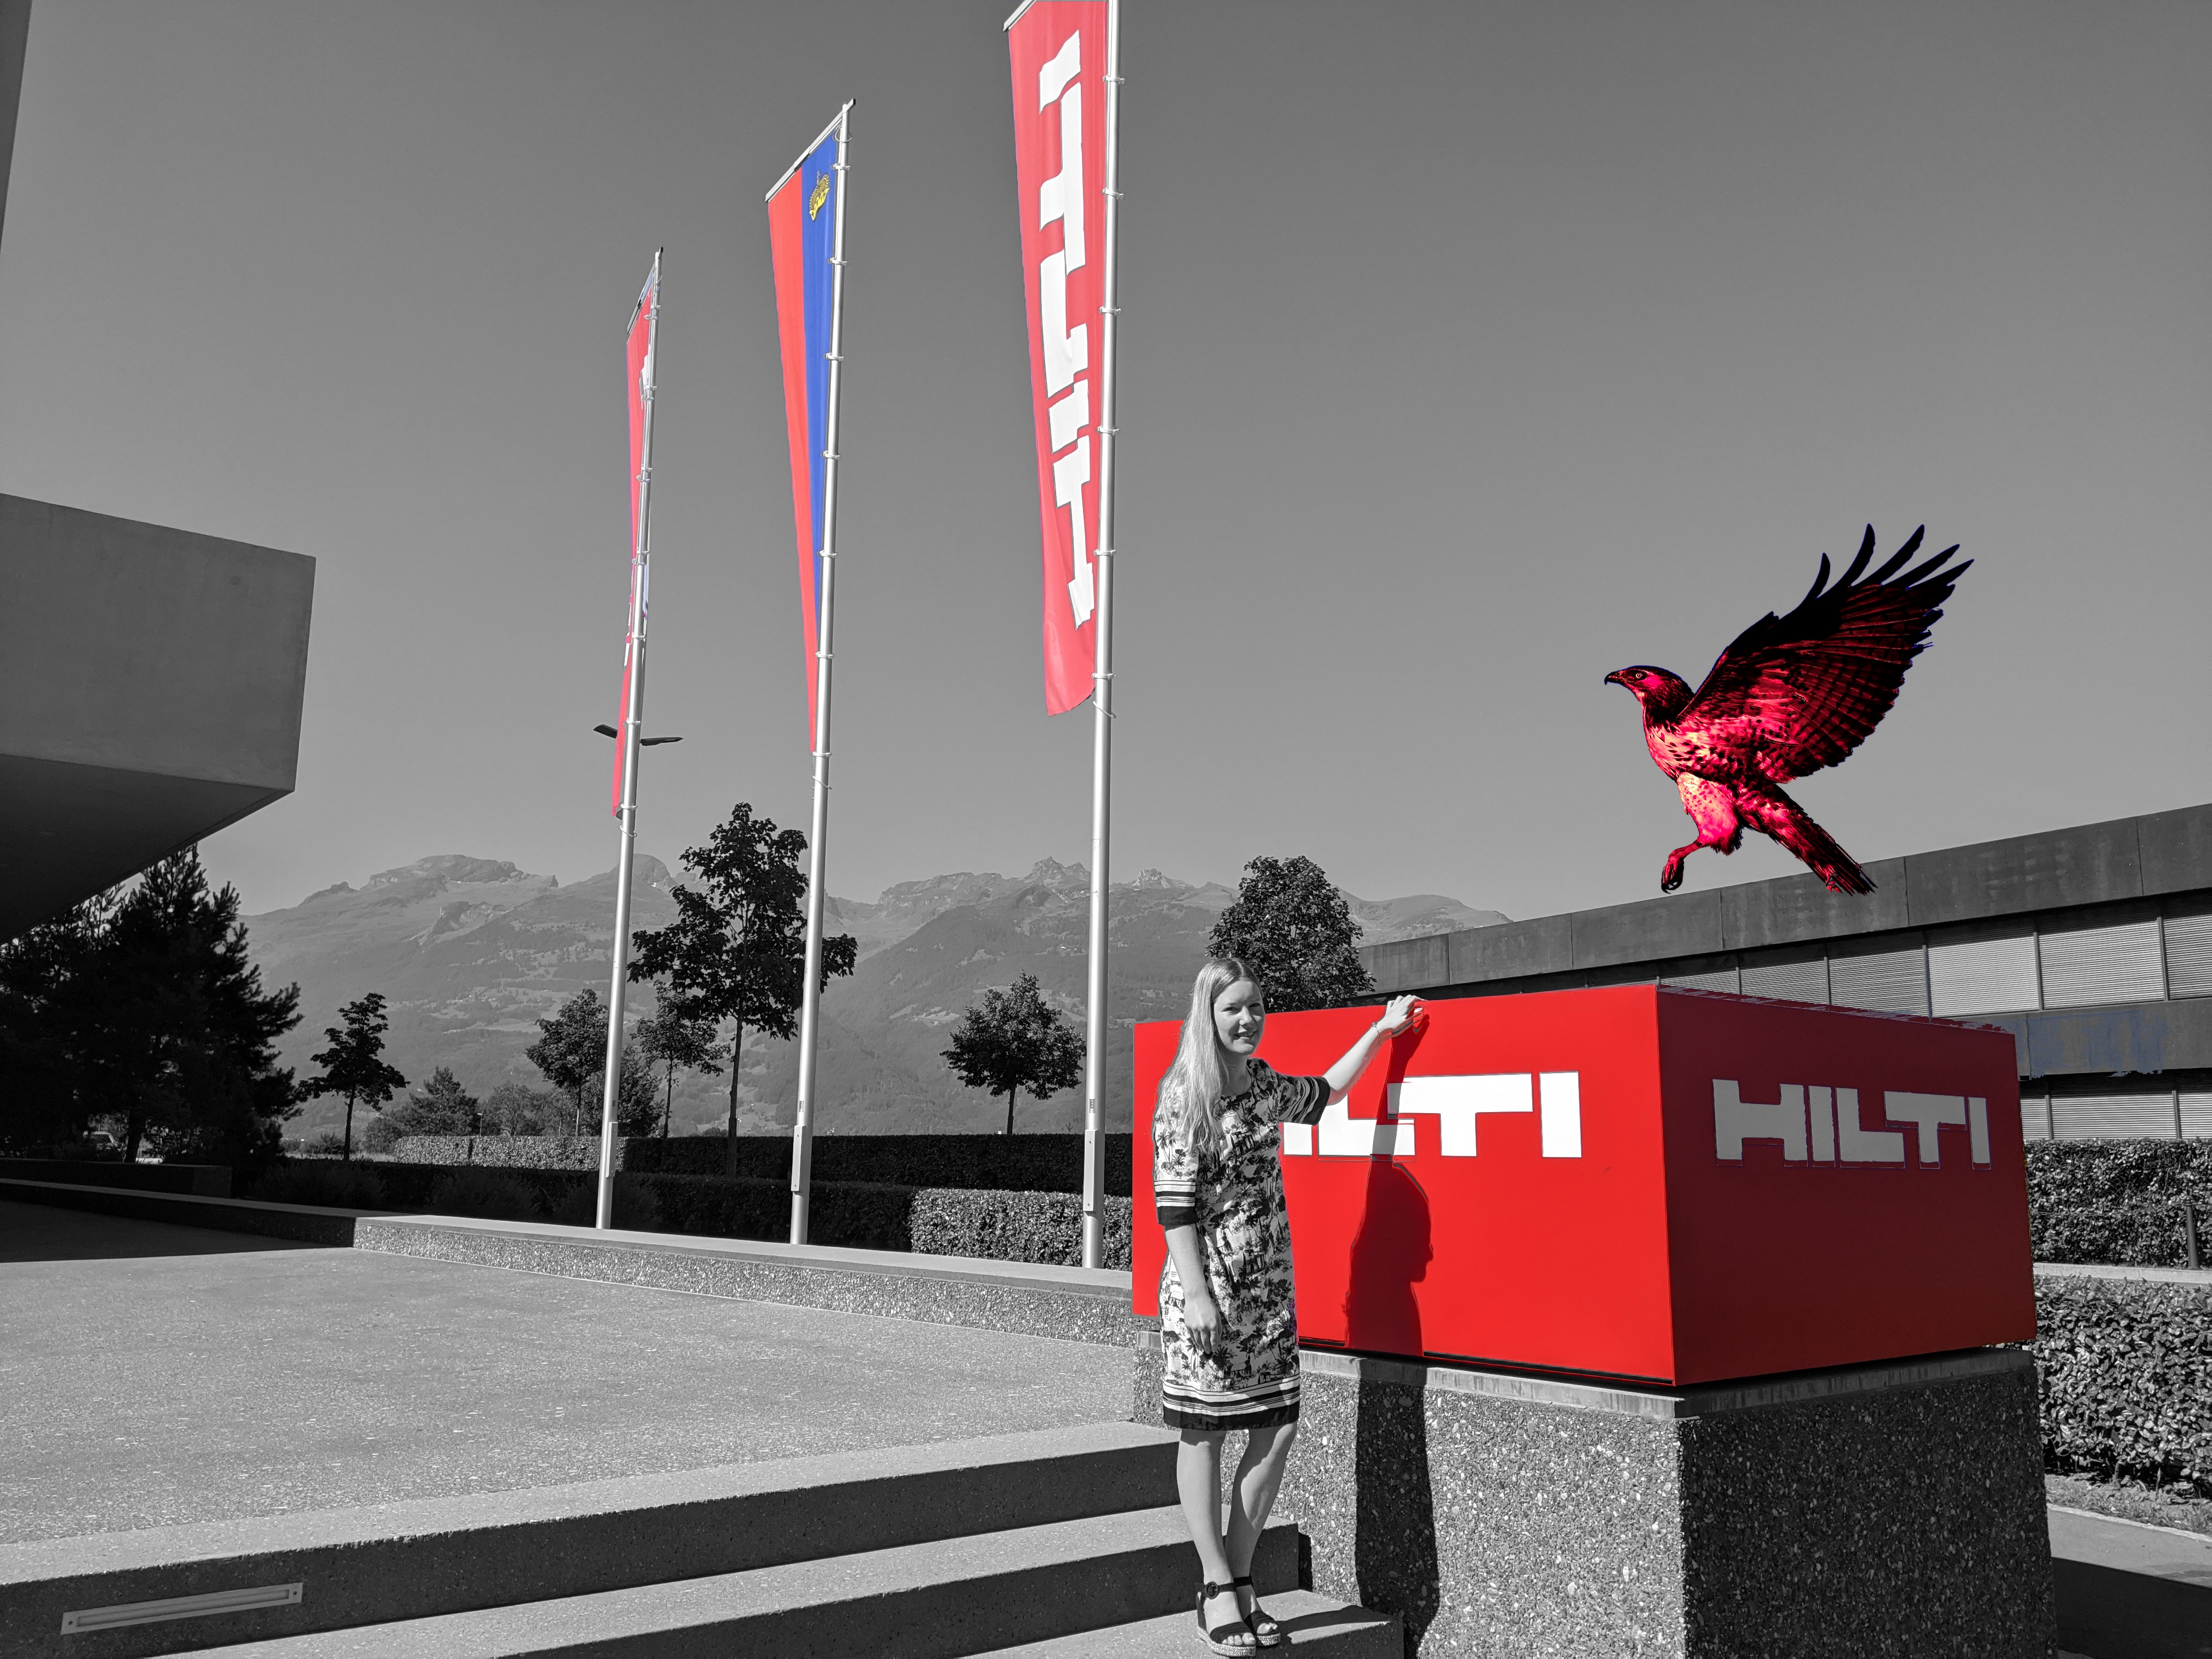
\includegraphics[scale=0.07]{figure/IMgarde.jpg}~\\[1cm]
\end{figure}
 		
\end{center}


\clearpage
		
\newpage

\tableofcontents
\newpage

\thispagestyle{empty} 
    \begin{center}
		{ \huge \bfseries Abstract}\\
		\rule{\linewidth}{0.2 mm} \\[1.5 cm]
    \end{center}
    
  \par The applications of Machine Learning and Computer Vision is rapidly increasing in all field of industry. It has undoubtedly affected the processes of quality assurance. Hilti AG in Schaan, Liechtenstein, is currently aiming at implementing various Machine Learning algorithms, particularly on the production of screws and anchors. Despite manual visual inspections that are carried out, false and unreadable embossments of screws and anchors are not always recognized. The manual quality control differs from worker to worker and from time to time. The losses to the company because of such errors are worth tens of thousands of Swiss Francs. The aim of this work is the development of an image and text recognition application to read and assess automatically the quality of engravings on steel surfaces. Incorrect or defective embossing on screw and anchors should be identified so that the punch can be replaced as soon as possible. To reach this goal we implemented an object detection network grounded on the Faster R-CNN algorithm, which allows reading curved embossing text whatever the orientation of the object. This model has been integrated into a graphical user interface remotely connected to a GPU playing the role of a server, to keep the detection time as short as possible, and offer a user-friendly solution. The solution developed is already working on the production line and we are currently improving the detection of the wear of punches and extending the model to more products.
  

\clearpage
\newpage


%----------------------------------------------------------------------------------------
% Introduction
%----------------------------------------------------------------------------------------
\setcounter{page}{1} % Sets counter of page to 1
%----------------------------------------------------------------------
% Acronym definitions
\newacronym{AI}{AI}{Artificial Intelligence}
\newacronym{BU}{BU}{Business Unit}
\newacronym{CNN}{CNN}{Convolutional Neural Network}
\newacronym{FC}{FC}{Fully connected layer}
\newacronym{NMS}{NMS}{Non Maximal Supression}
\newacronym{R-CNN}{R-CNN}{Region-based CNN}
\newacronym{SVM}{SVM}{Support Vector Machine}
\newacronym{RoI}{RoI}{Region of Interest}
\newacronym{YOLO}{YOLO}{You only look once}
\newacronym{SSD}{SSD}{Single-shot detector}
\newacronym{TP}{TP}{True Positive}
\newacronym{FP}{FP}{False Positive}
\newacronym{FN}{FN}{False Negative}
\newacronym{RPN}{RPN}{Region Proposal network}
\newacronym{mAP}{mAP}{mean Average Precision}
\newacronym{AR}{AR}{Average Recall}
\newacronym{UI}{UI}{User Interface}
\newacronym{IoU}{IoU}{Intersection over Union}
\newacronym{GPU}{GPU}{Graphics Processing Unit}
\newacronym{SGD}{SGD}{stochastic Gradient Descent}
\newacronym{OCR}{OCR}{Optical Character Recognition}
\newacronym{BIM}{BIM}{Building information and modeling}
\newacronym{GUI}{GUI}{Graphical User Interface}
\newacronym{MVC}{MVC}{Model View Controller}
\newacronym{TCP}{TCP}{Transmission Control Protocol)}
\newacronym{IP}{IP}{ Internet Protocol}
\section{Introduction}
\subsection{About Hilti group}
\hspace{24pt} Hilti has been founded in 1941, in Lichtenstein, by Martin Hilti. Since its creation this familial company has became an international leader in the construction industry, with high quality tools and technologies. Today the company counts 30000 employees, whose 15000 in sales force, and 9 plants in Schaan (Lichtenstein - headquarters), Thüringen (Austria), Kaufering and Strass (Germany), Kecskemet (Hungary), Zhanjiang (China), Matamoros (Mexico) and Gujarat (India). The current CEO Christian Loss, introduced the "Champion 2020" corporate strategy. Focusing their strengths on product and services differentiation and a direct customer relationship, this winning strategy will be extended to 2023.
\par Hilti's direct sale model is one of its main strength in front of their competitors. Hilti product are dedicated to professionals, who can buy them directly in Hilti's stores on their website, or by telephone. Their close relationship with construction professional, and their presence on building site, increase their innovation capacities. Like this, the company invest around 6 percent of its turnover each year in research in development, allowing to the company to stay ahead in term of technology. 
\par If Hilti main products remain anchors, installation systems, fire protection installation, power tools, measuring and detection tools, demolition hammers, cordless electrics drill and diamond drills, the company is also diversifying its activity toward services like \gls{BIM} services, or design soft wares. This internship took place in Schaan in a context of the transition toward the industry 4.0, focusing on how the artificial intelligence (\gls{AI}) techniques can be used to increase the quality of the production. 
\subsection{Organization of the headquarters (Hilti Schaan)} 
Customers needs and requirements define the global strategy of the whole company. Customers interact directly with the sale department which gathered around 50\% of Hilti's employees. The information collected by the sale department help to define the objectives of the different business units (\gls{BU}). Hilti's business units are divided in two business areas that are respectively the area of electric tools and accessories and the area of fastening and protection. Each \gls{BU} represents a division of the global company and are respectively responsible of a set of products and services that belong to a specific field of activity. Each \gls{BU} have the duty to define the strategy and to take the operational decisions according to the specific goals and issues of their respective field. The organization and objectives of plans result from these \gls{BU}s' strategies. The production activities in Schaan are divided between diamonds segments, direct fastening element and metal anchors. The productions lines are coordinated and supported by the control, the quality, the lean and the tools\footnote{The tools unit produces the elements needed to the production of the final products.} units. This internship has been realized within the quality team which will be introduce in following section. Customers' expectations and \gls{BU}s' strategies define the research and development (R\&D) goals. The budget annully allocated to R\&D is investin at 30\% in long term differentiation projects and respectively 50\% and 20\% in mid and short term projects. The production is supported by different department and especially by the logistic department. Finally, the organization relies on global department such as information and technology, human ressources, intellectual property [\textcolor{red}{Fig.}\ref{fig1_Hilti_organization}]... 


\subsection{Presentation of the quality team}
The activities of quality team are under the direction of the global manufacturing department lead by Armin Kueper. Seppo Paraemaeki, the head of the quality, leads a team of 22 people, whose my supervisors Unger Stefan (Quality manager) and Koch Julian (Quality specialist). 


%-----------------------------------------------------------------------------------
\subsection{Introduction to the case study}
Machine learning and artificial intelligence techniques are catching more and more attention in various fields of application (industrial, medical...). Presently they can be seen above all in the networking of machines and the emergence of novel technology and systems that can significantly increase productivity, efficiency, and quality within production. These methods include predictive maintenance solutions, independent manufacturing processes, or automated quality controls. Especially, deep learning models can be used to support manual visual inspection tasks. For some authors, these systems outperform a higher defect rate than comparable inspection performed by humans \cite{cha2018autonomous}. Following these inclinations, the research paper within the Smart Factory Initiative of Hilti AG focused on the development of a visual inspection system that can be used for screws and anchors. Therefore, the general aim of this internship is the implementation of a system able to read and assess the quality of the engraving text on steel surfaces. This case of study can be only partially solved through commercial \gls{OCR}s services \cite{AzureOCR, AWSOCR, GoogleOCR}, because of engravings' circular shape. Our research has, therefore, be focused on the following questions:
\begin{enumerate}
\itemsep0em 
    \item In which sub-cases commercial \gls{OCR} software, which is the quickest solution in terms of implementation and the easiest and cheapest in terms of maintenance, can be used? This interrogation led us to question which is the best commercial service for our case study.
    \item Since these commercial \gls{OCR}s services are not efficient in reading curved texts, we have focused our attention on object detection techniques \cite{girshick2015fast}. Then the central question of this study is: which is the object detection technique allowing reaching the best accuracy, without in the first time any speed constrain \cite{girshick2015region, ren2015faster, redmon2016you, liu2008robust}? The training of an object detection network with the objective to reach 98\% of fully correctly annotated pictures in the test set brought a lot of challenges. Firstly, the training set has to be enough wide to cover most of the cases and especially different object orientations. The size of the training set led us to think about a semi-supervised labeling process, to shorten the labeling process extremely time-consuming. Secondly, the performances obtained in the laboratory have to been transposable on the production line, and therefore a strict and reproducible framework had to be defined.
    \item Finally, since the solution has to help the workers in their daily tasks, we have to think about an application user-friendly in terms of use and speed. These led us to question ourselves about the best software architecture guaranteeing both stability and speed.
\end{enumerate}
This report aims to answer these questions, that is why we first developed a methodological section that described in detail the study case and its challenges, the global functioning of commercial \gls{OCR} services, and object detection techniques. We established in this goal a review of the existing object detection algorithms, focusing our analysis on Faster-\gls{R-CNN} \cite{ren2015faster}, the solution finally chosen. This section also gathers the different steps that allowed the setting up of this model, namely the composition of the data set and a description of the labeling process, the descriptions of the soft-wares and hard-wares environments, the optimization algorithm chosen, and the metrics that allowed to assess the performances of the models. Finally, this section describes how we implemented a user-orientated solution with a description of the protocol comparing the expected label to the predicted one and a description of the \gls{GUI} architecture. The results section firstly presents a comparison between three commercial \gls{OCR} services, tested on a benchmark data set relative to our study case, to explain our choice to work with Azure solution \cite{AzureOCR}. Secondly, it presents the performances of our object detection algorithm, with a comparison between two feature network  \gls{CNN} tested with the Faster-\gls{R-CNN} model. Finally, the results section included a detailed description of the user's interface and of the underlying client/server architecture. These results allowed us to open a discussion on users' feedbacks and on the following objectives this case study, especially, on how to extend the existing solution to others products, and how to improve the detection of the wear of stamps.



%-----------------------------------------------------------------------------------
\section{Materials and methods}
\subsection{Description of the case study}
We worked on the quality control of screw [\textcolor{red}{Fig.}\ref{quality_cylce_main}\textcolor{red}{-B}] and anchors labeling [\textcolor{red}{Fig.}\ref{quality_cylce_main}\textcolor{red}{-C}], in the following section will used a model named quality control cycle to describe the problem [\textcolor{red}{Fig.}\ref{quality_cylce_main}\textcolor{red}{-A}]. This model based on technical control circuit aims at creating a product with a predetermine quality \cite{linss2018qualitatsmanagement}. Therefore, quality control cycles consist of an execution of an activity, the analysis of the resulting quality according to measurable characteristics values and a possible triggering of corrective actions. We call $x$ the control variable, that refers to the generated quality of the product, in our case the quality of screws and anchors labeling. $x$ should be a constant whose the value is as close as possible of $w$ the reference variable that defines the quality requirements. the differences between $x$ and $w$ is called the deviation $e$, these deviations occur mainly for two raisons:
\begin{enumerate}
\itemsep0em 
 \item the wrong stamp has been used;
\item The wear of the stamp during the production led in quality deterioration of the characters punched.
\end{enumerate}
The first case leads to losses of several thousand Swiss francs the past years. During production planning, care is taken to ensure that similar anchors and screws are produced after the other so that the set up time is kept as short as possible. Nevertheless, these products have similar designations what increases the risk to use the wrong stamp. This case can be also explained by the fact that stamps show a mirror inverted profile that complicates the reading [\textcolor{red}{Fig.}\ref{quality_cylce_main}\textcolor{red}{-C}]. The second case affects predominantly characters with closed forms such as 0, 8 or 9, because during the embossing the material inside the closed areas cannot spread outwards and thus pressed against the punch. These hazards $z$ at the origin of $e$ have to been captures by a measuring element. A first control element evaluate and interpreter information given by the measuring system and returns the manipulate variable $y$. $y$ becomes the input of the controller that initiates measures and guarantee their implementation before to feed back the control system [\textcolor{red}{Fig.}\ref{quality_cylce_main}\textcolor{red}{-A}]. The current quality control cycle is grounded on visual control, therefore the measuring element is the employees' eyes. Workers, as the first control element, compare the quality of the produced label to the expected one. As described, this crucial comparison is subject to failures, that is why it has been asked to the employees to copy down the embossing during the visual inspection and to have it compare by a second worker [\textcolor{red}{Fig.}\ref{quality_cycle_sup}\textcolor{red}{-A}]. Despite of this precaution, expansive errors remain, that is why we will propose a quality control cycle grounded on computer vision techniques. The measuring element becomes a camera, and the first control element a neural network or a \gls{OCR} software, predicting the characters on pictures. The return variables of these algorithms are probabilities reflecting the degree of confidence in the prediction for each character. The characters associated to high probabilities are used to generated a string (the predicted label), which is compared to the expected one [\textcolor{red}{Fig.}\ref{quality_cycle_sup}\textcolor{red}{-B}]. In these two cycles the only measures sufficient to restart the production are to clear or replace the stamp [\textcolor{red}{Fig.}\ref{quality_cycle_sup}].\\
Our case study is focused on two types of embossing with linear and curved cases. For the linear engraving that are used for anchors, labeling are directly read through an existing \gls{OCR} service. If this solution is fast to implement and easy to maintain, it has proven to be not been able to read curved text, that is why for screw labels we implemented our own object detection network. In this case study several challenges have to be taken into account. Firstly, picture quality should be constant and as closed as possible than the one used to trained the network. Thus, despite of varying lightning condition in the production line, objects should be constantly illuminated to get rid of the potential reflections induced by the steel surface. Secondly, algorithms response time have to be kept as low as possible to encourage the use of the new solution. Thirdly, the solution have to be compatible with company policies and therefore develop under Microsoft environment. Fourthly, it should be easily generalizable for other type of anchors and screws produced on other plants.

 \begin{figure}[H]
 \centering
 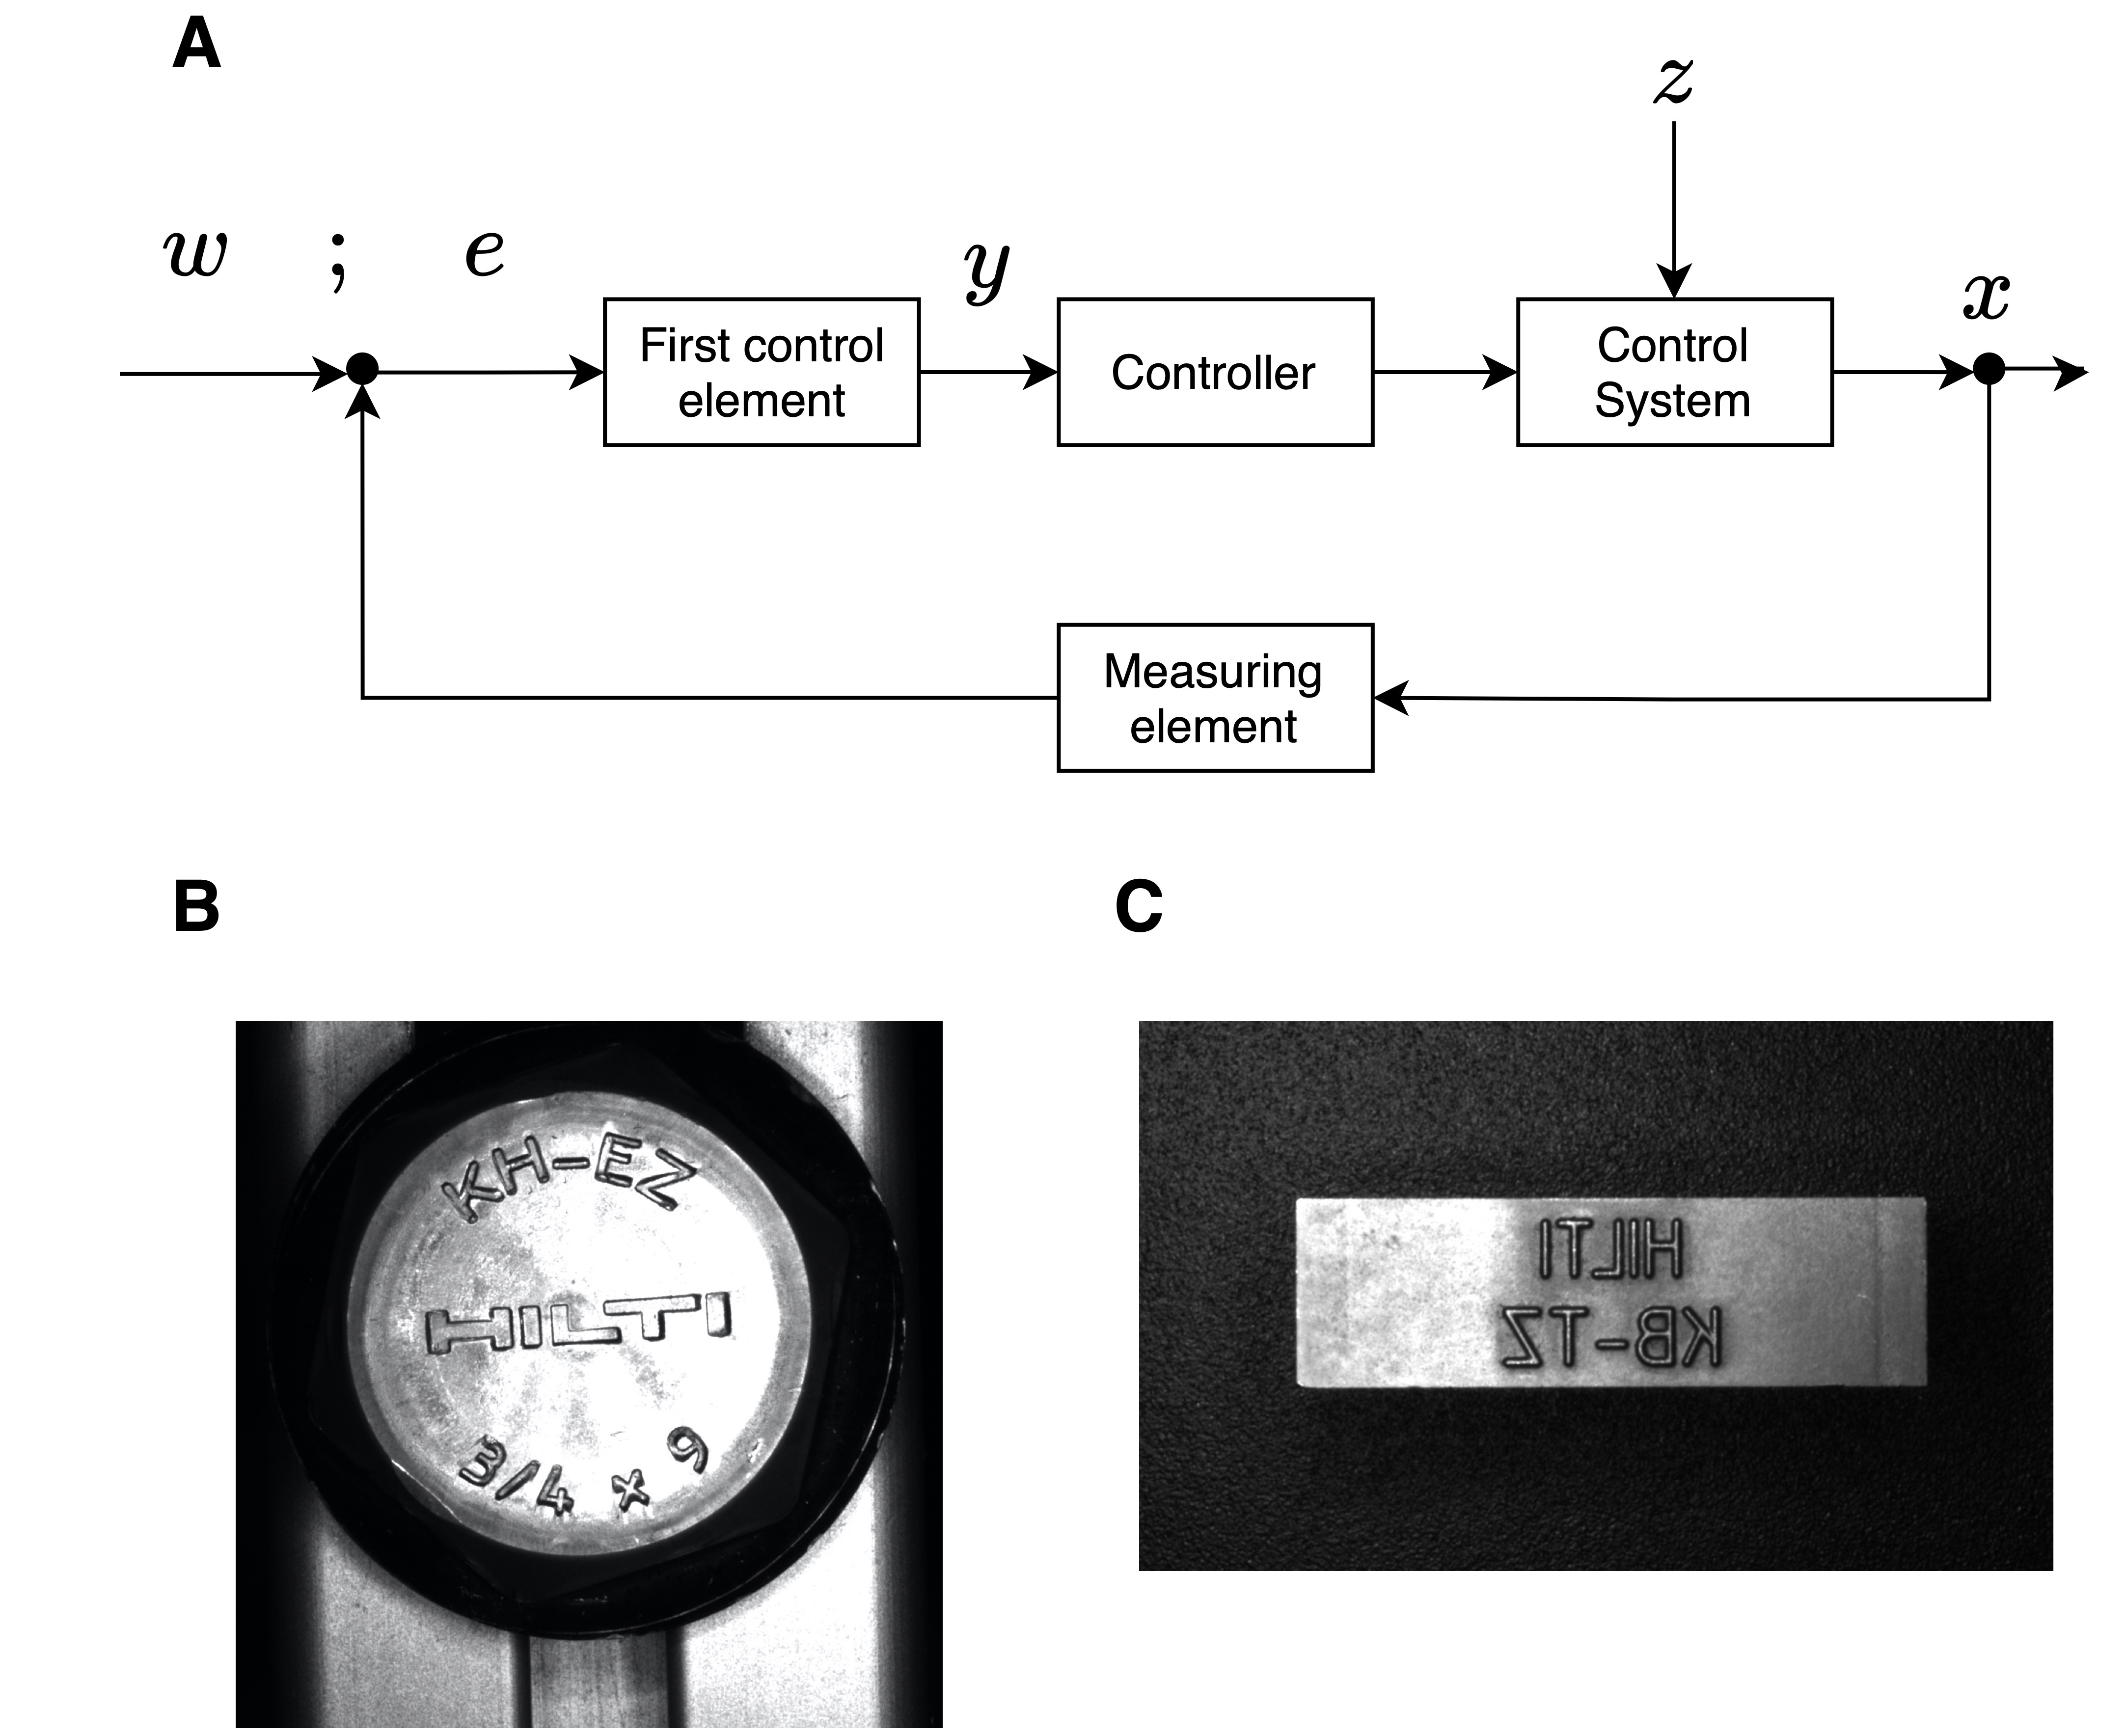
\includegraphics[width=0.7\textwidth]{figure/quality_cycle_main.jpg}
 \caption{\textbf{Presentation of the problematic.} \textbf{A)} Quality control cycle diagram \cite{linss2018qualitatsmanagement}.\textbf{B)} Typical picture of screw. \textbf{C)} Typical picture of stamp for anchor labeling. }
 \label{quality_cylce_main}
\end{figure} 

\subsection{Optical Character Recognition overview}
\gls{OCR} algorithms work in mainly three steps \cite{zhang2013text}:
\begin{enumerate}
\itemsep0em 
 \item localization and detection of the text,
 \item enhancement and segmentation of the character,
 \item classify the detected characters.
\end{enumerate}
Mainly three approaches are used to realize the first step, which is crucial for text detection in natural scenes. It can be done by edges detection methods that apply mainly canny filters and morphological operations to extract text area. Nevertheless, these techniques are sensitive to shadow or highlighting, and to complex backgrounds. The second approach consists of texture analysis through Gaussian filters, Fourier transformation, or local binary pattern analysis. The extracted regions are then used to feed a binary classifier grounded on a neural network or on a different heuristic to discriminate text and non-text areas. The third technique is based on connected-component based methods \cite{liu2008robust}. Firstly the picture is binarized and the smallest and largest components (\textit{ie} regions in the binary picture) are deleted. Then, neighboring components sharing a similar intensity histogram are merge based on the assumption that text components shared more similar intensity histograms than non-text components. Finally, to prune non-text area shape filters are used. Assuming that text components are composed of different characters the affinity within a component can be measured through the standard deviation between the inner distance between all pixels in a component. Components with an affinity lower than a given threshold are classified as background and remove \cite{liu2008robust}. This last technique is often more accurate than the others since it focuses on local and detailed pixels analysis \cite{zhang2013text}. The second step consists of text enhancement and segmentation. One of the major steps is picture binarization, where finding the right threshold is a problem on its own. Different methods can be applied such as dichotomic binarization per region defining themselves by pixels intensity, or adaptative thresholding methods based on texture analysis \cite{zhang2013text}. Then, text orientation should be corrected, and so pictures' skew angle has to be calculated. Several techniques are commonly used such as the projection profile. Assuming that a based line is mainly defined by black pixels, vertical and horizontal lines are projected to get the sum of the black pixels that they overlap. The image is rotated to by one degree the sum is recalculated if it is higher than the current one, the score is updated. After repeating the operation until rotation of $90\degree$, the maximal score can be associated with picture's skew angle. Another approach searching the nearest neighbors of each character and computing the histogram of these values can be also used to determine the skew angle \cite{parashar2012finding}. Text enhancement also consists of image despeckle, applying different filters such as Gaussian and blur filters. Finally, the text is decomposed into lines, lines into words, and words into characters during a process called segmentation. This is done by firstly detected on the binary picture the height and the width of the lines through an analysis of the gap in the binary histogram. Then, the process is repeated for words and then characters. The final step involves feeding a neural network trained to classify characters with the bounding boxes isolating the presumed characters. This last step can be also realized through a matching profile technique, but it has been progressively left for neural networks to deal with more various font sizes. \gls{OCR} services are often efficient on scanned documents, but extracting text in natural scenes is a highly more challenging problem since software has to deal with, various font size, different text orientation and alignment, potential distortions resulting from camera angle and perspective, or weak edges between the text and the background \cite{zhang2013text}. In this case study, we compared three commercial \gls{OCR} services: Google OCR \cite{GoogleOCR}, Azure OCR \cite{AzureOCR}, and AWS OCR \cite{AWSOCR}. Their performances have been respectively assessed on linear stamp and screws cases \footnote{This section explains the general functioning of OCR services since, the technical details of the commercial soft wares compared are not available.}.
 


\subsection{Object detection: state-of-the-art}
\newacronym{bnd box}{bnd box}{bounding boxes}
Convolutional neural networks (\gls{CNN}) are the most used and the most preferment systems for object detection. Object detection is a computer vision problematic consisting in determining the position and the class of each object in a picture. A naive approach would involve segmenting a picture in windows to feed vanilla classifier that would predict for each fragment the presence or absence of an object and its potential class. This time consuming approach implies that the size of the different objects is known and constant \cite{michelucci2019advanced}. Since in many cases this assumption cannot be made, most of the object detection methods propose adaptive size bounding boxes to surround proposals. In the following section, we will present the state-of-the-art of object detection techniques and then describe into detail the most accurate one Faster \gls{R-CNN}. 



Object detection techniques based on \gls{CNN}, introduced with the \gls{R-CNN} algorithm, for Region proposals with \gls{CNN}\cite{girshick2015region}, mark a turning point in this field of study. \gls{R-CNN} uses a selective search algorithm to extract regions of interest (\gls{RoI}), that potentially contain objects [\textcolor{red}{Fig.}\ref{fig:art_rcnn}\textcolor{red}]. In order to do so, a selective search algorithm segments images based on pixels' texture and colors similarity [\textcolor{red}{Fig.}\ref{fig:art_rcnn}\textcolor{red}{-step 2}]. Then the regions sharing the same features are agglomerated to create larger areas according to regions' size and shapes compatibility \cite{uijlings2013selective}. After resizing the resultant region proposals, these are successively used to feed a \gls{CNN} from which fixed-length feature vectors are extracted [\textcolor{red}{Fig.}\ref{fig:art_rcnn}\textcolor{red}{-steps 3-4} ]. Then, for a given picture the resulting feature vectors are given as input to different linear support vector machine (SVM) models, trained individually to classified the different classes of objects [\textcolor{red}{Fig.}\ref{fig:art_rcnn}\textcolor{red}{-step 5}]. Finally, a linear regression model is used to adjust the coordinate of the predicted bounding boxes [\textcolor{red}{Fig.}\ref{fig:art_rcnn}\textcolor{red}{-step 5'}].
\par The author of \gls{R-CNN} developed a second version of their algorithm named fast \gls{R-CNN} which allows a reduction of the computation time \cite{girshick2015fast} [\textcolor{red}{Fig.}\ref{fig:art_fast_rcnn}\textcolor{red}]. A deep CNN, such as VGG, takes as input the entire image and creates as output a feature map [\textcolor{red}{Fig.}\ref{fig:art_fast_rcnn}\textcolor{red}{-step 2}]. The regions of interest (RoIs), extracted through the same selective search algorithm as previously described \cite{uijlings2013selective} [\textcolor{red}{Fig.}\ref{fig:art_fast_rcnn}\textcolor{red}{-step 1'}], are projected on these features map. After resizing each \gls{RoI} through a max-pooling layer [\textcolor{red}{Fig.}\ref{fig:art_fast_rcnn}\textcolor{red}{-step 3}], they are successively used as input for fully connected layers (\gls{FC}) [\textcolor{red}{Fig.}\ref{fig:art_fast_rcnn}\textcolor{red}{-step 4}]. The network has two outputs, a FC layer with firstly a softmax activation function that return the probabilities for an object to belong to each class [\textcolor{red}{Fig.}\ref{fig:art_fast_rcnn}\textcolor{red}{-step 5}], and secondly category-specific bounding boxes regressors [\textcolor{red}{Fig.}\ref{fig:art_fast_rcnn}\textcolor{red}{-step 5'}]. The better performances of Fast \gls{R-CNN} can be explained by the fact of that instead feeding a \gls{CNN} successively with the different proposals, the deep \gls{CNN} is trained on the full picture to generate a feature map \cite{ren2015faster}.
\par Faster \gls{R-CNN} is the lastest version of regions based on CNN techniques, which is also the fastest [\textcolor{red}{Fig.}\ref{fig:art_faster_rcnn}] \cite{ren2015faster}. As Fast-\gls{R-CNN} Faster \gls{R-CNN} used a deep \gls{CNN} to generate a feature map. However, instead of using the greedy selective search algorithm to generate RoIs, Faster \gls{R-CNN} is composed of a second CNN, called region proposals network. The detailed architecture of Faster \gls{R-CNN} will be detailed in the following section.
\par Finally, two other methods names respectively \gls{YOLO} [\textcolor{red}{Fig.}\ref{fig:art_yolo}], for You Only Look Once \cite{redmon2016you}, and \gls{SSD} [\textcolor{red}{Fig.}\ref{art_ssd}], for Single-shot detector \cite{liu2016SSD}, don't use region proposals but a single feed-forward convolutional network. Both \gls{YOLO} and \gls{SSD} segment an input picture into a grid of size $S\times S$, and for each cell B predictions corresponding to B different size and scale predefined bounding boxes, also named anchors are made. Each prediction gathers the probability that the box contains an object and its coordinates defined with 4 values $x$, $y$, $w$, and $h$, where $x$ and $y$ correspond to the center of the box and $w$ and $h$ correspond respectively to its width and its height. Like this, a model trained on $N_c$ classes has an output size of $S\times S(B\times 5 + N_c)$. The main difference between \gls{YOLO} and \gls{SSD} is that \gls{YOLO} uses two \gls{FC} layers after the main CNN [\textcolor{red}{Fig.}\ref{fig:art_yolo}\textcolor{red}{-E Step 3}], whereas \gls{SSD} uses various feature maps resulting from different convolutional layers of the main CNN [\textcolor{red}{Fig.}\ref{art_ssd}\textcolor{red}{-step 3-3'-3''}] to generate the final predictions. \gls{YOLO} is most accurate than \gls{SSD} which is faster \cite{huang2017speed}. Although these two models are faster than the region-based methods they are less accurate \cite{huang2017speed}, which is why we didn't explore them to focus our attention on Faster \gls{R-CNN} \cite{ren2015faster}.



% \begin{figure*}[H]
% \centering
% \subfloat[~subcaption1]{\includegraphics[height=6cm, keepratio]{figure/rcnn}}\,
% \subfloat[~subcaption2]{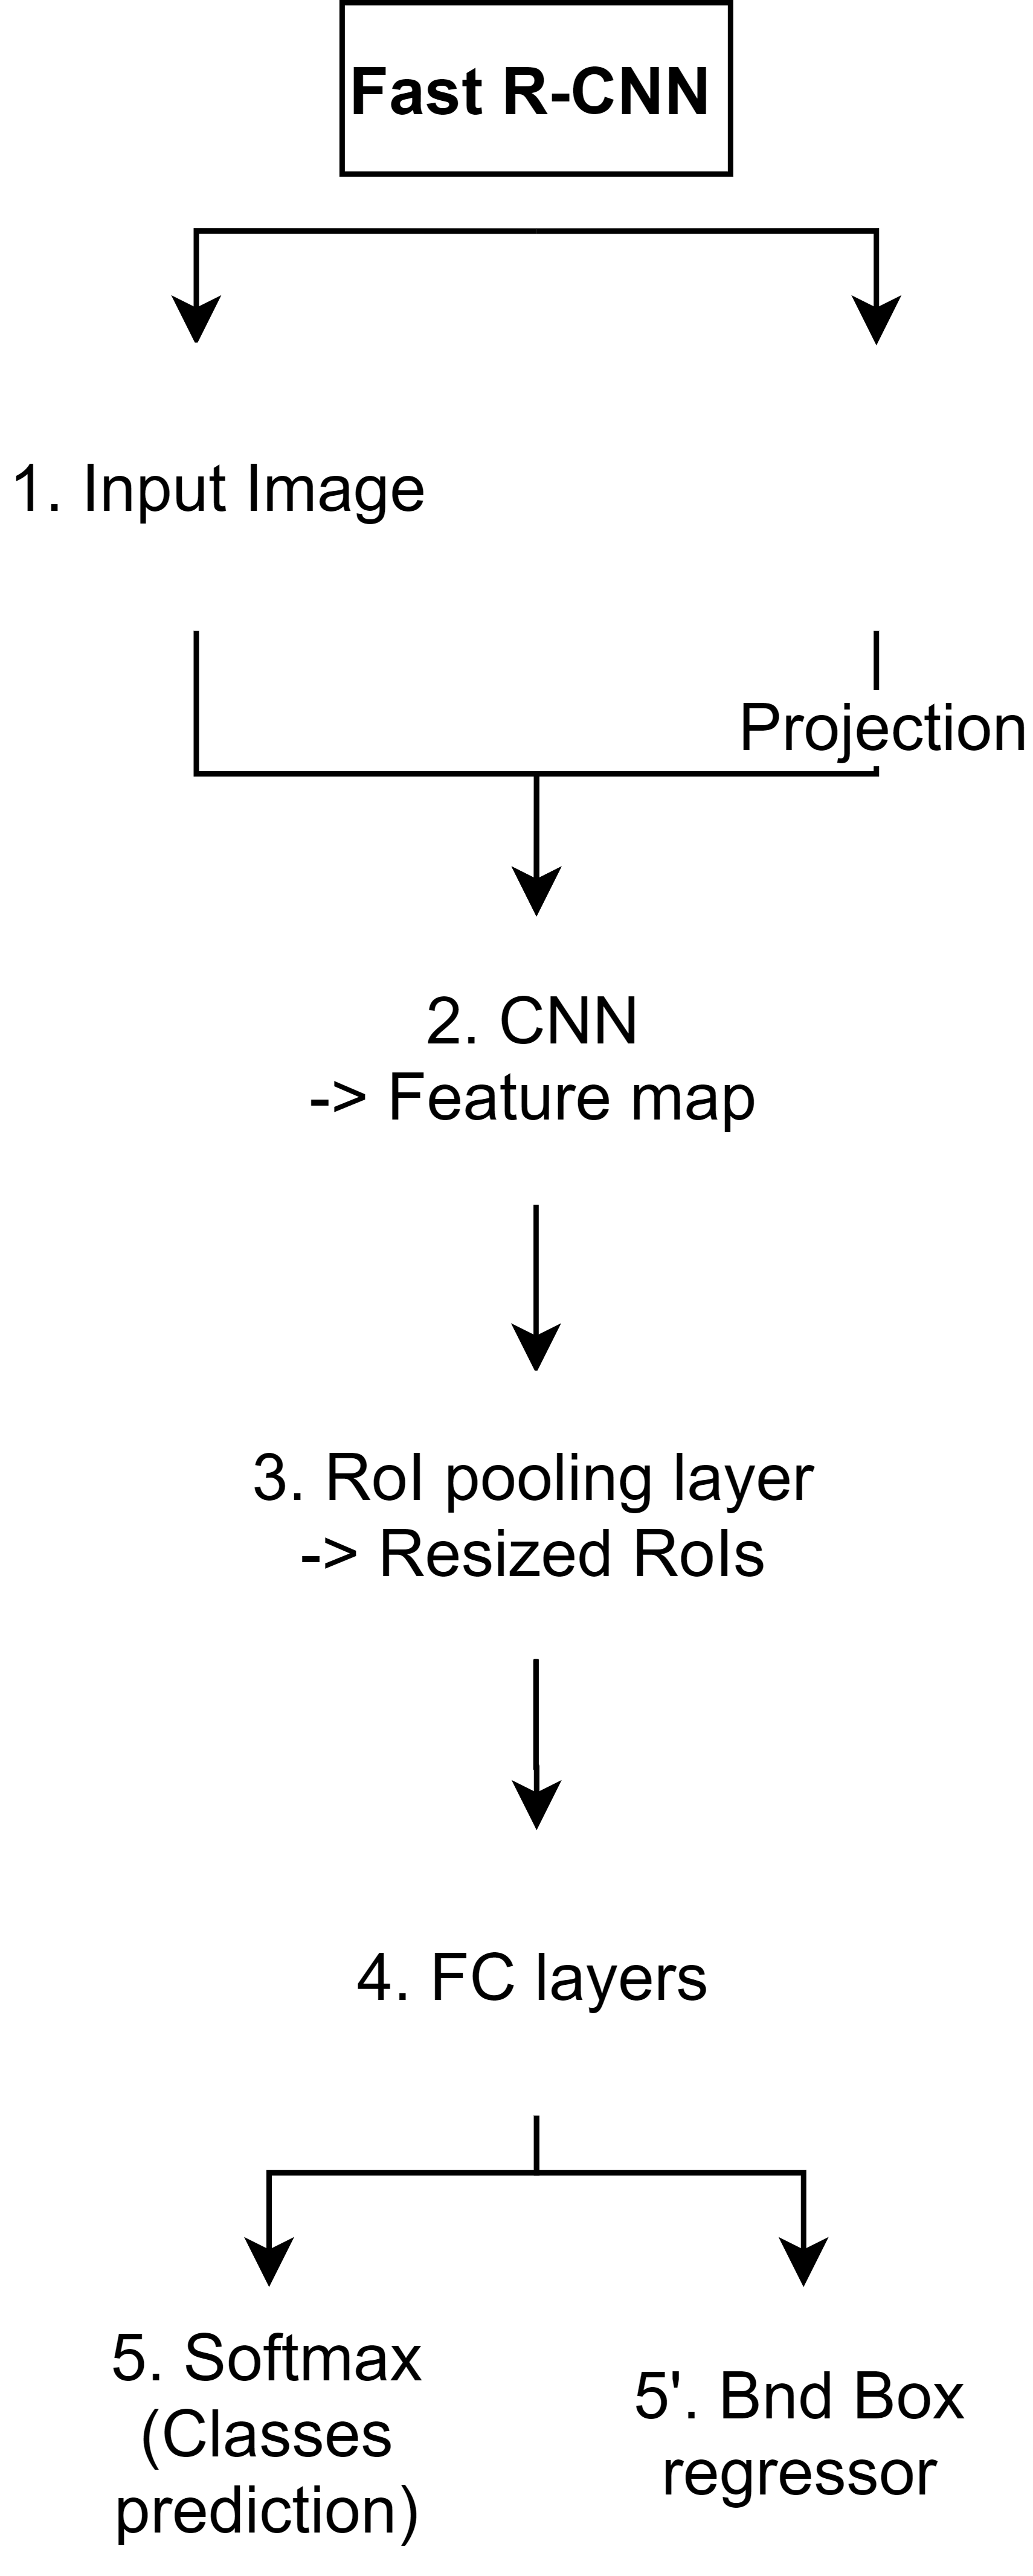
\includegraphics[height=6cm, keepratio]{figure/fast_Rcnn.png}}
% \\
% \subfloat[~subcaption1]{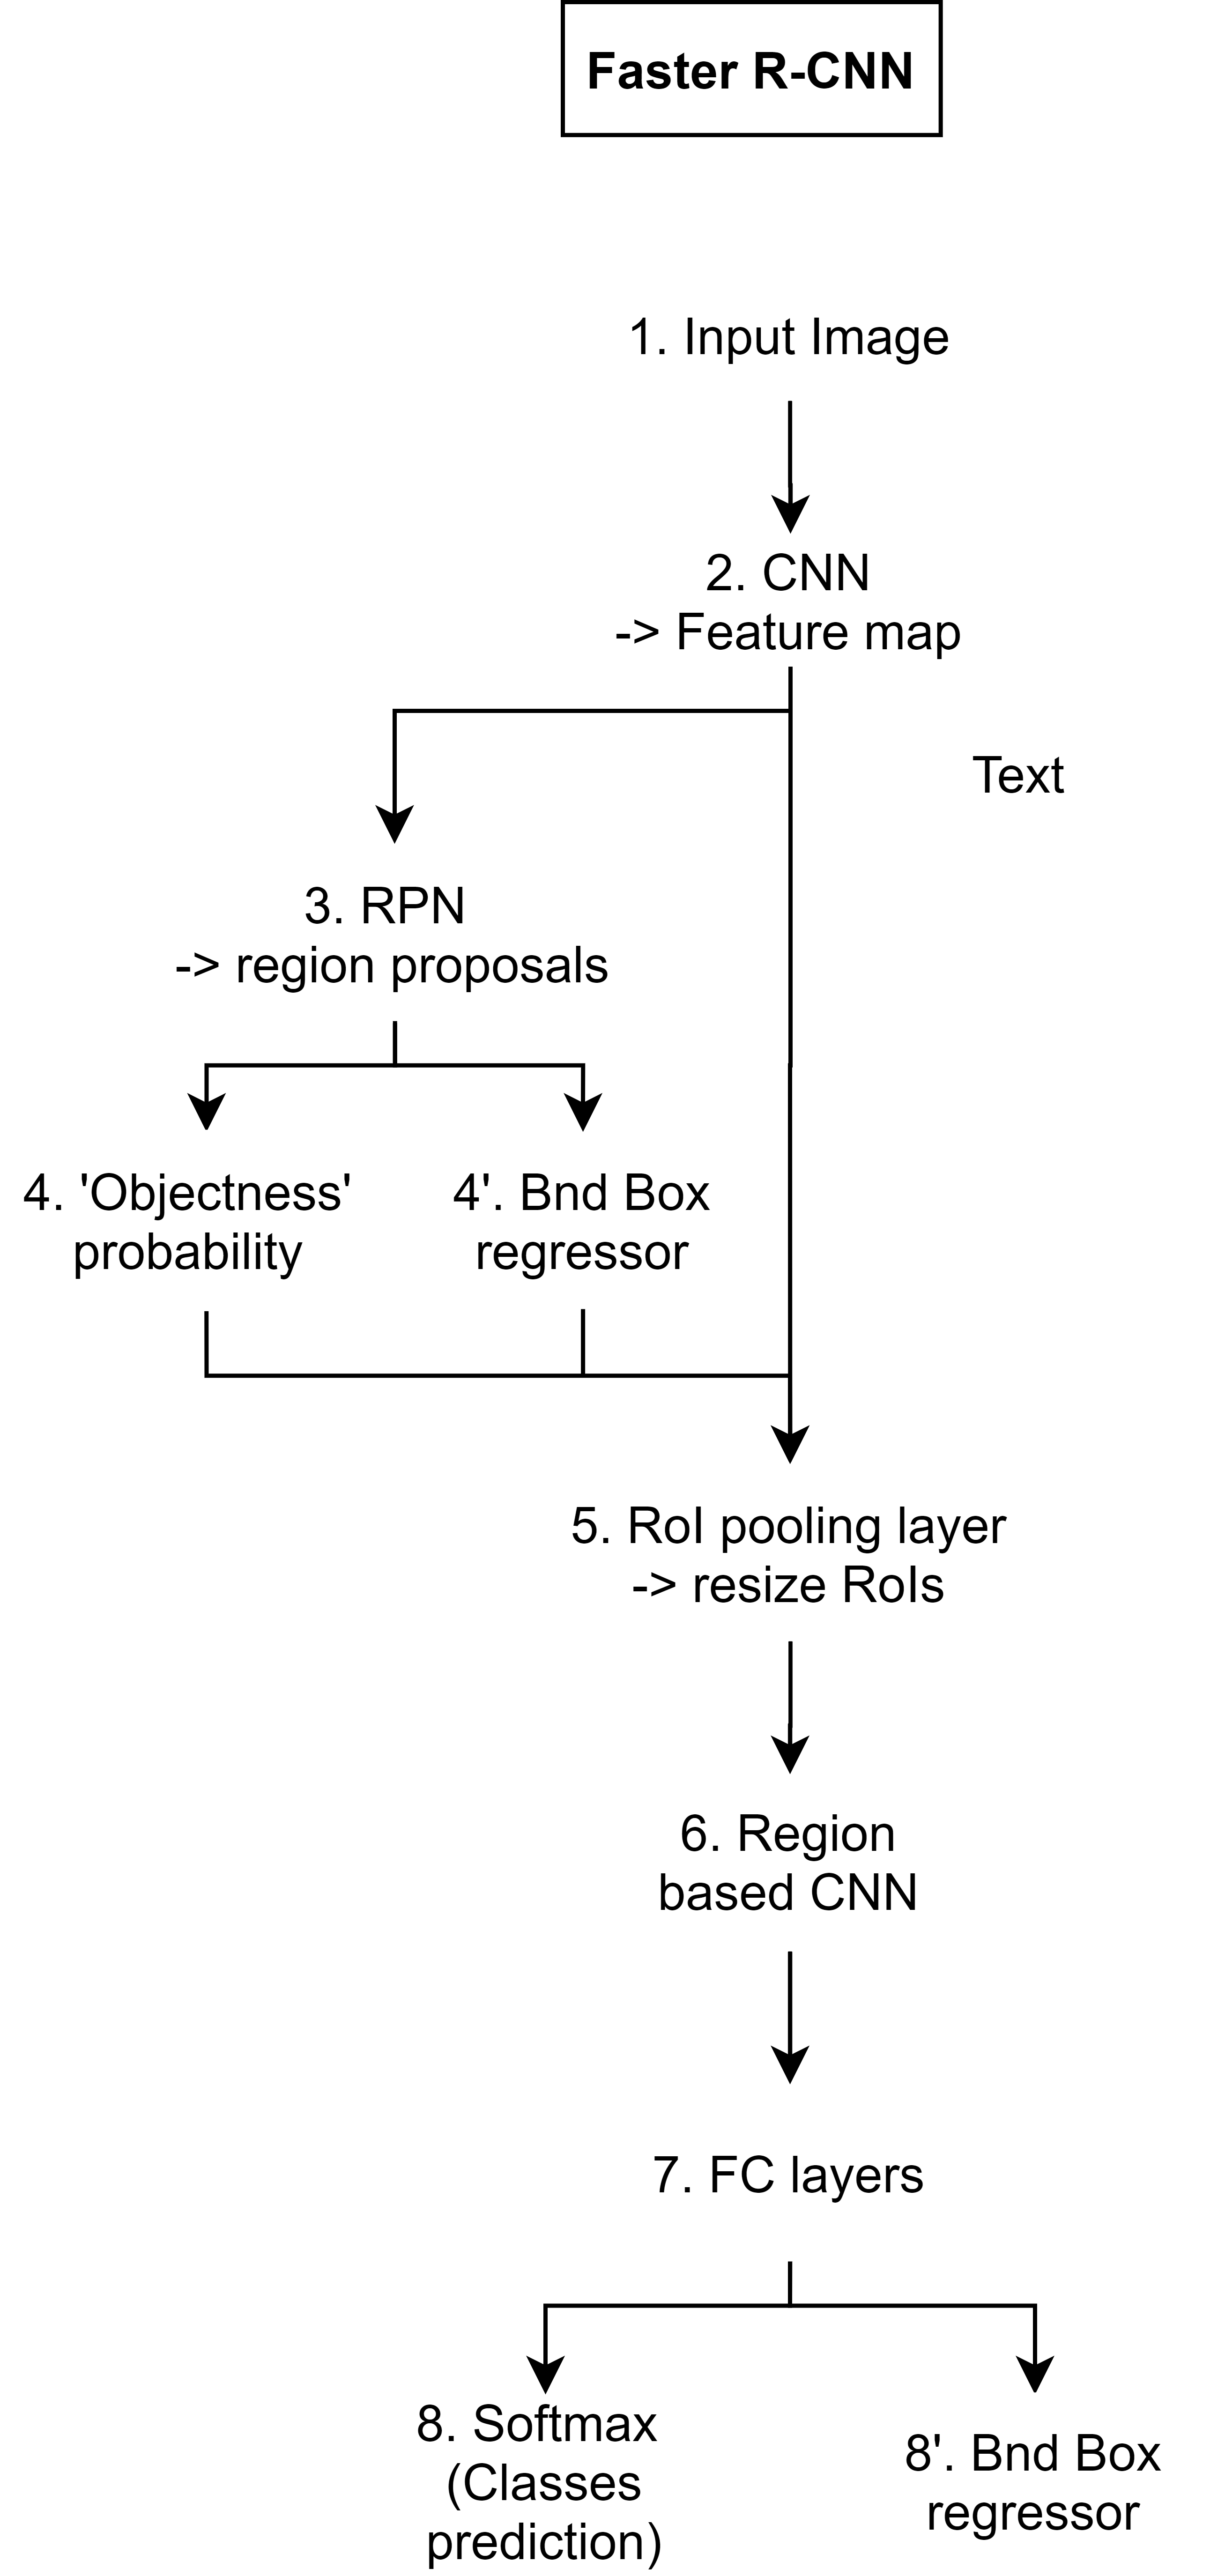
\includegraphics[height=6cm, keepratio]{figure/faster_RCNN.png}}\,
% \subfloat[~subcaption2]{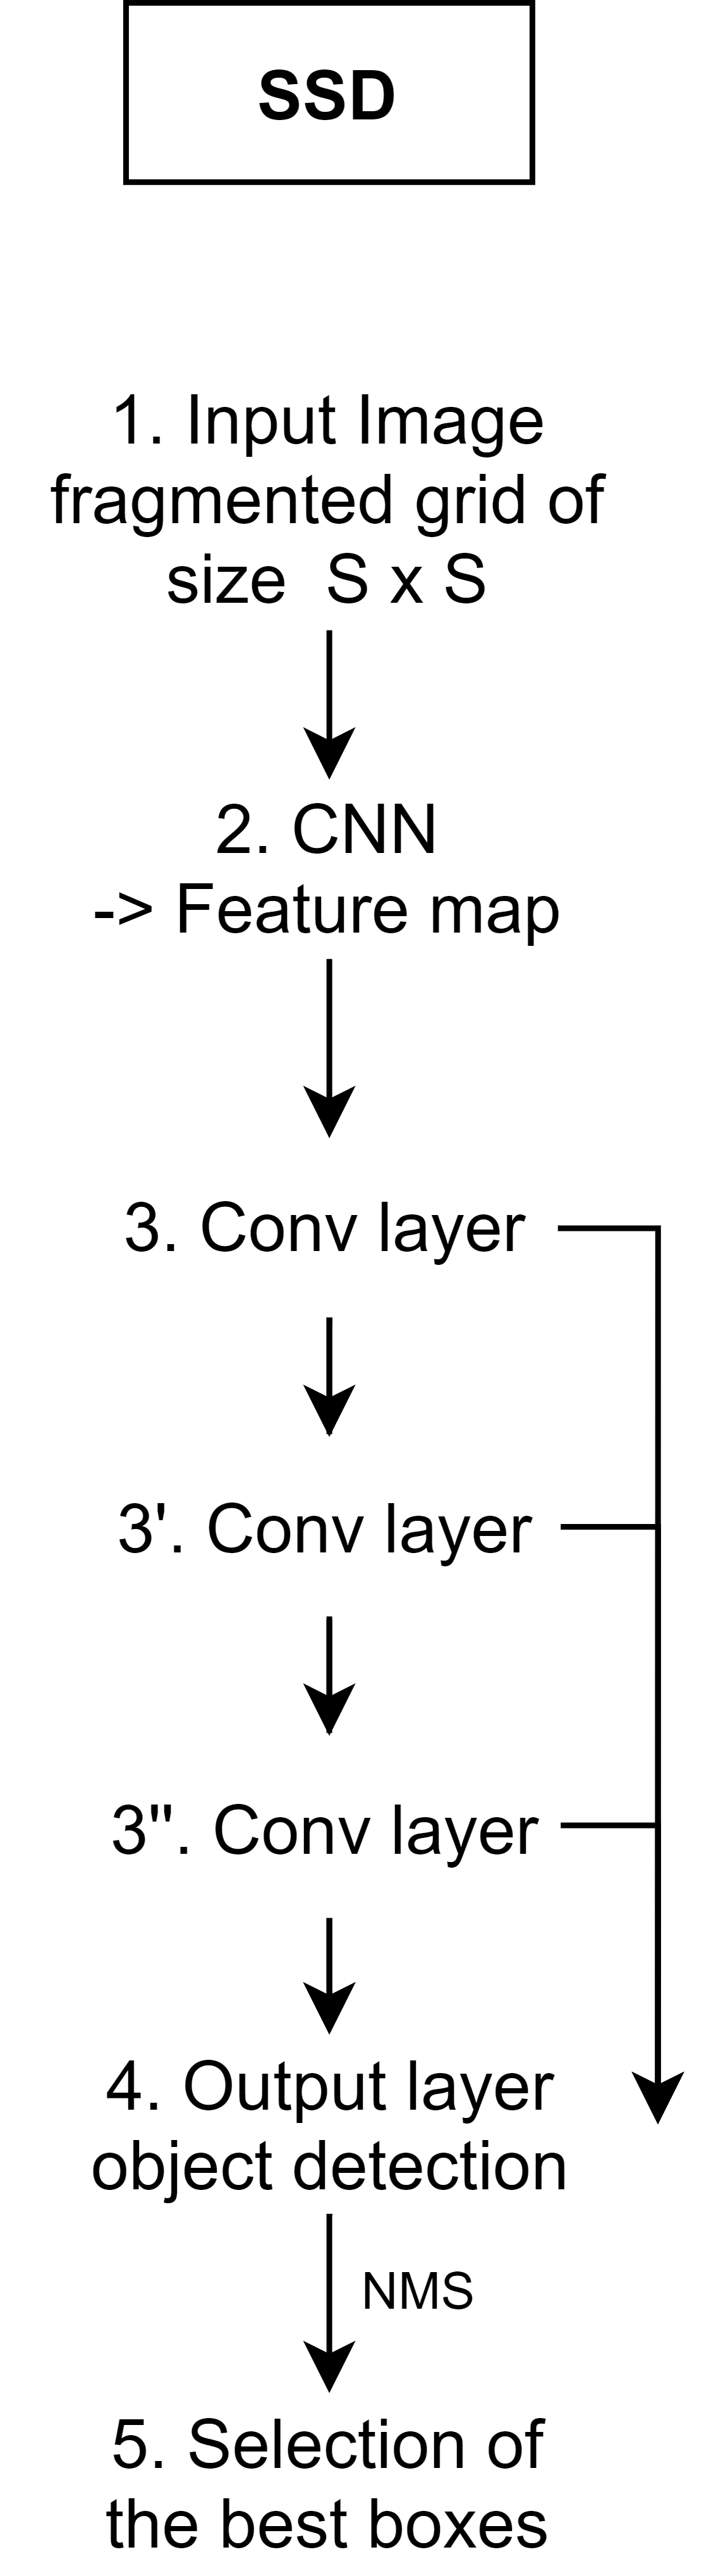
\includegraphics[height=6cm, keepratio]{figure/SSD.png}}\,
% \subfloat[~subcaption2]{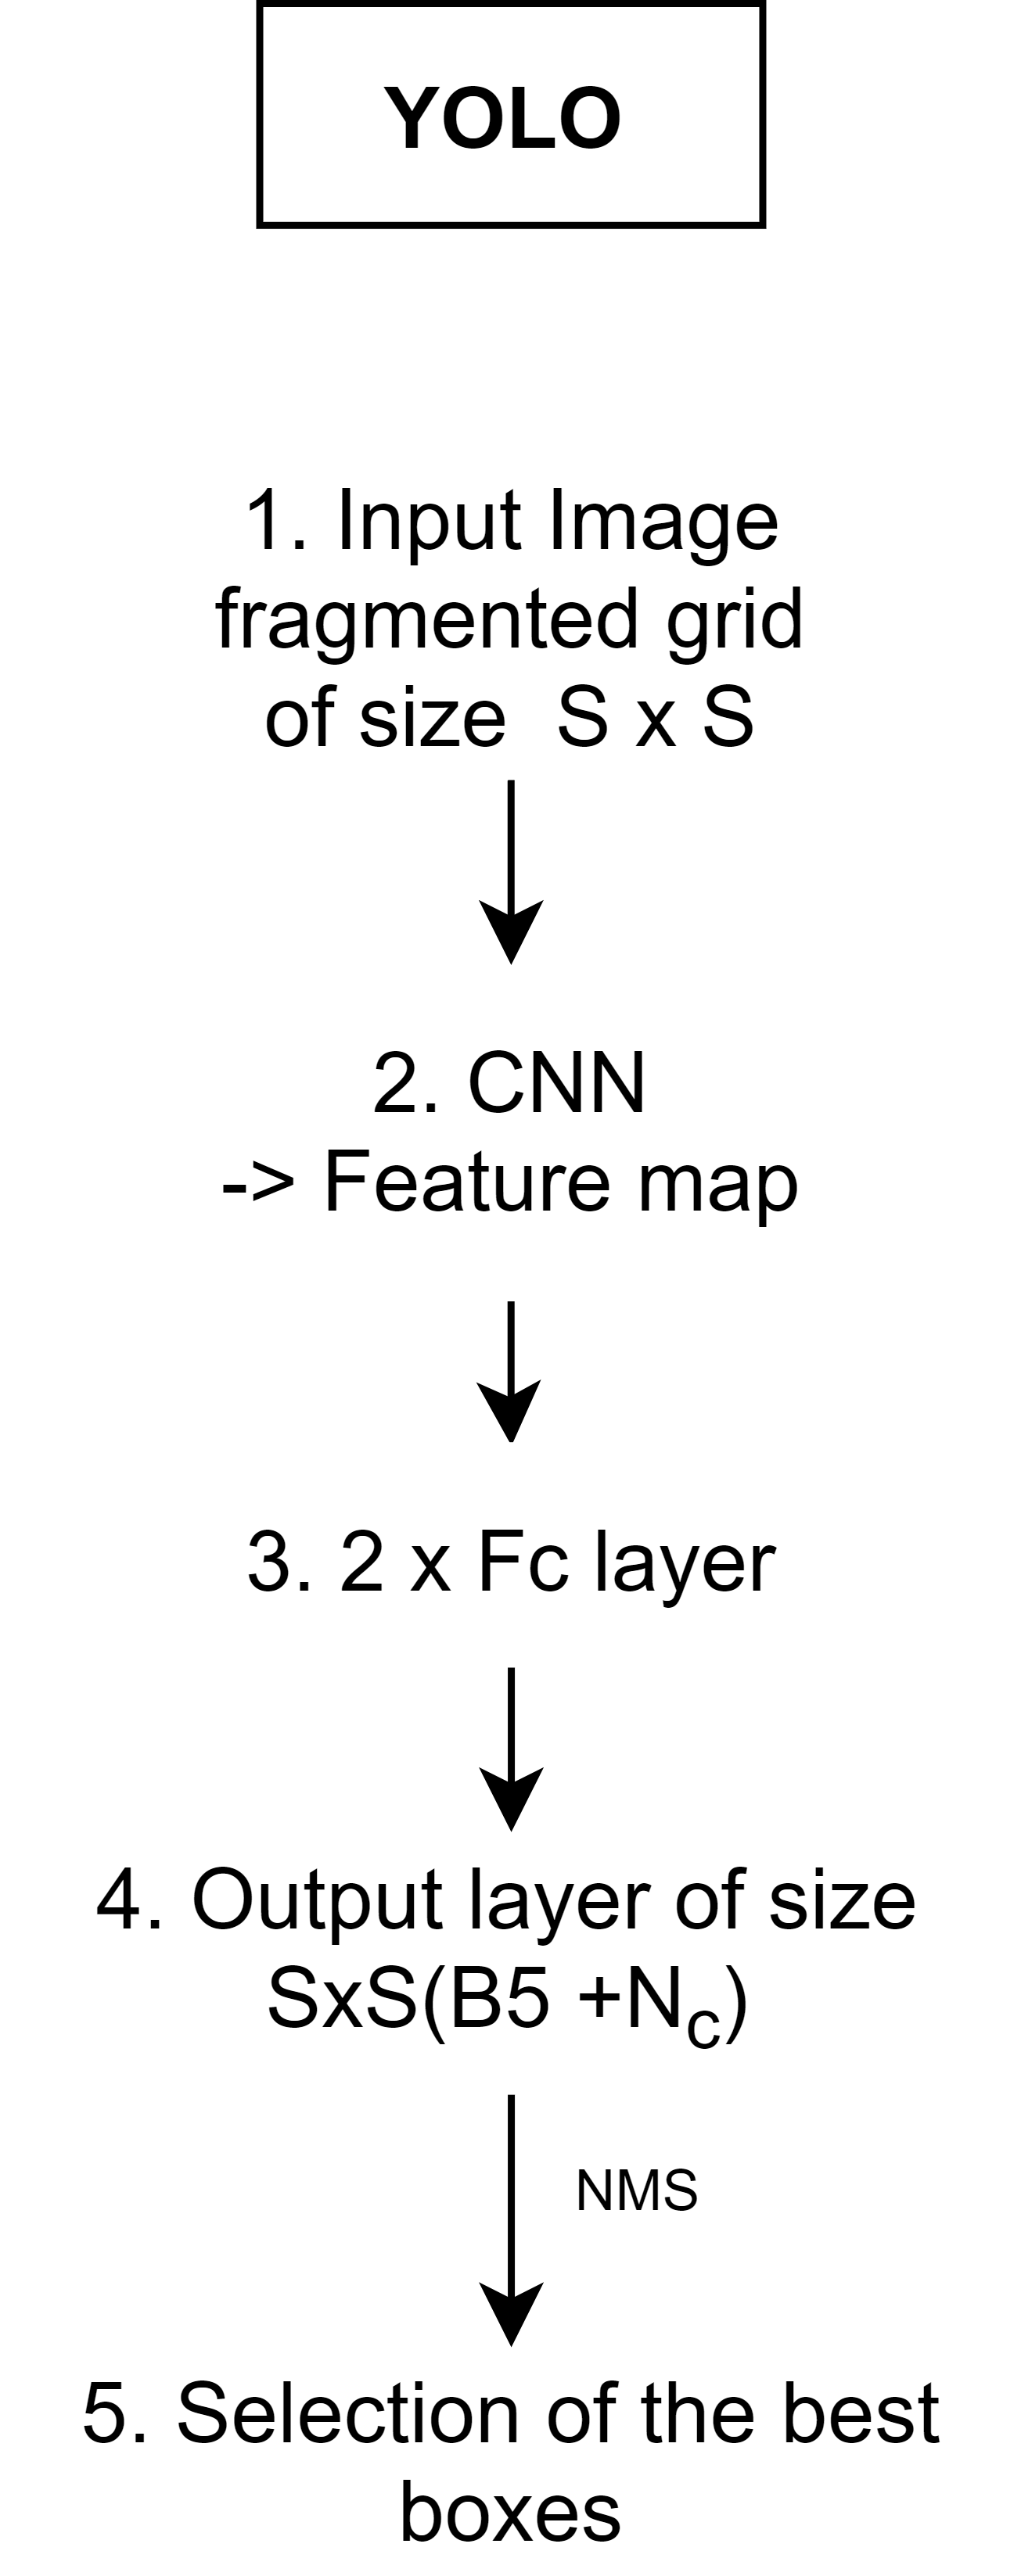
\includegraphics[ height=6cm, keepratio]{figure/Yolo.png}}
% \vspace{-0.6 cm}  % can be changed to suit one's need.
% \caption{Caption}
% \label{}
% \end{figure*}




\begin{figure}[H]
\centering
   \begin{subfigure}{0.3\linewidth}
   \centering
   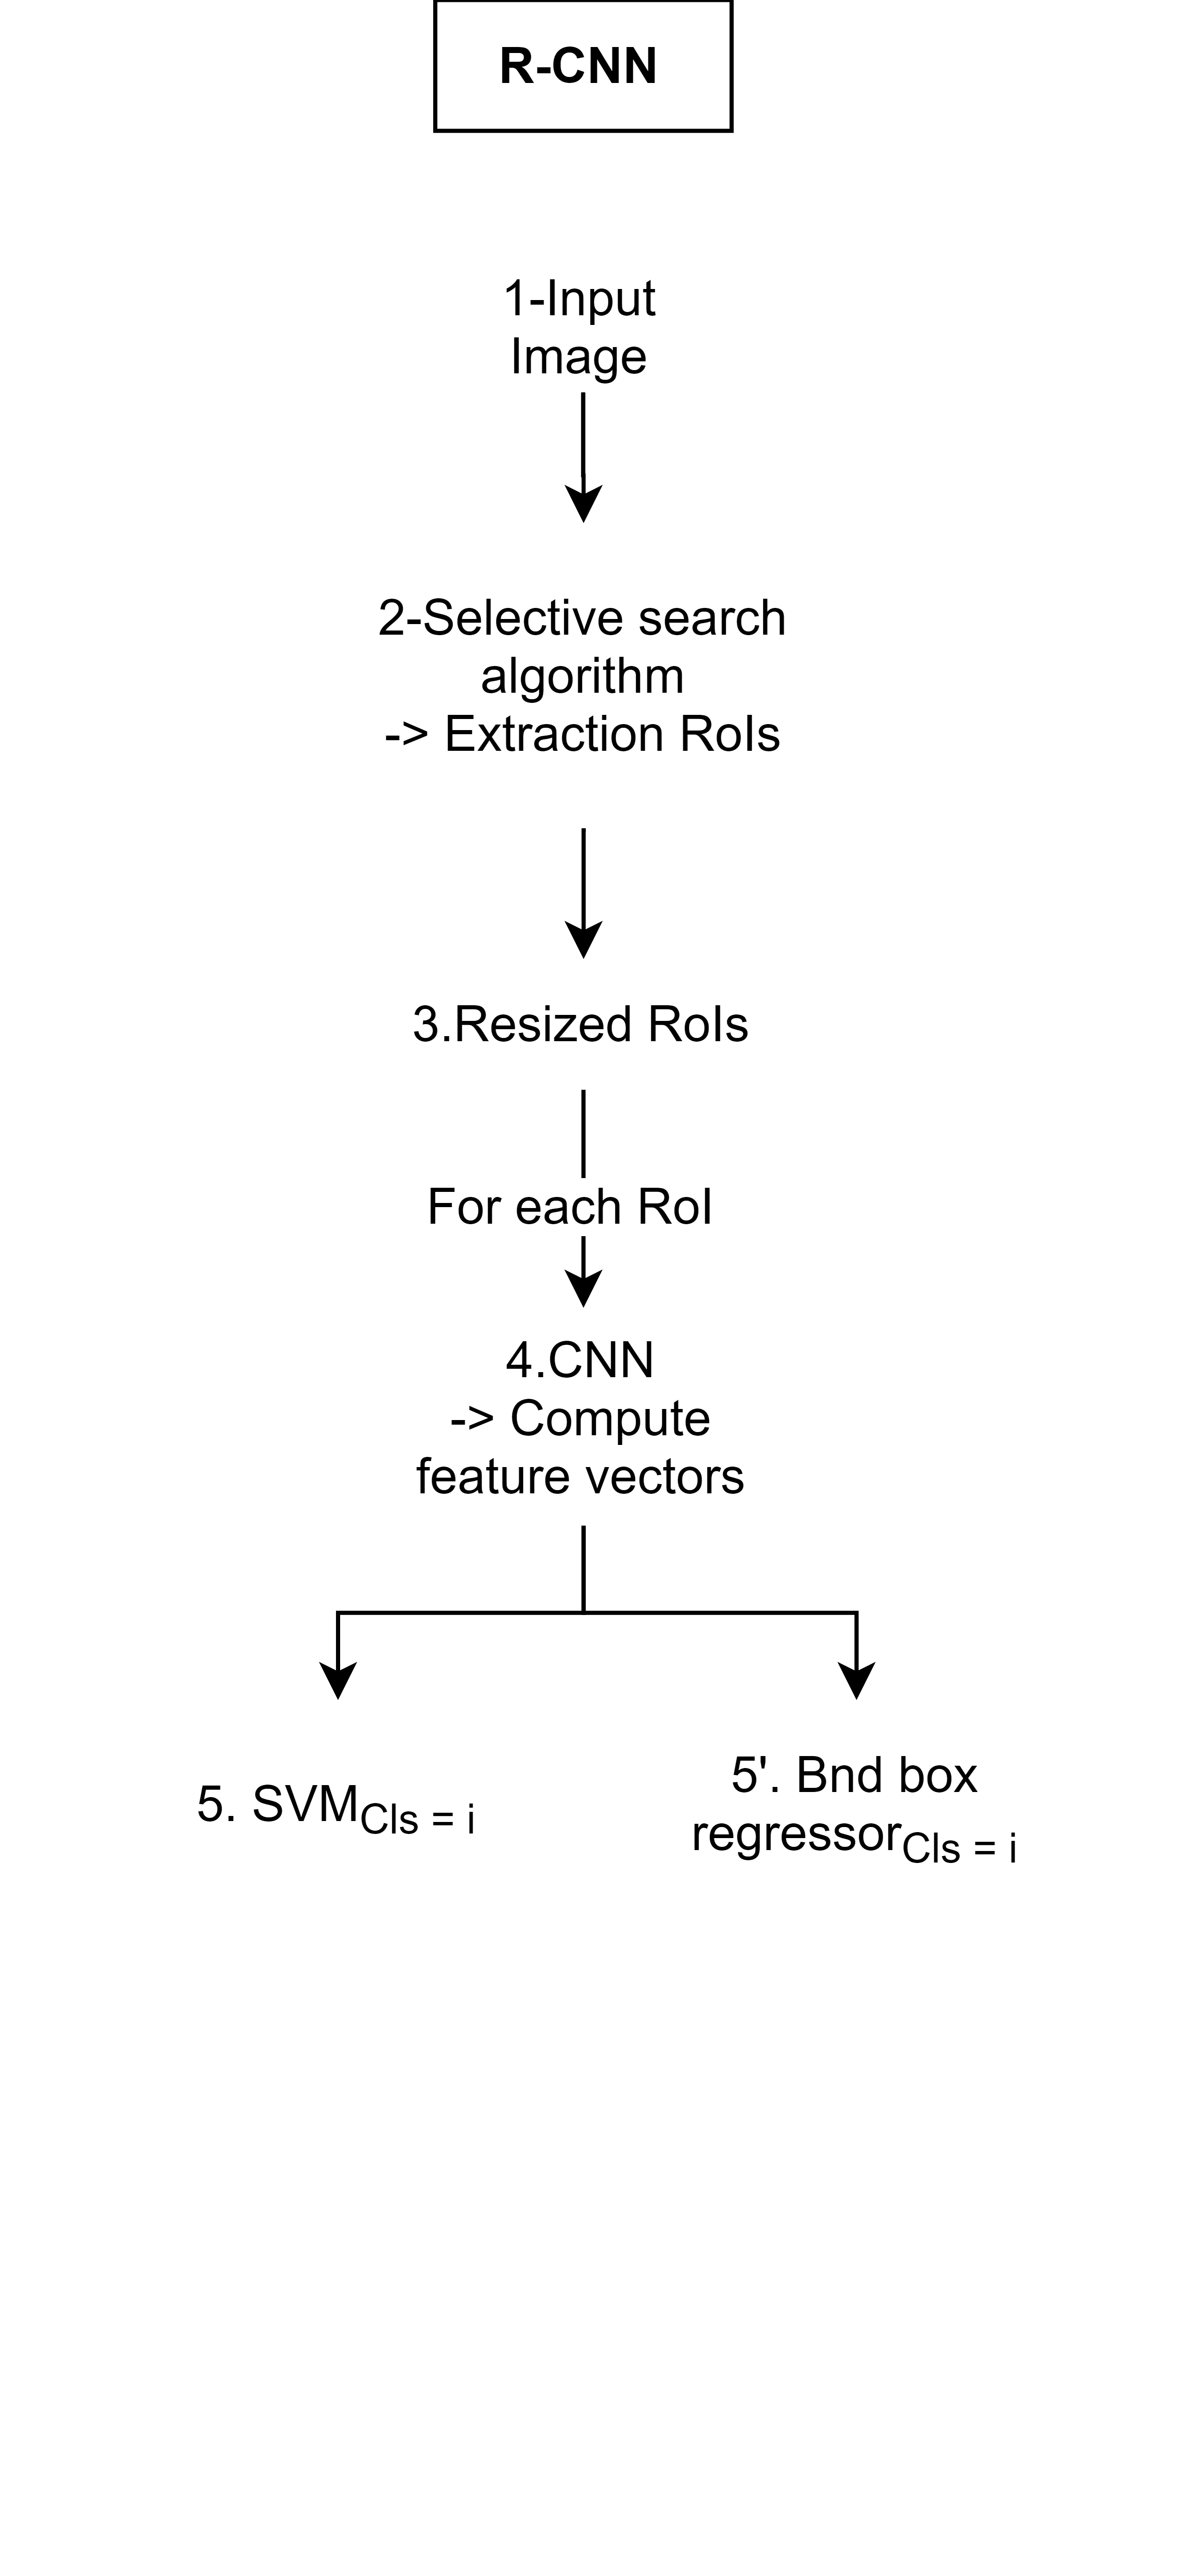
\includegraphics[height=7cm, keepratio]{figure/rcnn_F.png}
   \caption{}
   \label{fig:art_rcnn} 
\end{subfigure}
\hfill
\begin{subfigure}{0.3\linewidth}
   \centering
  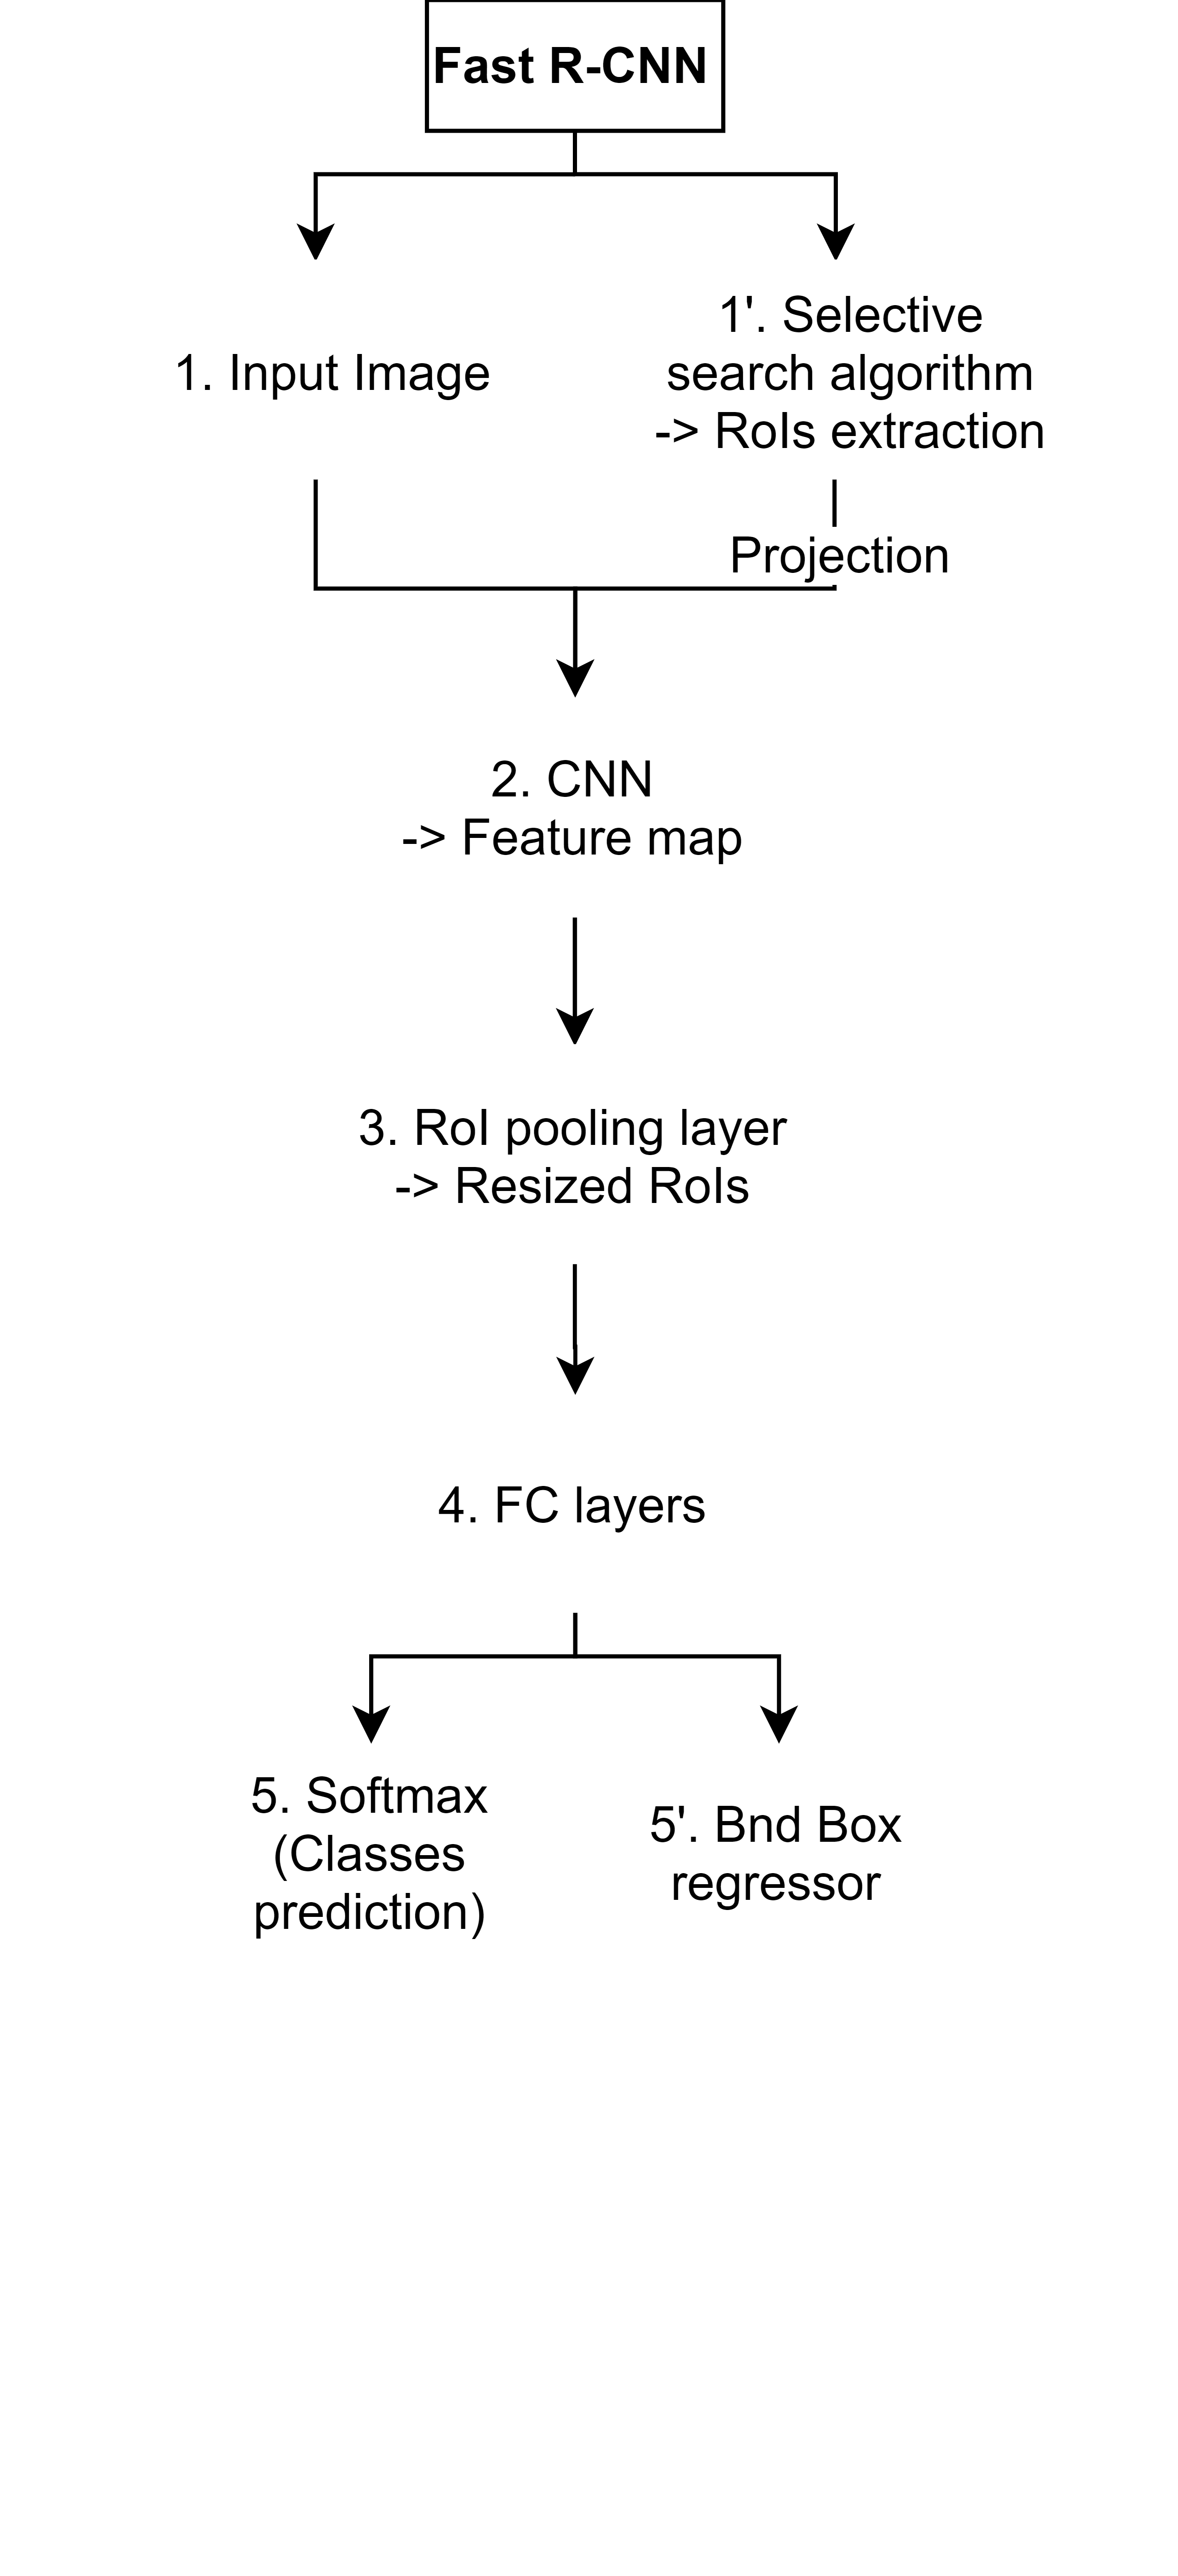
\includegraphics[height=7cm, keepratio]{figure/fast_rcnn_f.png}
   \caption{}
   \label{fig:art_fast_rcnn}
\end{subfigure}
\hfill
\begin{subfigure}{0.3\linewidth}
   \centering
  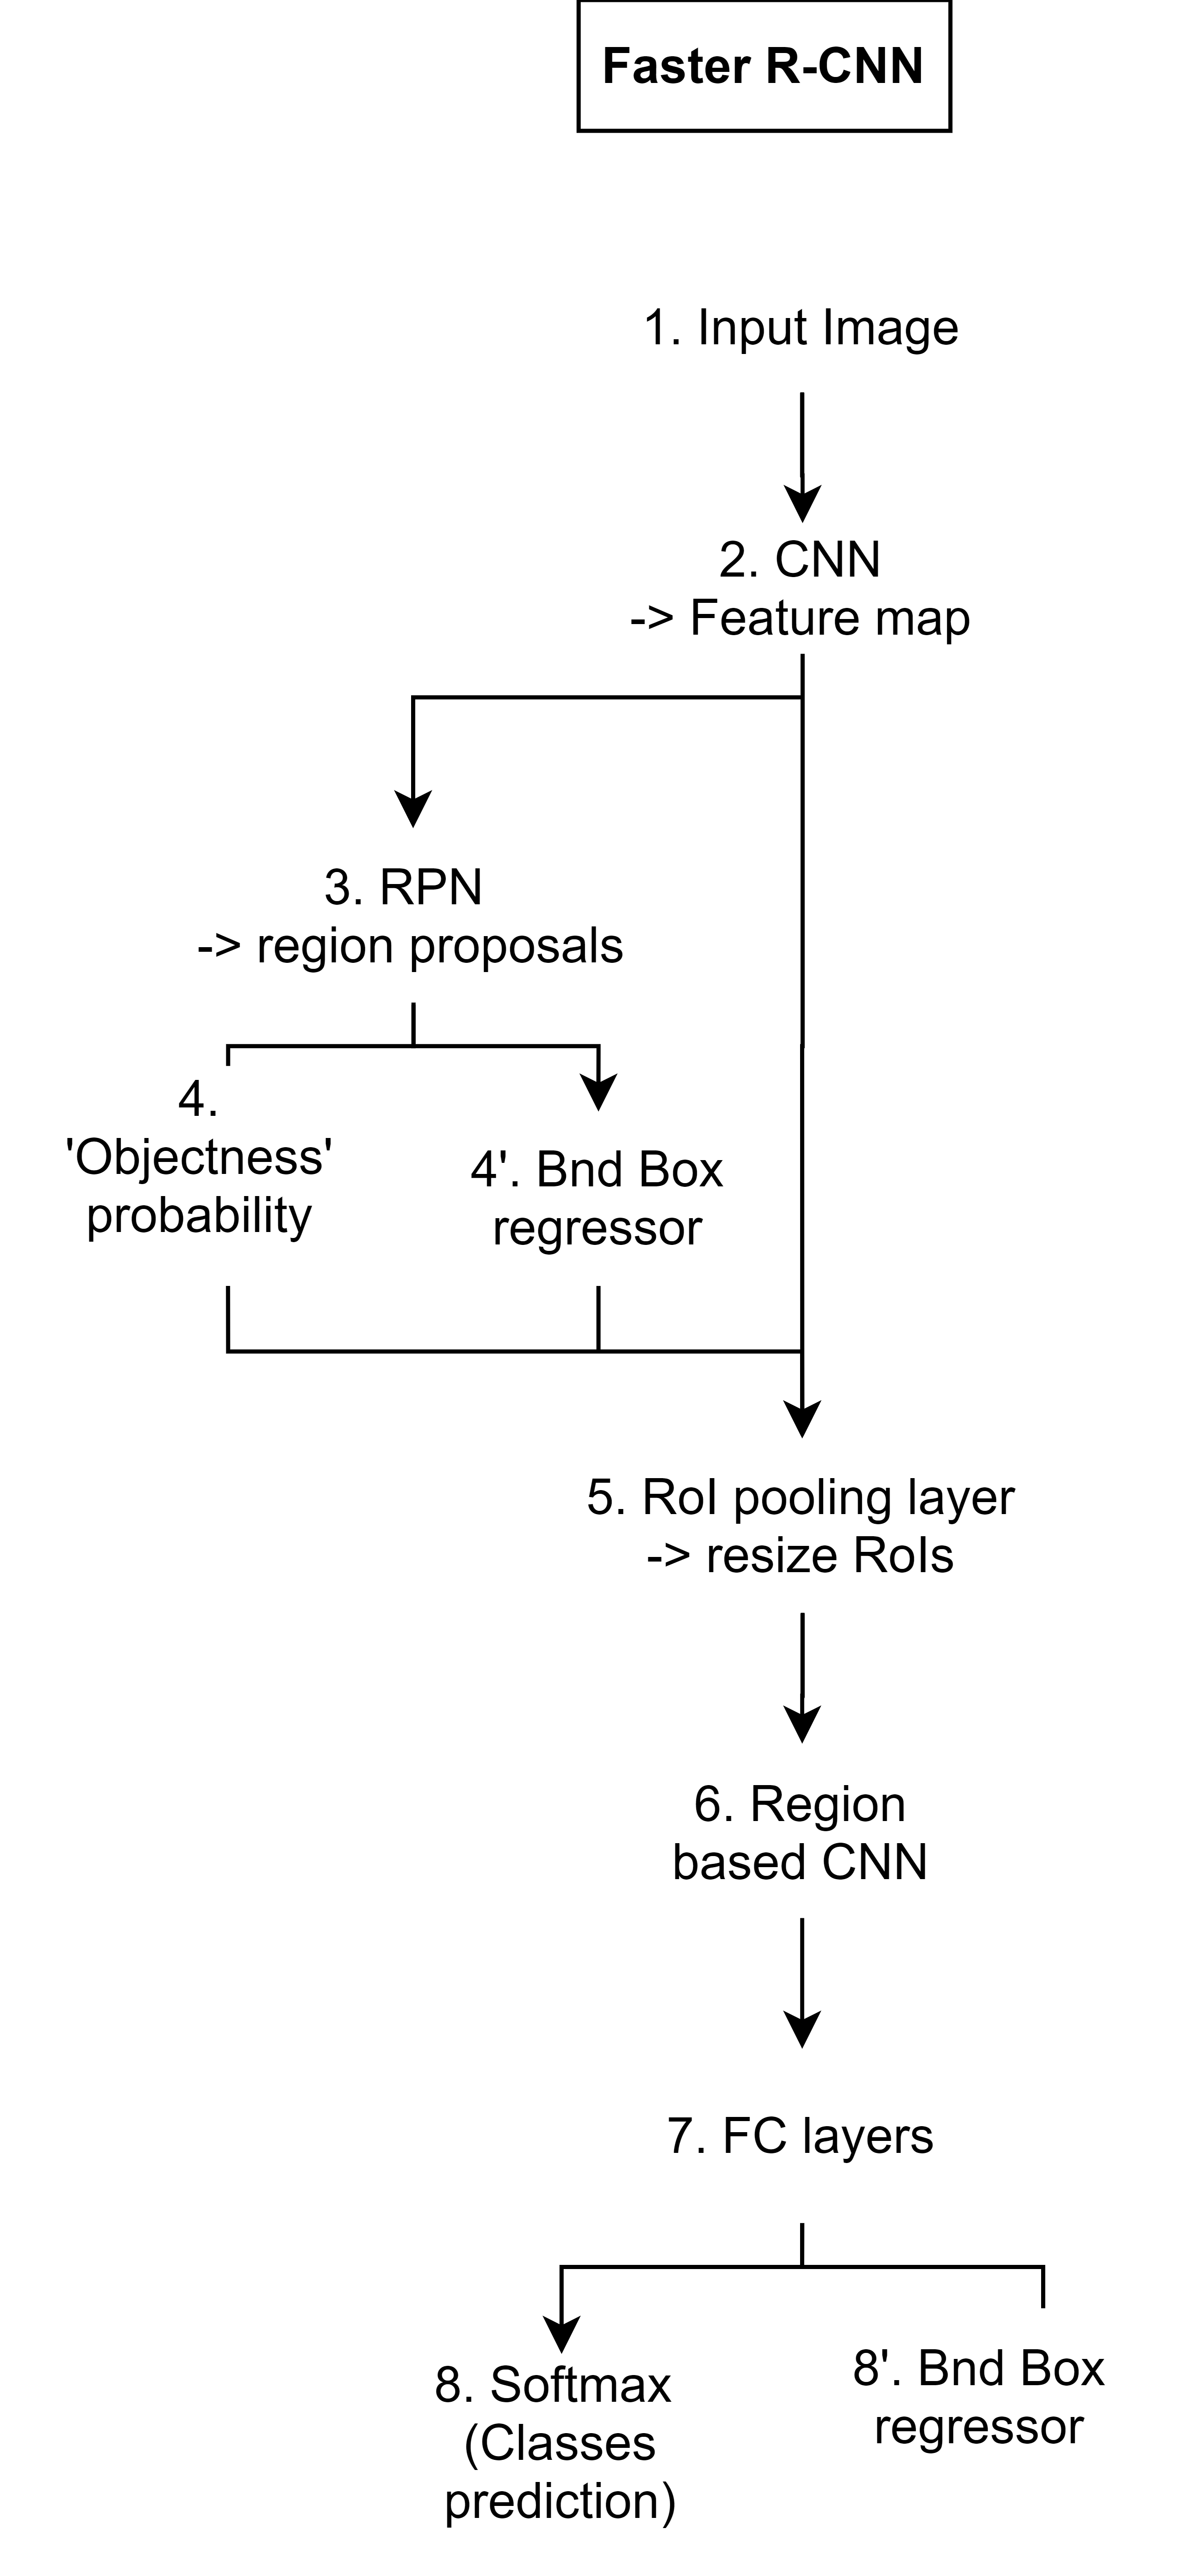
\includegraphics[height=7cm, keepratio]{figure/faster_rcnn_f (1).png}
   \caption{}
   \label{fig:art_faster_rcnn}
\end{subfigure}
\end{figure}%


\begin{figure}[H]\ContinuedFloat
\begin{subfigure}{0.45\linewidth}
   \centering
  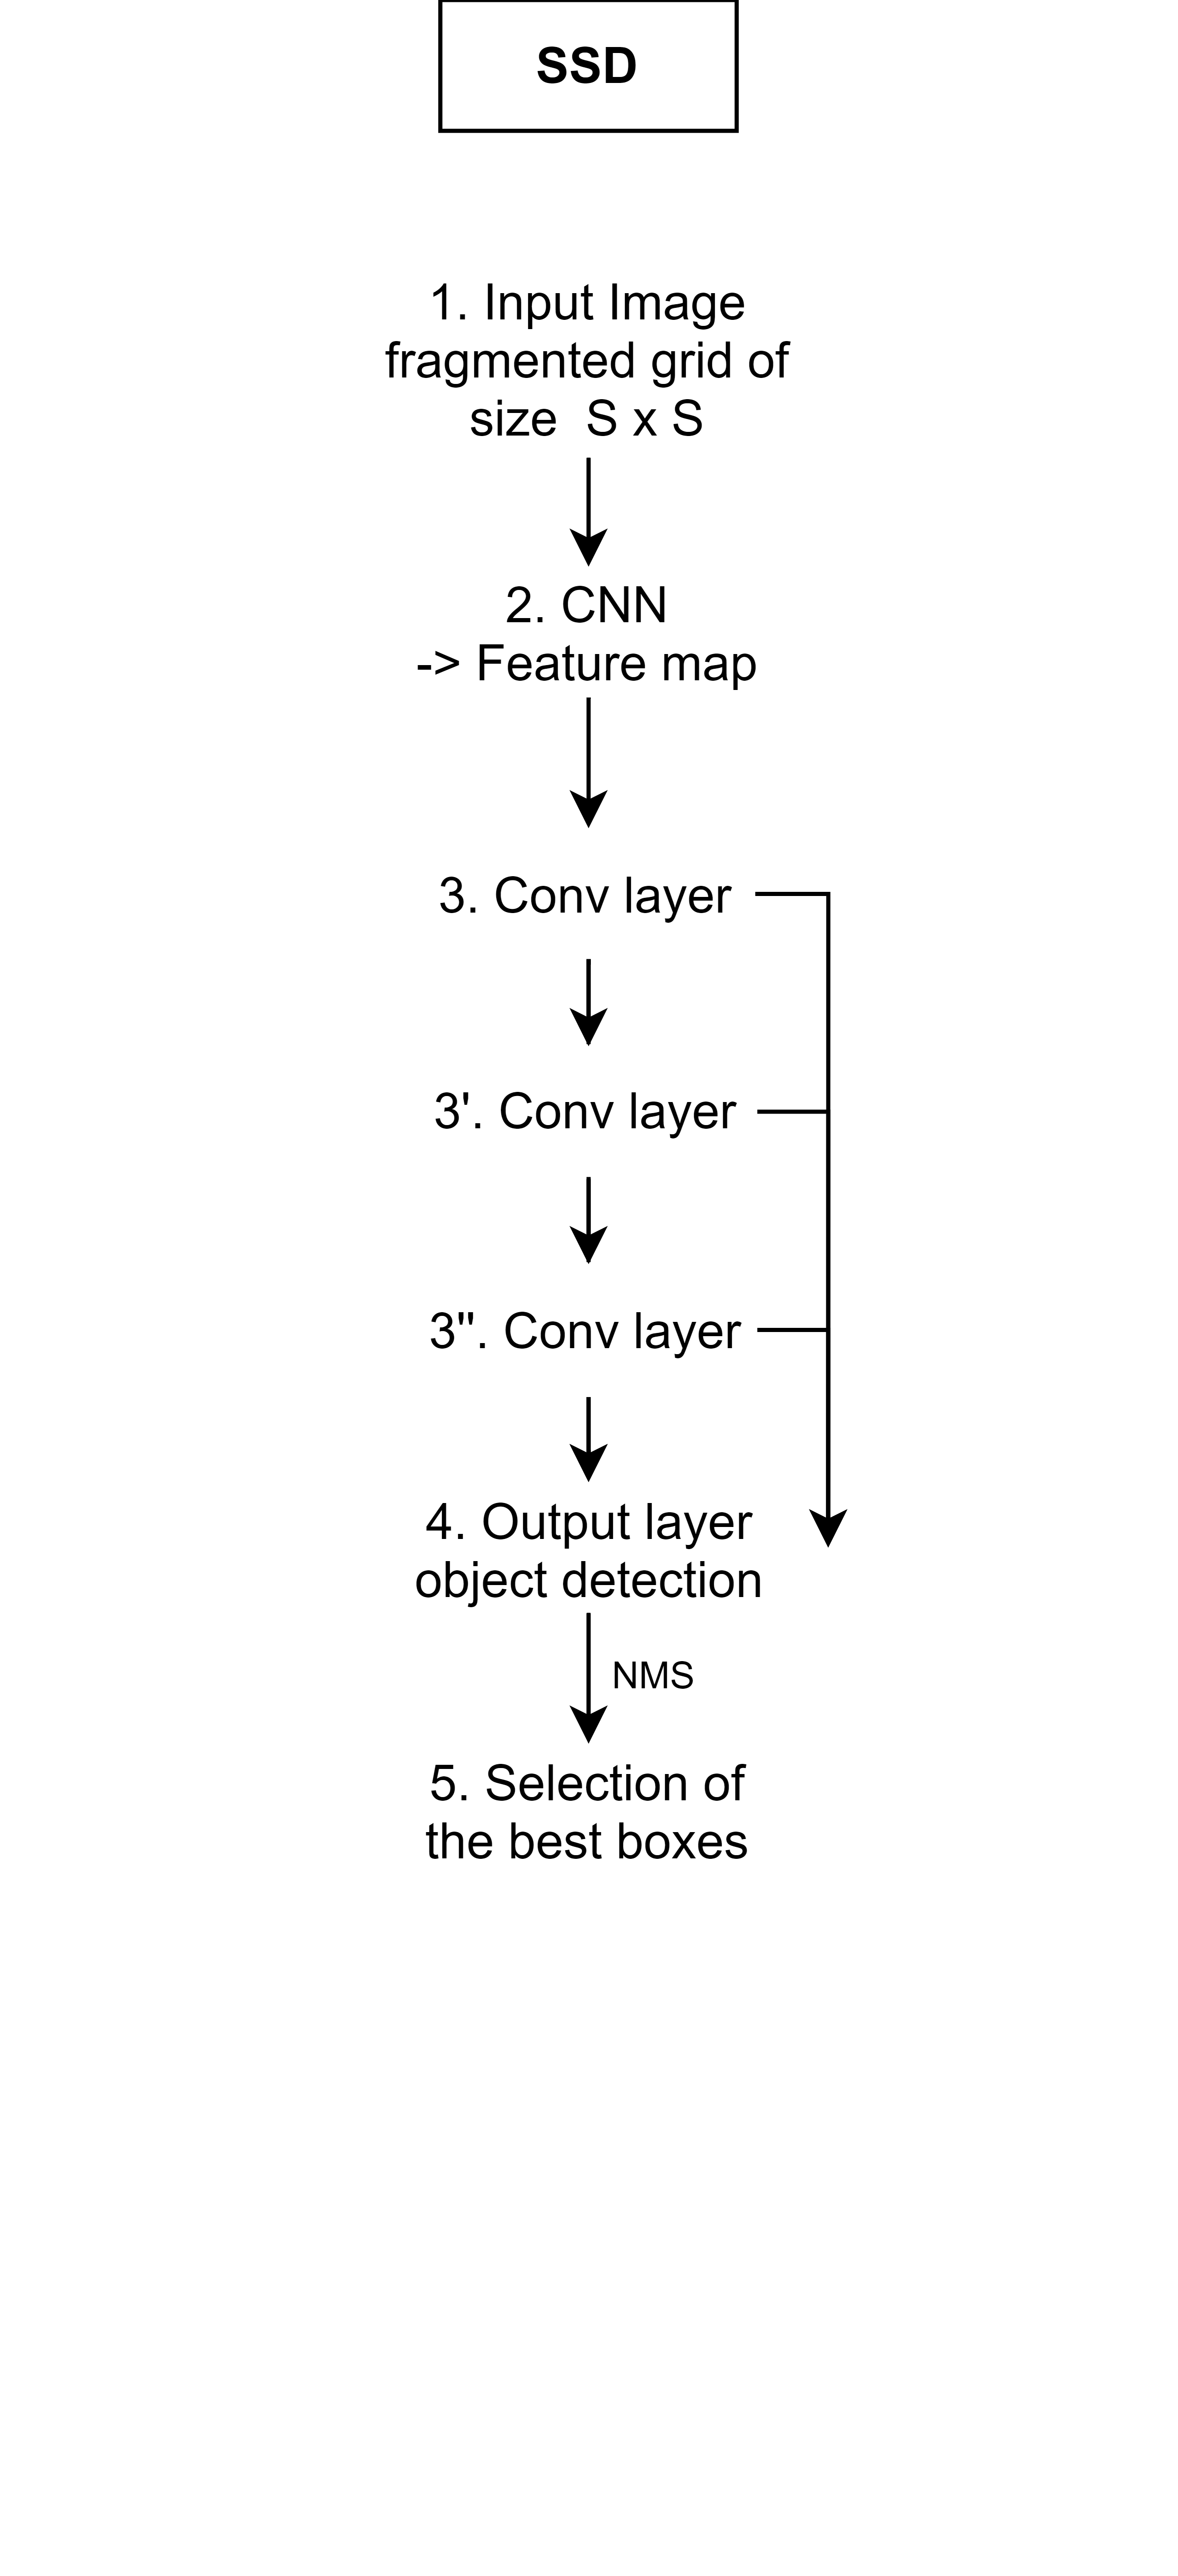
\includegraphics[height=7cm, keepratio]{figure/ssd_f.png}
  \vspace{-1.5cm}
   \caption{}
   \label{art_ssd}
  \end{subfigure}
    ~  \hspace{-2cm}
\begin{subfigure}{0.45\linewidth}
   \centering
  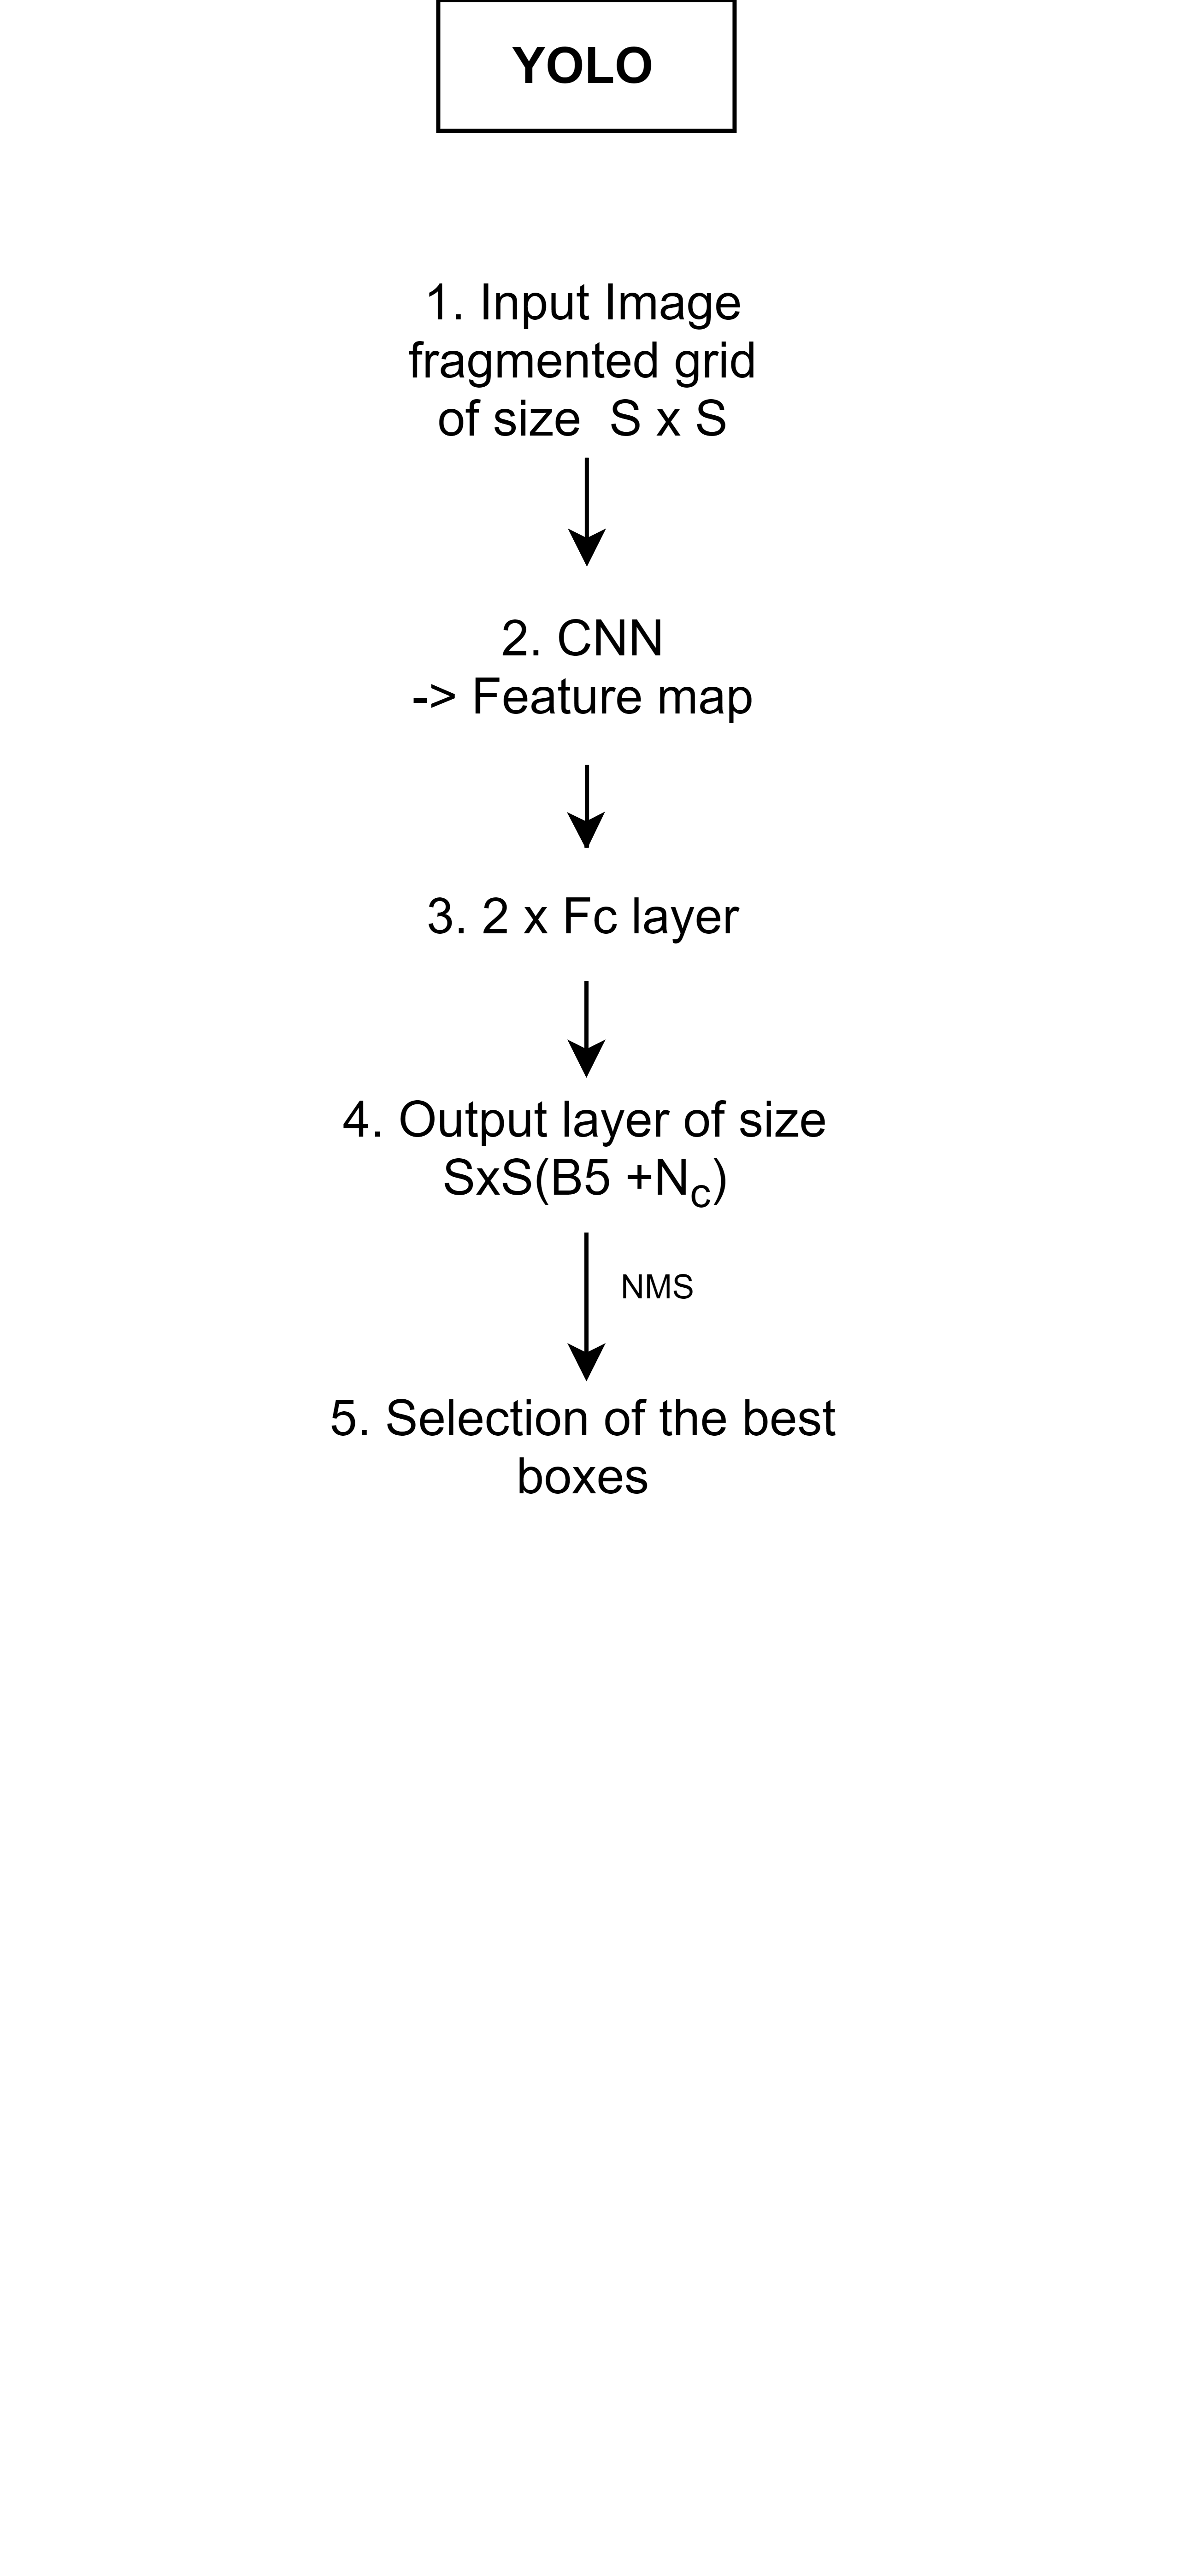
\includegraphics[height=7cm, keepratio]{figure/yolo_f.png}
    \vspace{-1.5cm}
   \caption{}
   \label{fig:art_yolo}
\end{subfigure}
\label{art}
\centering
\caption{(a) Numerical solutions for the constant-curvature body, $F(x)=x(1-x), x \in (0,1)$, at small times. This figure shows the drag force $D$ versus the scaled mass $M$ for various values of the ratio between the inertia $I$ and the mass $M$, i.e. for various values of $R=\frac{I}{M}$. Here $g=10$ and $A=0.7$. (b) As for (a) but with $A=0.5$. (c) As for (a) and (b) but with $A=0.25$.}
\end{figure}







% \begin{figure}[H]
%  \centering
%  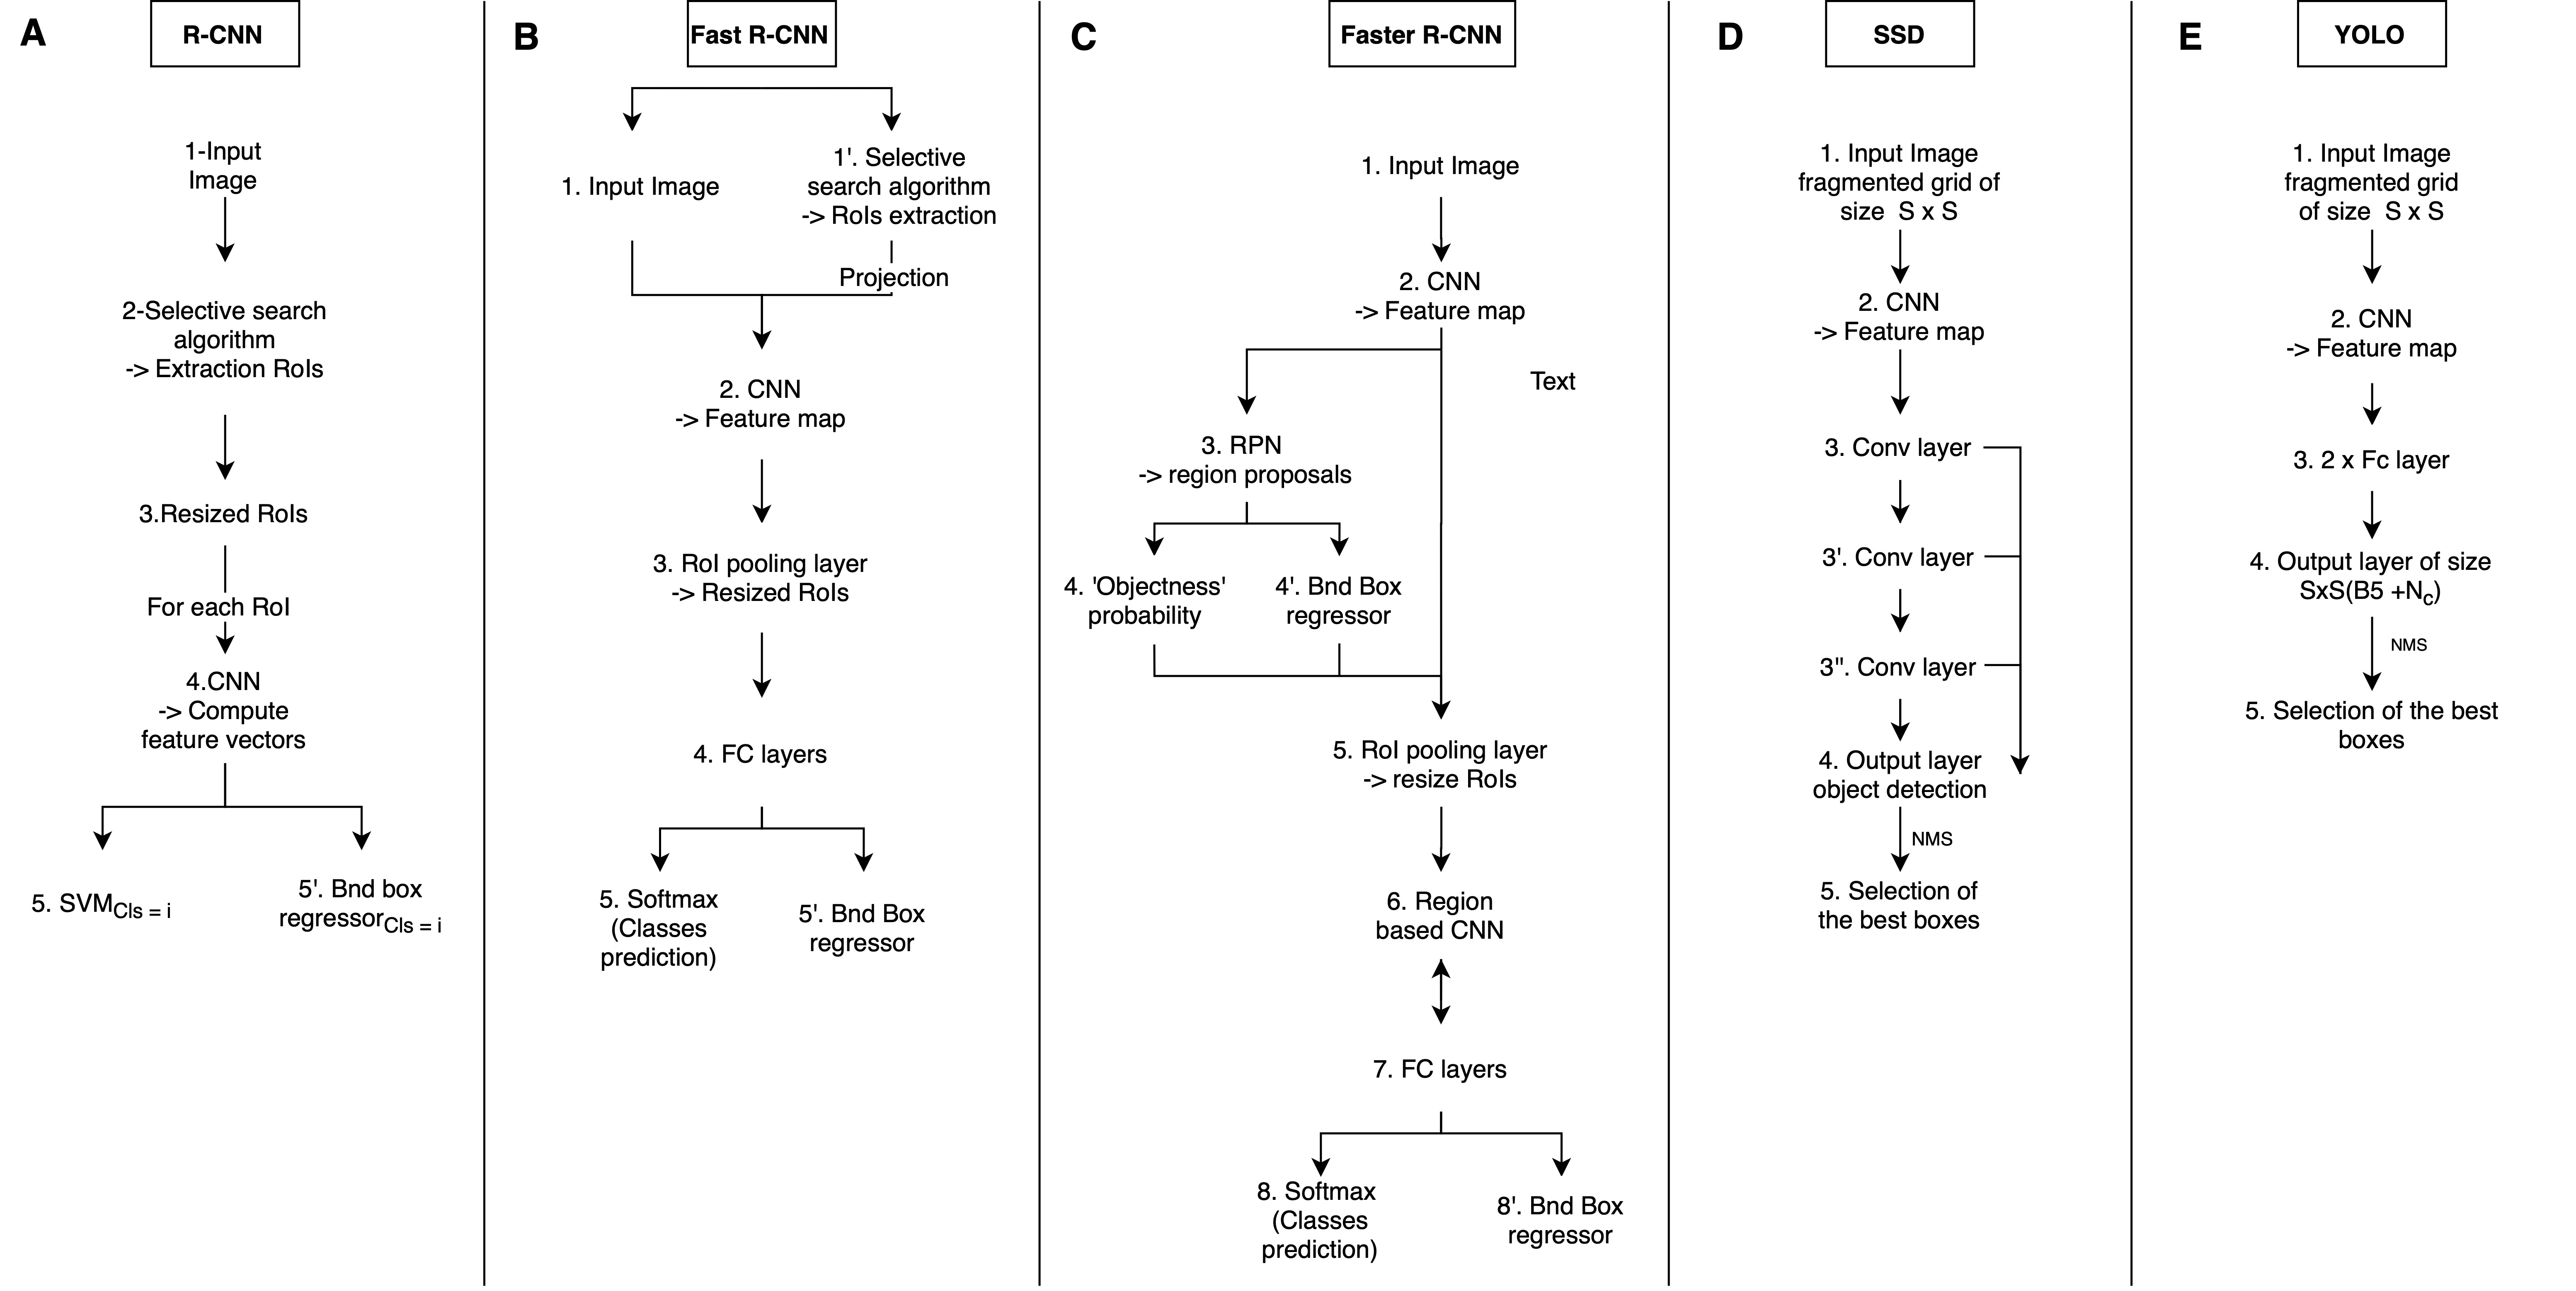
\includegraphics[width=0.9\textwidth]{figure/art-8.jpg}
%  \caption{\textbf{Object detection techniques based on CNNs.} The following diagrams summarizes the main steps of the following object detection techniques: \textbf{A)} \gls{R-CNN} \cite{girshick2015region}, \textbf{B)} Fast \gls{R-CNN} \cite{girshick2015fast}, \textbf{C)} Faster \gls{R-CNN} \cite{ren2015faster}, \textbf{D)} \gls{SSD} \cite{liu2016SSD}, \textbf{E)} \gls{YOLO} \cite{redmon2016you}, where $S$ refers to the grid, $B$ refers to the bounding boxes and $N_c$ to the number of classes (the other abbreviation are list in the index).}
%  \label{Art}
% \end{figure}


\subsection{Description of Faster \gls{R-CNN}}
\subsubsection{Feature network CNN}
Different feature extractors have been implemented for Faster \gls{R-CNN}. The feature extractor\gls{CNN}finally chosen is Inception-v4-ResNet-v2 \cite{szegedy2017inception}, after comparing it with Inception-v2 \cite{szegedy2016rethinking} (\ref{comp_inception_ResNet}). Therefore in the following section, we will describe only described Inception-v4-ResNet-v2.
\\
\underline{\textbf{Inception:}}\\
Inception modules have been developed to answer to information distribution issue, larger kernels should be used for globally distributed information, and reciprocally for local information. Therefore, inception modules use different filter sizes. In addition to not increase the deepness of the network, which are prone to over-fitting and vanishing gradient issue, these filters operate on the same level. Given that convolutional operations are computationally expansive, $1\times1$ filters are applied at modules' entrance, reducing the number of input channels [\textcolor{red}{Fig.}\ref{Ind_ResNet_archi}\textcolor{red}{-B,C,D Turquoise boxes}] \cite{szegedy2015going}. Filter bank expansions are not only computationally cheaper, but they also allow to avoid the representational bottleneck, ie. drastically dimension reduction of the input data [\textcolor{red}{Fig.}\ref{Ind_ResNet_archi}\textcolor{red}{-B, C, D Turquoise boxes}]. Furthermore, to improve the convolutional speed these operations are factorized, for example on the [\textcolor{red}{Fig.}\ref{Ind_ResNet_archi}\textcolor{red}{-C Orange boxes}] the convolutional operation using a filter of size $7\times 7$ is decomposed in two successive operations using filters of size $1\times 7 $ and $7 \times 1$ \cite{szegedy2016rethinking}.Inception-v4 \cite{szegedy2017inception} uses more uniform modules to both boost the performance [\textcolor{red}{Fig.}\ref{Ind_ResNet_archi}\textcolor{red}{-A Green boxes}]. This implementation also used a different upstream network to inception modules [\textcolor{red}{Fig.}\ref{Ind_ResNet_archi}\textcolor{red}{-A Blue box}] and reduction blocks, that modified the width and the height of the grid \cite{szegedy2017inception}.\\
\underline{\textbf{ResNet:}}\\
Many empirical pieces of evidence showed that deeper \gls{CNN}s are able to learn more complex data, justifying the enthusiasm around inception modules. Nevertheless, deeper networks can lead to a degradation of the training accuracy \cite{he2016deep}. Deeper networks are more difficult to optimize and generally suffer from exploding/vanishing gradient problem. ResNet \cite{he2016deep} connections solve this issue by introducing a "deep residual learning framework". Let us consider $H(X)$ as an underlying mapping of a few stack layers with $X$ denoting the input. We define the residual function $F(X)$ such as $F(X)\coloneqq H(X) - X$, like this the original function to optimize become $F(X) + X$ [\textcolor{red}{Fig.}\ref{Ind_ResNet_archi}\textcolor{red}{-E}]. This reformulation solves the degradation problem since if the optimal solution is the identity mapping for a solver it will be easier to set the residual to zero than to learn an identity mapping by multiple non-linear operations. In consequence, a residual network learns the perturbation with the identity mapping as reference. Since $X$ and $F(X)$ must have the same dimension $1\times 1$ convolutional operations are applied after the original operations [\textcolor{red}{Fig.}\ref{Ind_ResNet_archi}\textcolor{red}{-B, C, D, Red elements}]. Furthermore, to respect m the identity mapping should be multiplied by a linear projection $W$, thus the output is: $y : F(X, {W_i}) + W_s X$, where $W_i$ is the matrix of weights.\\
Residual connections integrated with Inception-v4 allows reaching quicker an higher accuracy \ref{comp_inception_ResNet}\textcolor{red}{-B, C}. The purpose of the feature network defined above is to extract an intermediate convolutional layer (\textit{Mixed-6-a}) to build feature map of dimension $D \times D$ [\textcolor{red}{Fig.}\ref{Art}\textcolor{red}{-C Step 2}], that is used to generate region proposals [\textcolor{red}{Fig.}\ref{Art}\textcolor{red}{-C Step 3}].
%-------------------------
\subsubsection{Region Proposals Network (RPN)}
For each point in the feature map, a set of $k$ reference bounding boxes named anchors is defined. These anchors are themself defined by the coordinate of their center $(x,y)$, their width $w$, and their height $h$. To handle objects of different sizes this set of anchors sizes gather boxes of different ratios and sizes. This \gls{RPN} takes as input feature map's windows of size $n\times n$, which are mapped on a lower-dimensional matrix though a convectional layer. Then this matrix fed two parallel convolutional layers. One, with an output of size $2k$, returns for each anchor the probability that it contains an object ("objectness score"). The second one, with an output of size equivalent to $4k$, allows adjusting bounding boxes' coordinates.\\
For the training, each anchor is categorized as a foreground region, if its \gls{IoU}\footnote{\gls{IoU} for Intersection over Union is the ratio of the area shared between two bounding boxes over the area of their union. } with a ground-truth object is higher than 0.7, and as a background region if this ratio is lower than 0.3. The anchors with intermediate \gls{IoU} values are not considered. Then a mini-batch constituted owing to a random sampling of $N$ anchors, with a balanced ratio between the ones classified as foreground and background, is generated, to calculate the multi-task loss function. The function to optimize is defined such as:
\begin{align}
 L({p_i}, {t_i}) = \frac{1}{N_{cls}} \sum_i L_{cls}(p_i, p_i^*) + \lambda \frac{1}{N_{reg}} \sum_i p_i^* L_{reg}(t_i, t_i^*),
 \label{Eq1}
\end{align}
where for the anchor $i$, $p_i$ refers to its "objectness score" and $p_i^*$ is equivalent to 1 if the anchor is classified as a foreground element and to 0 otherwise. The classification loss ($L_{Cls}$) is weighted by $N_{Cls}$ which corresponds to the number of anchors in the mini-batch. The second term of the equation (\ref{Eq1}) represents the regression loss ($L_{reg}$), where $t_i$ is a 4-size vector representing the coordinate of the predicted bounding box, and $t_i^*$ corresponds to the coordinates of the ground-truth bounding box. Given the definition of $p_i^*$ only the anchors classified as foreground elements are taken into account. This second term is weighted by the total number of anchors (ie. $N_{reg} = D\times D \times k$). Finally, the parameter $\lambda$ allows to give weight to the regression part of the optimization function. In more detail, the regression loss is calculated such as: $L_{Reg} = R(t_i - t_i^*)$, where $R$ is the $smooth_L1$ function\footnote{\begin{equation}
 Smooth_{L1}(x) =\begin{cases}
 0.5x^2, & \text{if $|x|<1$}.\\
 |x| - 0.5, & \text{otherwise}.
 \end{cases}
\end{equation} }, allowing to consider as almost correct the bounding boxes with small error. Taking as an example the regression loss calculation on the coordinate $x$, $t_x$ and $t_x^*$ are defined respectively such as: $t_x = (x -x_a) / w_a$ and $t_x^* = (x^* - x_a) / w_a$, where $x$, $x_a$, and $x^*$ correspond respectively to the coordinates of the predicted bounding box, of the anchor and of the ground-truth bounding box. Since the anchors overlap, the proposal regions end up also overlapping the same object, therefore a non-maximal suppression algorithm (\gls{NMS}) \cite{neubeck2006efficient} is used to delete the predicted boxes whose the \gls{IoU} with other predicted boxes is above a given threshold. Finally, the top $N_f$ proposals are kept to be classified. 
\subsubsection{Region-based convolutional network}
Each of the $N_f$ proposals is extracted from the feature map and resized owing to a max-pooling layer [\textcolor{red}{Fig.}\ref{fig:art_faster_rcnn}\textcolor{red}{-step 5}], to get a fixed size matrix. Each of these matrices feeds a Region-based CNN [\textcolor{red}{Fig.}\ref{fig:art_faster_rcnn}\textcolor{red}{-step 6}]. This last network has for objectives to assign a class to each proposal and to adjust their coordinates according to objects' class. To reach this goal, the fixed size matrices are firstly flattened, the resulting vector then feeds 2 \gls{FC} layers [\textcolor{red}{Fig.}\ref{fig:art_faster_rcnn}\textcolor{red}{-step 7}]. The final vector is used to feed two parallel layers. One is used to predict object's class, and so it composed of $\#Classes+1$ units, where $#Classes$ represents the total number of classes in the model more $1$ for the background [\textcolor{red}{Fig.}\ref{fig:art_faster_rcnn}\textcolor{red}{-step 8}]. The second one is used to adjust bounding boxes coordinates, and so it has an output size equivalent to $4\times \# Classes$ [\textcolor{red}{Fig.}\ref{fig:art_faster_rcnn}\textcolor{red}{-step 8'}].


\begin{figure}[H]
 \centering
 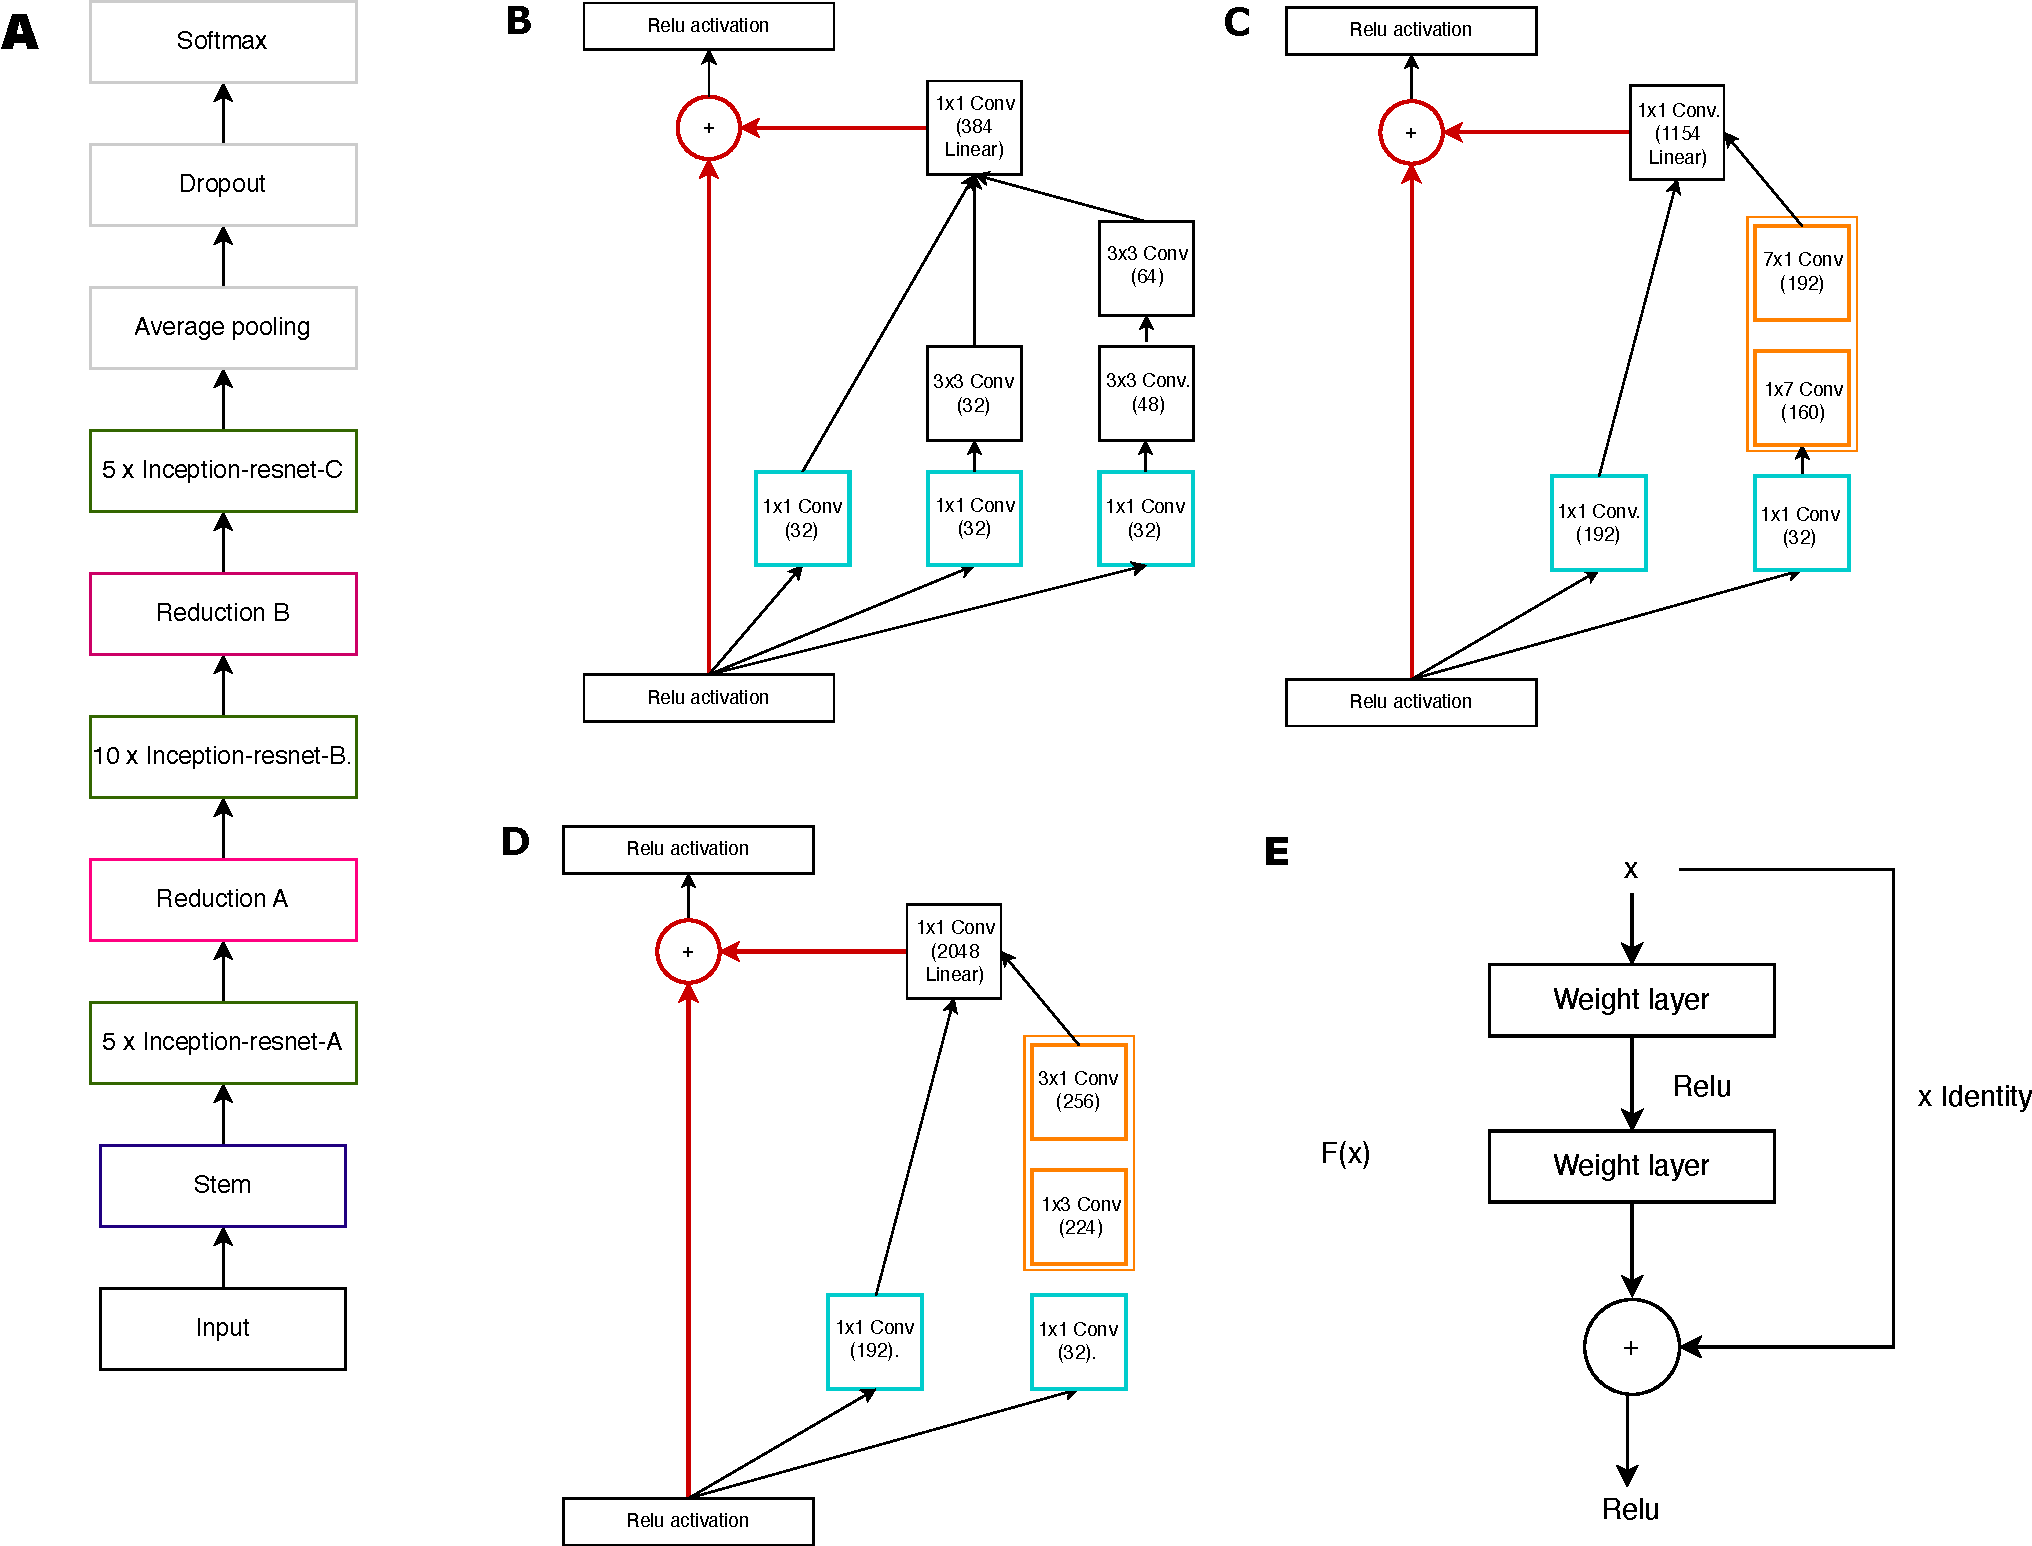
\includegraphics[width=0.9\textwidth]{figure/GLOBAL_NETWORK-2.pdf}

 \caption{\textbf{Architecture's details of the feature extractor network Inception-v4-ResNet-v2.} \textbf{A)} Global architecture of Inception-v4-ResNet-v2. The gray layers are not used in the Faster R-CNN model since an intermediate convolutional layer is extracted to produced the feature map. \textbf{B)} Detail of the block Inception-ResNet A. \textbf{C)} Detail of the block Inception-ResNet B. \textbf{D)} Detail of the block Inception-ResNet C. \textbf{E)} Central dogma of the residual connections.}
 \label{Ind_ResNet_archi}
\end{figure}

\subsection{Training process}
Training a network means to present repetitively pictures for which the outputs are known to calculate the loss function, whose value represents the distance between the predicted and the expected outputs. Therefore, training a network is an optimization problem, consisting of finding the weights that minimize the loss function. This optimization process is done through a gradient descent algorithm \cite{ruder2016overview}. Gradient descent methods allow minimizing a cost function $J(\Theta)$, where $\Theta$ are the model's parameters. Like this, the optimization consists of updating the parameters in the opposite direction of the gradient $\nabla_\Theta J(\Theta)$. The size of the step to reach a minimum is called the learning rate $\eta$. The most basic optimizer is the vanilla gradient descent algorithm, that computes $\nabla_\Theta J(\Theta)$ for the entire data set. Therefore, parameters update is defined by the following equation:
\begin{align}
 \Theta = \Theta - \eta.\nabla_\Theta J(\Theta).
\end{align}

Nevertheless, this algorithm is intractable for large training sets, and suffers from the following drawbacks \cite{ruder2016overview}:
\begin{itemize}
\itemsep0em 
  \item Tuning $\eta$ is a crucial and difficult process. If $eta$ is too small the convergence will be exaggeratedly too slow if it too large $J(\Theta)$ will fluctuate around the minimum;
  \item In deep learning $J(\Theta)$ is often a highly non-convex function, that is why vanilla gradient descent will often get trap in a local minimum. 
\end{itemize}
To overcome these issues, \gls{SGD} is preferred. This method updates the parameters for each training example. For an input matrix $x^{(i)}$ and an output vector $y^{(i)}$, the update equation is:
\begin{align}
 \Theta = \Theta - \eta \nabla_\Theta J(\Theta;x^{(i)}; y^{(i)}).
\end{align}
SGD performs frequent updates that induced high fluctuations in the optimization process. These fluctuations allow escaping local minima but complicate the convergence to the global minimum. Furthermore, SGD has troubles to navigate around very steep minima and oscillate across the slope of ravines \cite{ruder2016overview}. Therefore, the training process has been done with a \gls{SGD} with momentum ($\gamma$). A \gls{SGD} with momentum, adds to each update ($u_t$) a fraction $\gamma$ of the previous update $u_{t-1}$. The parameter update is described by the following equation:
\begin{align}
 u_t &= \gamma u_{t-1} + \eta \nabla_\Theta J (\Theta),\\
 \Theta &= \Theta - u_t.
\end{align}
Then, the update process is described by the following logic:
\begin{align*}
 u_0 &= 0\\
 u_1 &= \gamma u_0 + \eta \nabla_{\Theta_1} J(\Theta_1) = \eta \nabla_{\Theta_1} J(\Theta_1)\\
 u_2& = \gamma u_1 + \eta \nabla_{\Theta_2} J(\Theta_2) = \gamma \eta \nabla_{\Theta_1}J(\Theta_1) + \eta \nabla_{\Theta_2}J(\Theta_2)\\
  u_3& = \gamma u_2 + \eta \nabla_{\Theta_3} J(\Theta_3) = \gamma(\gamma \eta \nabla_{\Theta_1} J(\Theta_1)+\eta \nabla_{\Theta_2} J(\Theta_2)) + \eta \nabla_{\Theta_3} J(\Theta_3)\\
  & ... \\
  u_t &= \gamma u_{t-1} + \eta \nabla_{\Theta_t}) J(\Theta_t) = \gamma^{t-1}\eta \nabla_{\Theta_1}J(\Theta_1)) + \gamma^{t-2}\eta \nabla_{\Theta_2}J(\Theta_2))+ ... + \eta \nabla_{\Theta_t}J(\Theta_t)).
\end{align*}
In analogy with a ball descending a hill, it accumulates momentum and goes faster and faster, with parameters' update momentum term increases when gradients points in the same direction and decreases when gradient change of direction. In consequence, the convergence is faster, and with fewer oscillations \cite{ruder2016overview}. For the training, we set $\gamma = 0.9$.\\
We trained Faster \gls{R-CNN} Inception-v4-Resnet-v2 for 140000 steps ($\simeq 14.4$ epoch). The training time has been defined \textit{a posteriori} according to the convergence of the loss curves of the training and the validation curves. We tuned model's parameters according to Faster \gls{R-CNN} MSCOCO dataset \cite{lin2014microsoft} configuration (\link{https://github.com/tensorflow/models/blob/master/research/\\object_detection/samples/configs/faster_rcnn_inception_resnet_v2_atrous_coco.config}), the main modifications are the following:
\begin{itemize}
\itemsep0em 
 \item Number of classes = 20;
 \item Batch size = 1;
 \item Image resizer: min dimension = 600, max dimension = 600;
 \item Initial learning rate = 0.003;
 \item queue capacity = 2, min after dequeue = 1, num reader = 1\footnote{These parameters allow to handle the quantity of data load at once in the GPU.}.
\end{itemize}
The full configuration file is joined in annex [\ref{config}].
%-----------------------------------------------------------------------------

%_______________________________________________ DATA DESCRIPTION __________________________________________
\subsection{Description of the data set}
Our application works for a set of screws of diameter $3/4$ and $5/8$ inches. For each product, here a product refers to a screw with a particular label, several objects around 5 have been randomly selected. For each object identified by an ID, a video of 5 to 7 seconds has been recorded. To reduce the noise these videos have been realized under a constant powerful artificial light, and width a constant distance between the lens and the object. The screws have been rotated with an angle of $\pm 120$\textdegree, with the 'natural' reading orientation taken as reference ($0$\textdegree). This rotation step fulfills two purposes:
\begin{enumerate}
\itemsep0em 
 \item producing data augmentation,
 \item allowing a learning independent of text orientation, to then give more freedom to users concerning the position of the object under the camera.
\end{enumerate}
These videos have been then segmented to generate around 500 to 600 frames per screw ID. Each frame have to be labeled, \textit{ie.} associating to to an XML file containing the class and the position of each character. For each product, 50 to 100 pictures have been labeled manually with the GUI labelImg (\link{https://github.com/tzutalin/labelImg}). This long and boring process has been shortened owing to a semi-supervised learning protocol. This procedure involves to label manually a small number of pictures around one hundred and to extend the training of the Faster\gls{R-CNN} network using the latest frozen graph by transfer learning. For the labeling purpose, the training set contains all the pictures already labeled from the previous experiments and the ones that just have been manually annotated, and as a test set the remaining pictures to label. Each element in the test set is predicted using the frozen graph of the extended trained model. Predictions' correctness are determined comparing the filenames of the pictures, containing the expected label, and the class of the bounding boxes predicted ordered. This process allowed to re-labeled manually only the picture incorrectly predicted. This protocol could have been used successfully because: 
\begin{itemize}
\itemsep0em 
 \item the pictures data base has been constructed progressively, therefore aside from the first experiment the latest frozen graph could have been used to train a new network by transfer learning;
 \item the same screw IDs are both in the training and in the testing set, this voluntary redundancy ease the labeling process.
\end{itemize} 
After labeling the all data base a fairer training has been launched, where each screw ID belongs either to the training set or to test and/or to the validation set, this allows a more consistent evaluation of model's performances. In the final training, the proportions of pictures in the training, the validation and the test sets are respectively 0.8, 0.05, and 0.15. This split obeys to following rules:
\begin{itemize}
\itemsep0em 
 \item Screws' pictures of the same ID cannot belong to the training set and simultaneously to the validation and/or to the test sets;
\item As far as possible, a balanced ratio of each character is maintained between the three sets;
\item Each product is represented in the training set and in the test or/and in the validation sets. 
\end{itemize}
This second training is needed to guarantee that the model performances are independent from screw IDs.
%-----------------------------------------------------------------------------------------------------------------------------------------------------------
\subsection{Description of the software and hardware environment}
\textbf{\underline{Hardware}}: We worked under Windows 10, with a Lenovo ThinkPad (Intel Core i5 gen 7th). To boost, We have the luck to have a powerful external Processing Unit \gls{GPU} with the following characteristics:

 
\begin{table}[h]
\begin{center}
\begin{tabular}{|l|l|}
\hline
\textbf{Model}  & Razor GEFORCE RTX 2080 TI GAMING X TRIO \\ \hline
\textbf{GPU}   & Nvidia GetForce RTX 2080Ti    \\ \hline
\textbf{Architecture} & Nvidia Turing       \\ \hline
\textbf{Boost Clock} & 1545 MHz         \\ \hline
\textbf{Cuda Core} & 4352          \\ \hline
\textbf{Memory size} & 11 GB         \\ \hline
\textbf{Memory bus} & 352 Bit         \\ \hline
\end{tabular}
\caption{external GPU features}
\end{center}
\end{table}
 Videos have been recorded with a Basler ace acA1920-150um Monochrome USB 3.0 camera, installed on a metal support guarantying a constant distant between the lens and the object, this support is also equipped with a light. 
%________________________________
\hspace{-0.8cm}\textbf{\underline{Software}}: We used the official Tensorflow object API (\link{https://github.com/tensorflow/models/tree/ \\ master/research/object\_detection}) to create our training platform. We re-used the models' architecture \cite{szegedy2017inception, huang2017speed, ren2015faster}, and supported files such as box\_coder, anchors\_generator, metrics... We used Tensorboard API (\link{https://github.com/tensorflow/tensorboard}) to follow training and validation's progress. We worked under a Python (3.7) virtual envirnoment whose the main libraries are Tensorflow-gpu = 1.15 and OpenCV = 4.2. To use the \gls{GPU}, we installed CUDA Toolkit 10.0 (\link{https://developer.nvidia.com/cuda-10.0-download-archive}) and Cudnn 7.6.4 (\link{https://developer.nvidia.com/rdp/cudnn-archive}). Finally, the \gls{GUI} has been using PyQT5 (\link{https://wiki.python.org/moin/PyQt}).
%_______________________________________________________________________________
\subsection{Training process}
Training a network means to present repetitively pictures for which the outputs are known to calculate the loss function, whose value represents the distance between the predicted and the expected outputs. Therefore, training a network is an optimization problem, consisting of finding the weights that minimize the loss function. This optimization process is done through a gradient descent algorithm \cite{ruder2016overview}. Gradient descent methods allow minimizing a cost function $J(\Theta)$, where $\Theta$ are the model's parameters. Like this, the optimization consists of updating the parameters in the opposite direction of the gradient $\nabla_\Theta J(\Theta)$. The size of the step to reach a minimum is called the learning rate $\eta$. The most basic optimizer is the vanilla gradient descent algorithm, that computes $\nabla_\Theta J(\Theta)$ for the entire data set. Therefore, parameters update is defined by the following equation:
\begin{align}
 \Theta = \Theta - \eta.\nabla_\Theta J(\Theta).
\end{align}

Nevertheless, this algorithm is intractable for large training sets, and suffers from the following drawbacks \cite{ruder2016overview}:
\begin{itemize}
\itemsep0em 
  \item Tuning $\eta$ is a crucial and difficult process. If $eta$ is too small the convergence will be exaggeratedly too slow if it too large $J(\Theta)$ will fluctuate around the minimum;
  \item In deep learning $J(\Theta)$ is often a highly non-convex function, that is why vanilla gradient descent will often get trap in a local minimum. 
\end{itemize}
To overcome these issues, \gls{SGD} is preferred. This method updates the parameters for each training example. For an input matrix $x^{(i)}$ and an output vector $y^{(i)}$, the update equation is:
\begin{align}
 \Theta = \Theta - \eta \nabla_\Theta J(\Theta;x^{(i)}; y^{(i)}).
\end{align}
SGD performs frequent updates that induced high fluctuations in the optimization process. These fluctuations allow escaping local minima but complicate the convergence to the global minimum. Furthermore, SGD has troubles to navigate around very steep minima and oscillate across the slope of ravines \cite{ruder2016overview}. Therefore, the training process has been done with a \gls{SGD} with momentum ($\gamma$). A \gls{SGD} with momentum, adds to each update ($u_t$) a fraction $\gamma$ of the previous update $u_{t-1}$. The parameter update is described by the following equation:
\begin{align}
 u_t &= \gamma u_{t-1} + \eta \nabla_\Theta J (\Theta),\\
 \Theta &= \Theta - u_t.
\end{align}
Then, the update process is described by the following logic:
\begin{align*}
 u_0 &= 0\\
 u_1 &= \gamma u_0 + \eta \nabla_{\Theta_1} J(\Theta_1) = \eta \nabla_{\Theta_1} J(\Theta_1)\\
 u_2& = \gamma u_1 + \eta \nabla_{\Theta_2} J(\Theta_2) = \gamma \eta \nabla_{\Theta_1}J(\Theta_1) + \eta \nabla_{\Theta_2}J(\Theta_2)\\
  u_3& = \gamma u_2 + \eta \nabla_{\Theta_3} J(\Theta_3) = \gamma(\gamma \eta \nabla_{\Theta_1} J(\Theta_1)+\eta \nabla_{\Theta_2} J(\Theta_2)) + \eta \nabla_{\Theta_3} J(\Theta_3)\\
  & ... \\
  u_t &= \gamma u_{t-1} + \eta \nabla_{\Theta_t}) J(\Theta_t) = \gamma^{t-1}\eta \nabla_{\Theta_1}J(\Theta_1)) + \gamma^{t-2}\eta \nabla_{\Theta_2}J(\Theta_2))+ ... + \eta \nabla_{\Theta_t}J(\Theta_t)).
\end{align*}
In analogy with a ball descending a hill, it accumulates momentum and goes faster and faster, with parameters' update momentum term increases when gradients points in the same direction and decreases when gradient change of direction. In consequence, the convergence is faster, and with fewer oscillations \cite{ruder2016overview}. For the training, we set $\gamma = 0.9$.\\
We trained Faster \gls{R-CNN} Inception-v4-Resnet-v2 for 140000 steps ($\simeq 14.4$ epoch). The training time has been defined \textit{a posteriori} according to the convergence of the loss curves of the training and the validation curves. We tuned model's parameters according to Faster \gls{R-CNN} MSCOCO dataset \cite{lin2014microsoft} configuration (\link{https://github.com/tensorflow/models/blob/master/research/\\object_detection/samples/configs/faster_rcnn_inception_resnet_v2_atrous_coco.config}), the main modifications are the following:
\begin{itemize}
\itemsep0em 
 \item Number of classes = 20;
 \item Batch size = 1;
 \item Image resizer: min dimension = 600, max dimension = 600;
 \item Initial learning rate = 0.003;
 \item queue capacity = 2, min after dequeue = 1, num reader = 1\footnote{These parameters allow to handle the quantity of data load at once in the GPU.}.
\end{itemize}
The full configuration file is joined in annex [\ref{config}].
%-----------------------------------------------------------------------------
 \subsection{Metrics to evaluate model's performances}
 During the training, to evaluate model's performances we follow the metrics show by Tensorboard, \textit{ie.} the loss curves [\textcolor{red}{Fig.}\ref{comp_inception_ResNet}\textcolor{red}{-A}], the \gls{mAP} [\textcolor{red}{Fig.}\ref{comp_inception_ResNet}\textcolor{red}{-B}] and the \gls{AR} [\textcolor{red}{Fig.}\ref{comp_inception_ResNet}\textcolor{red}{-C}]. At the end of the training, we predicted the full data set, generating XML files containing for each bounding box predicted its location, its class, and its accuracy. Then we compared the expected XML files with the predicted ones according to the following protocole:
 \begin{enumerate}
 \itemsep0em 
  \item For each bounding box $i$ predicted we search in the expected XML file the bounding box $j$ with the maximal \gls{IoU}.
  \item If $IoU_{i,j}> 0.7$, $i$ is classified as a \gls{TP}, and as a \gls{FP} otherwise.
  \item Furthermore, if $class_i = class_j$, $i$ is labeled as well-classified and as miss-classified otherwise.
  \item Each expected bounding box not found in the expected XML file are classified as \gls{FN}.
 \end{enumerate}
This process applied successfully to the train, the validation and the test sets allow generating the following metrics:
\begin{itemize}
\itemsep0em 
 \item Global metrics:
   \begin{itemize}
   \itemsep0em 
    \item Proportion of images fully correctly predicted;
    \item Total proportion of character correctly predicted;
    \item Proportion of images per screw label correctly predicted, to catch if one label has ot been learned [\textcolor{red}{Fig.}\ref{comp_inception_ResNet}\textcolor{red}{-D,F}];
    \item Proportion of images per screw ID correctly predicted, as an indicator of potential poor quality picture associated to an object.
   \end{itemize}
 \item Bounding boxes metrics: 
 \begin{itemize}
 \itemsep0em 
  \item Total proportion of \gls{TP}, \gls{FP}, \gls{FN}.
 \end{itemize}
  \item Character metrics:
  \begin{itemize}
  \itemsep0em 
   \item Recall per character, to asses model's sensitivity;
   \item Precision per character;
   \item Errors occurrences [\textcolor{red}{Fig.}\ref{comp_inception_ResNet}\textcolor{red}{-E,G}];
   \item Accuracy distribution per character.
  \end{itemize}
\end{itemize}
Accuracy distributions were used to assess character readability, we noticed that despite of very narrow distribution center on 0.99, that this metrics can be used to generate warnings if character's accuracy is too low. 

%___________________________________________________________________________________________________

\subsection{Blind comparison between the expected and the predicted label}
When a new picture is predicted the question around comparing the expected and predicted text appears trivial but it is not because of the different possible screws orientations. Once the prediction is made, two cluster are created owing to a K-Means algorithm to separate the cluster of letters and the cluster of numbers, bounding boxes associated with the Hilti's logo forms an another cluster [\textcolor{red}{Fig.}\ref{blind}\textcolor{red}{-column 1}]. The main orientation of the two clusters are then determined. If the cluster is horizontally orientated [\textcolor{red}{Fig.}\ref{blind}\textcolor{red}{-case 1}], the bounding box associated to the minimal $x$ coordinate constitutes the extremity of a linking chain, reciprocally if the cluster vertically orientated [\textcolor{red}{Fig.}\ref{blind}\textcolor{red}{-case 2,3}] the bounding box associated with the minimal $y$ coordinate defines the extremity. From this extremity, the linking chain mentioned, associates to the last element included its first closest neighbor not already included in the linking chain. For the two clusters, this process allows generating two list of bounding boxes ordered by bounding boxes coordinates. Then the two resulting of list are order in order to position the elements corresponding to the cluster of letters in front. Finally the famous algorithm of Needleman and Wunsch algorithm \cite{spr1970general} is used to align the expected label and the predicted one, after bounding box sorting. According to the screw orientation the linking chain build have to be reversed [\textcolor{red}{Fig.}\ref{blind}\textcolor{red}{-case 3}]. Therefore, two alignments are calculated and the one associated to the best score is kept. The algorithm of Needleman and Wunsch is also used to align the logo, if the reverse solution is retained the logo text is also reversed. The described strategy answer to most of the cases but it is not exhaustive, for examples: 
\begin{itemize}
\itemsep0em 
 \item if a full cluster is predicted in reversed order the reversion operation will canceled this misclassification, \textit{eg.} for a expected cluster "KH" if the prediction is "HK" the reversion operation implies that the prediction becomes "KH";
 \item if a miss-classification is upstream of \gls{FN}, \gls{FN} position are difficult to determines. 
\end{itemize} 
Given the extremely good performances of the model, despite of these rare exceptions this strategy has been retained.
%___________________________________________________________________________________________________

\subsection{Detection of damaged characters}
Object detection algorithms allow the classification and the localization of objects. This property answers to the first problematic that it is to say allow guaranteeing that the right stamp is used according to the expected label given the material number being manufactured. Nevertheless, these methods can hardly be used to catch the quality of the engraving characters
% ----------------------------------------------------------------------------------------------------------------------------------------------
\subsection{Application: "Hilti Fast Falcon"}
The application have been build in several stages:
\begin{enumerate}
\itemsep0em 
 \item the first version have been build to run locally and to guarantee the reading of the screws [\ref{quality_cylce_main}\textcolor{red}{-B}];
 \item the second version have been implemented to solve the reading of the stamp [\ref{quality_cylce_main}\textcolor{red}{-C}];
 \item the third version, integrated a Multi-client server architecture to boost the speed of the inference owing to the \gls{GPU}.
\end{enumerate}
The set up strategy allowed to rapidly test the prototype on the production line. The \gls{GUI} has been developed according to \gls{MVC} model. The Model is divided into sub-modules allowing the following operation: validation of the material number searching the request in the data base; picture acquisition; prediction of the label with a commercial OCR if the request refers to a stamp, or with or own object detection model if the request refers to a screw; comparison between the detected label to the expected one. The View is the graphical interface that handles the creation of the windows, the recording of users actions, the display of the results and the display of different alerts. The Controller is the interface between the View and the Model that handle the communication between user' requests and the Model. This architecture have been extended with a multi-clients Server interface, where communications are handled by TCP/IP protocol. If the connection is between the client and the server is established the server hold the Model, and all user' requests through the \gls{GUI} are translated into "client requests" that are submitted to the server. The interactions between the clients, the server, and the model are coped with another interface handling different threads of processes. The resulting architecture will be detailed in the results section.
% ----------------------------------------------------------------------------------------------------------------------------------------------
\section{Results}
% ----------------------------------------------------------------------------------------------------------------------------------------------
\subsection{Comparison of commercial OCR services }
Before developing our own 'characters recognition' algorithm, we assessed the performances of three commercial \gls{OCR} services, since this solution appears to be easy to develop, does not require any maintenance, can be use to read any type of characters, do not rely on Hilti's computational resources. First the Google, Azure and AWS \cite{GoogleOCR,AzureOCR,AWSOCR} performances have been assessed on an external data set gathering natural scene pictures containing text writen with the latin alphabet, to remove the eventual bias that resulting from our data set [\textcolor{red}{Fig.}\ref{OCR_main}\textcolor{red}{-A}]. Those results are comparable to the ones resulting from the analysis of 382 pictures of stamps taken under various conditions of lighting, with different object orientation, and with different cameras [\textcolor{red}{Fig.}\ref{quality_cycle_sup}\textcolor{red}{-C}], like this it appears that Google and Azure OCR services highly outperform AWS \gls{OCR} technology. Furthermore, if Google and Azure performances are not statistically significant, numerically Azure outperforms Google. We evaluated the effect of pictures' brightness, to determine the optimal lighting requirement maximizing OCRs performances. AWS is highly sensitive to brightness modifications implying arguably poor pre-processing techniques, especially binarization methods [\textcolor{red}{Fig.}\ref{OCR_main}\textcolor{red}{-D}]. Google shows some a degradation of its performances when picture are "very dark", whereas Azure does not seem affected by these modifications [\textcolor{red}{Fig.}\ref{OCR_main}\textcolor{red}{-D}]. Finally, in order to assess the de-skew methods of these services we evaluated their performances under two conditions: with the objects arranged parallel to pictures' frame ("straight") and with an angle of $\pm[60;120]$ ("rotated"). For any OCR services, it appears the rotation does not affect their performances [\textcolor{red}{Fig.}\ref{OCR_main}\textcolor{red}{-E}]. Generally, under optimal conditions near to the ones that can be found in the production line, \textit{ie} with a regulated lighting, with a constant distance between the object the camera and the object, and with a reasonable object orientation according picture's frame, we show that Azure outperforms Google and AWS [\textcolor{red}{Fig.}\ref{OCR_main}\textcolor{red}{-C}] \footnote{The non significance of the statistical test between Azure and Google can probably be explained by the relative small size of the data set only 37 pictures. Given the number requirements of defining the "ideal" conditions and the relative small number of object few pictures could have been selected.}. \\
A second batch of evaluations have been done for the screw case [\textcolor{red}{Fig.}\ref{quality_cycle_sup}\textcolor{red}{-B}]. Nevertheless of the text orientation written in circle around the screw any OCR service have been to read successfully one picture. Given the numerous advantages of these services compared to an homemade implementation, we tried to pre-process the images to 
linearized the text. The best pre-processing method found implies the following steps [\textcolor{red}{Fig.}\ref{screw_pipeline}\textcolor{red}{-A}]:
\begin{enumerate}
 \itemsep0em 
 \item Increase of pictures' contrast, clarity and brightness, then blur the picture with a Gaussian filter (These operations allow reducing the noise for the next step.);
 \item Find the the center of the screw;
 \item Apply a log-polar transformation to linearized the circle;
 \item Supposing that the object have a constant orientation flip at 180° the left side of the picture, to get all the text same orientation.
\end{enumerate}
These methodology allowed to get 64\% of successes with Azure and respectively 59\% and 52\% with Google and AWS [\textcolor{red}{Fig.}\ref{screw_pipeline}\textcolor{red}{-B}]. Those disappointing results can be explained by the fact that characters are slightly deformed after the enumerated transformation. Furthermore, the current considering the difference between these results and a target accuracy of $98\%$ this drafted strategy have been dropped. 

\begin{figure}[H]
 \centering
 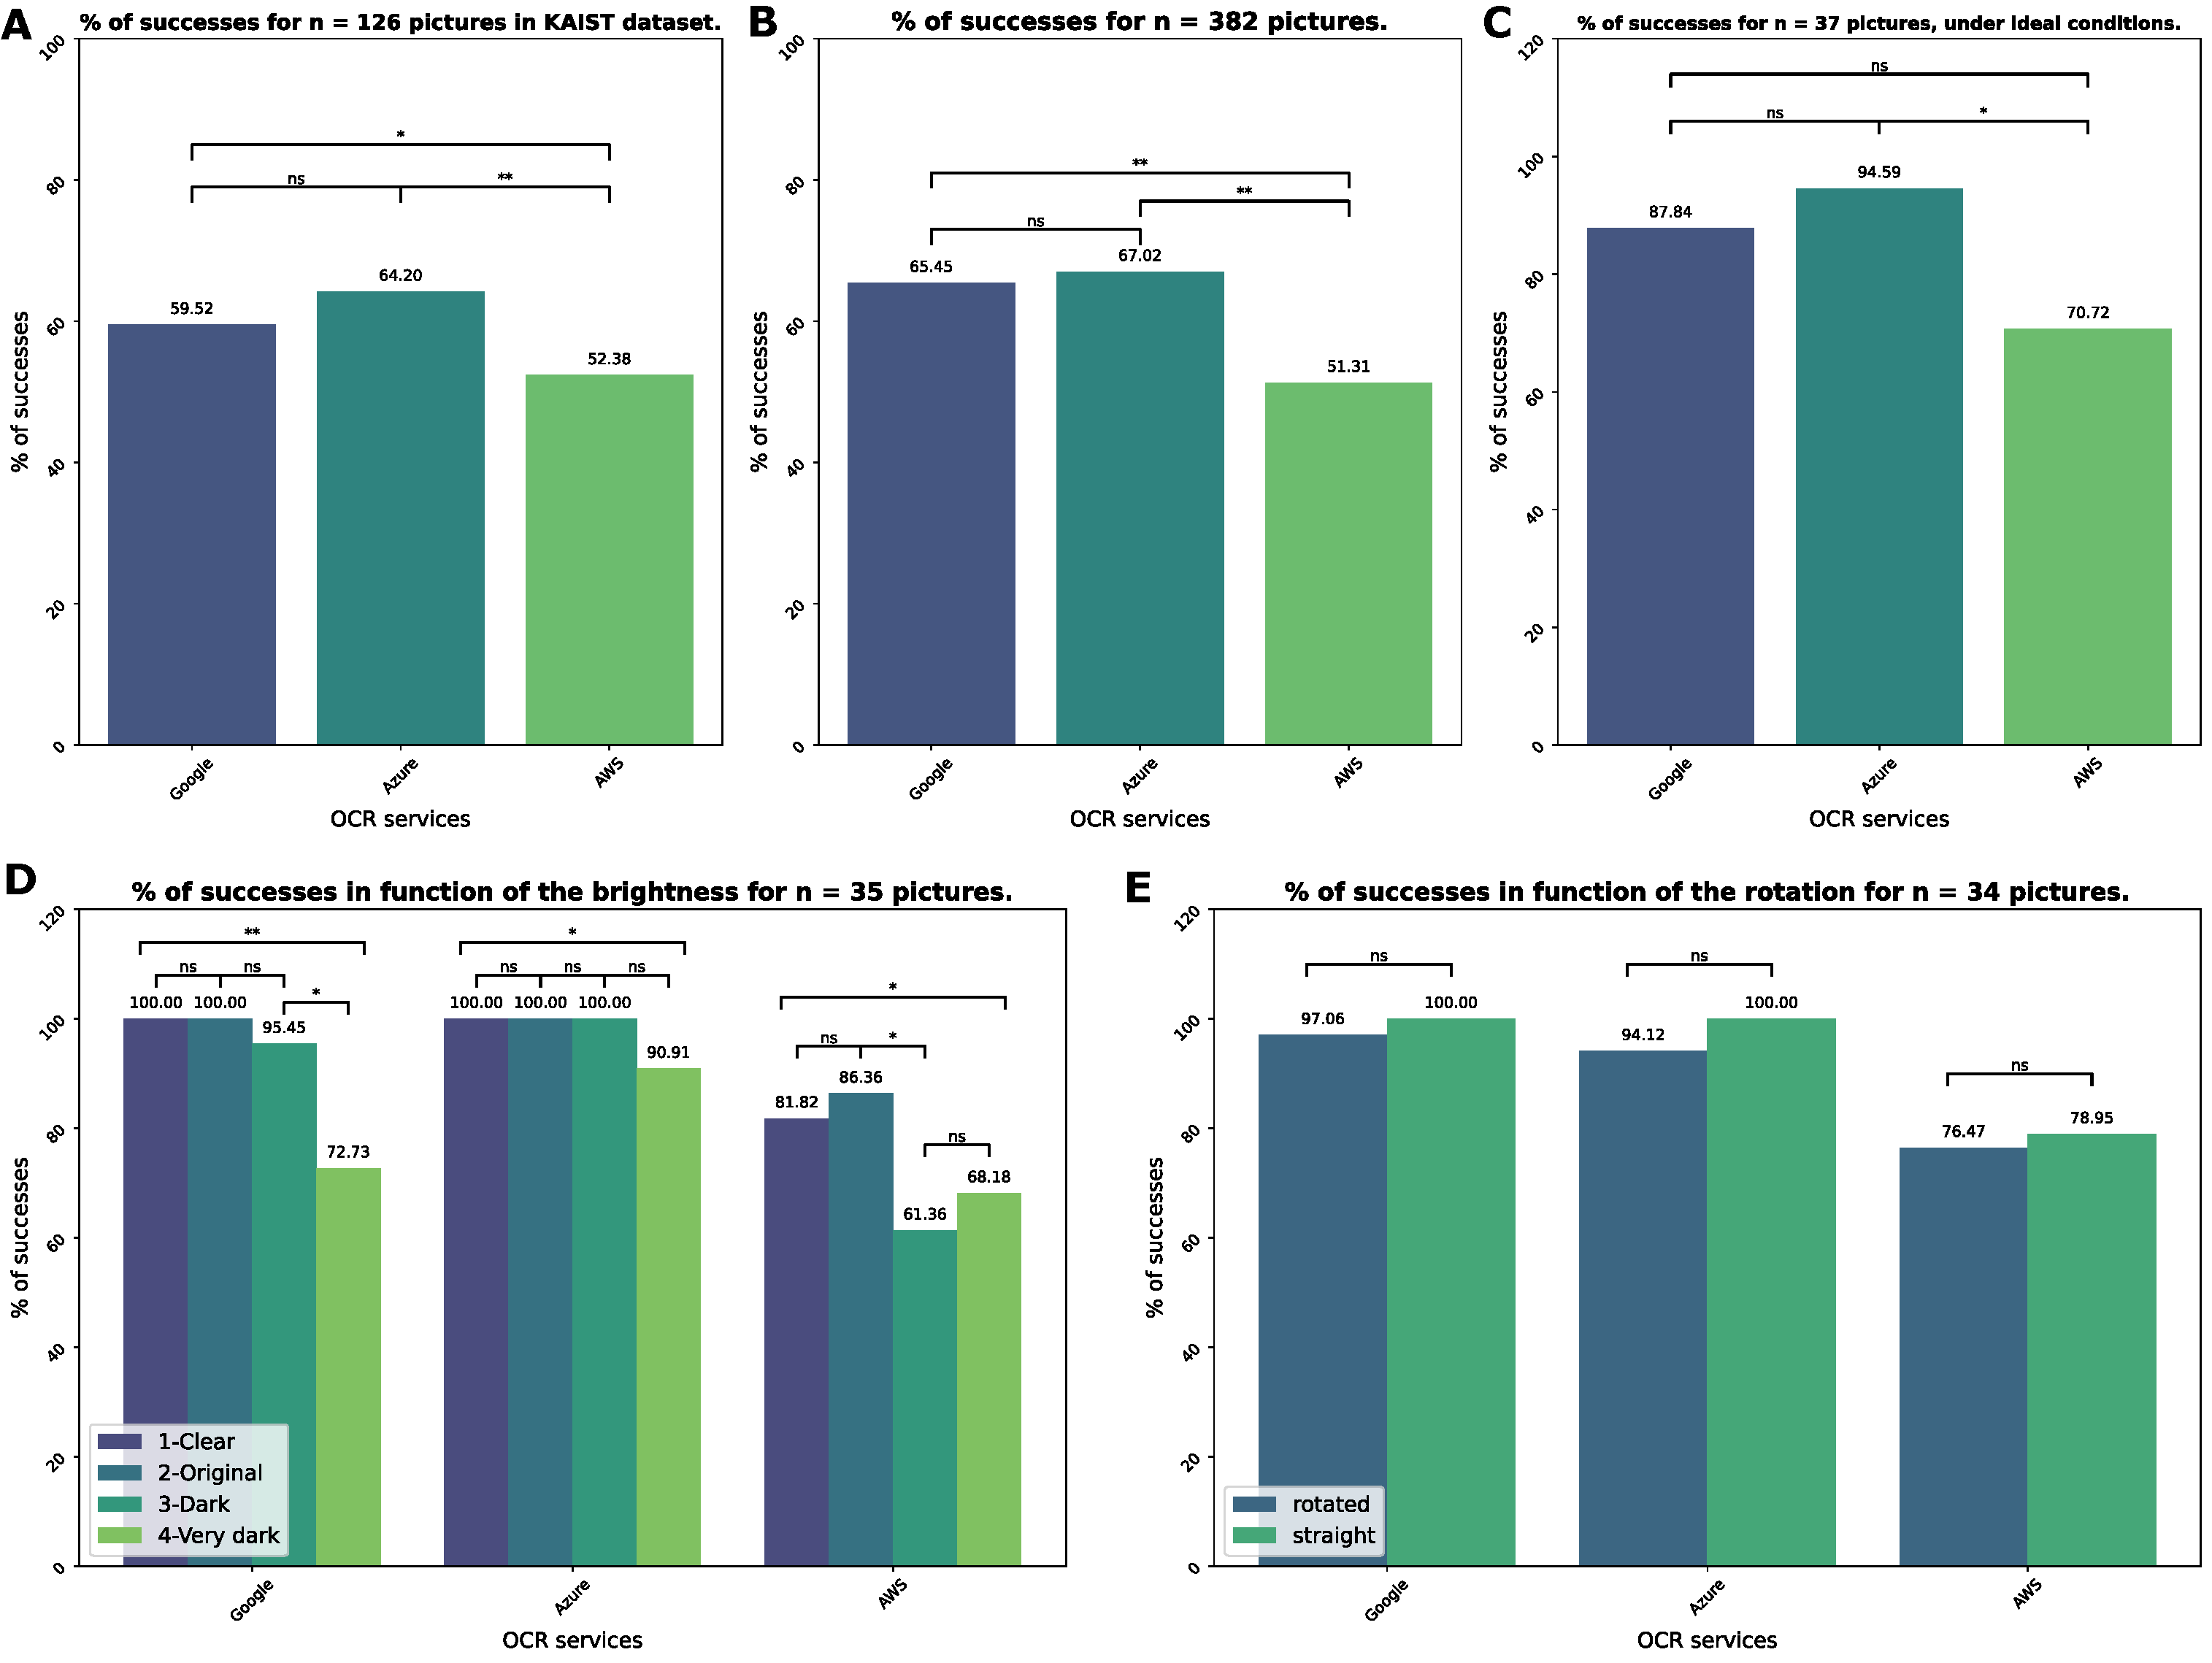
\includegraphics[width=0.9\textwidth]{figure/main_ocr.pdf}
 \caption{\textbf{Comparisons between Google Azure and AWS \gls{OCR} services, on uncurved text} \textbf{A)} Percentages of successes of the three OCRs on 126 pictures taken from an external data set: KAIST English scene text database \cite{KAIST}. \textbf{B)}
 Percentages of successes for 382 pictures of stamps [\textcolor{red}{Fig.}\ref{quality_cycle_sup}\textcolor{red}{-C}], with different cameras, orientation and lighting conditions. \textbf{C)} Percentages of successes for 37 "ideal" stamps pictures, \textit{ie} the objects have been placed in the center of the picture, straight in comparison of picture's frame, and with optimal lighting condition. \textbf{D)} Percentages of successes according pictures' brightness. To get comparable results pictures brightness as been processed adding the value 20 to all pixels of the 'Original' pictures for the 'Clear' condition, and removing respectively -30 and -50 for the 'Dark' and 'Very dark' conditions. \textbf{E)} Assessment of OCRs de-skew technique, photographing the objects with an angle between $\pm[60;120]$. For each comparison $\Chi_2$ independency tests have been realized, 'ns' implies that the hypothesis H0 cannot be rejected, '*' that H0 has been rejected under a risk $\alpha =0.05$, and '**' that H0 has been rejected under a risk $\alpha =0.01$.}
 \label{OCR_main}
\end{figure}
% ----------------------------------------------------------------------------------------------------------------------------------------------
\subsection{Comparison between of features extractor CNNs }
As introduced, the literature review led us to focus our study on faster \gls{R-CNN} model, since it appears to be the best technique in term of accuracy. We compared the last two published feature extractor networks, \textit{ie.} Inception-v2 and Inception-v4-Resnet-v2, that we will respectively called in this section inception and Resnet. Considering the same data set and the same training time, both models manage to learn the training data since the loss curves converge toward 0 [\textcolor{red}{Fig.}\ref{comp_inception_ResNet}\textcolor{red}{-A}]. Furthermore, both models don't suffer neither from over-fitting nor under-fitting, given the trend of the validation loss curves [\textcolor{red}{Fig.}\ref{comp_inception_ResNet}\textcolor{red}{-A}] and the proportions of successes that for each metric and for the two models which are not statistically different between the training and the validation sets [\textcolor{red}{Table.}\ref{Table_inception_resnet}]. Analyzing the main trands of the training [\textcolor{red}{Fig.}\ref{comp_inception_ResNet}\textcolor{red}{-A,B,C}] we noticed that Resnet outperforms Inception. Firstly according to the loss curves it appears that the training is faster and more stable with Resnet [\textcolor{red}{Fig.}\ref{comp_inception_ResNet}\textcolor{red}{-A}]. Resnet faster speed of convergence is also clearly visible on the \gls{mAP} validation curves [\textcolor{red}{Fig.}\ref{comp_inception_ResNet}\textcolor{red}{-B,C}]. Secondly, analyzing the mAP curves [\textcolor{red}{Fig.}\ref{comp_inception_ResNet}\textcolor{red}{-B}], it emerges that inception is more accurate with at the end of the training an \gls{mAP} equivalent to $\simeq 0.82$ against $\simeq 0.78$ for Inception. Thirdly, Resnet is more sensitive given the analysis of \gls{AR} curves which converge toward $\simeq 0.86$ against $\simeq 0.79$ for Inception [\textcolor{red}{Fig.}\ref{comp_inception_ResNet}\textcolor{red}{-C}]. These general analysis are confirmed by the comparisons of the proportions of successes between the two models, and especially by the comparison of the proportions of pictures correctly labeled, which is the most important metric, and that is significantly higher for the three sets with Resnet as features extractor network [\textcolor{red}{Table.}\ref{Table_inception_resnet}]. Analyzing, in detail the results on the the test set, we can point out that for the two models each screw label have been learned with the same rate of success [\textcolor{red}{Fig.}\ref{comp_inception_ResNet}\textcolor{red}{-D,F}], which demonstrate in one hand the homogeneity of the pictures between the test and the training set and in second hand the constant quality of pictures between the different screws. This also shows the ability of the model to learn character of different font-size since the results are similar between screw of different diameter. Finally, enumerating the different errors on the test, we can point out the very low number of failure in both cases [\textcolor{red}{Fig.}\ref{comp_inception_ResNet}\textcolor{red}{-E,G}], and secondly the excellent performances of Resnet knowing that the miss-classification of "4" to "x" results from labeling error, and that the false negative "/" an be explained by the presence of a scratch. Given this sum of information, we chose Inception-v4-Resnet-v2 as feature extractor network for its accuracy and its speed, to continue the training with others objects.
\begin{table}[H]
\scriptsize
\begin{tabular}{c|l|l|l|l|l|l|l|l|l|}
\cline{2-10}
\multicolumn{1}{l|}{}                       & \multicolumn{3}{c|}{\textbf{Train}}                                      & \multicolumn{3}{c|}{\textbf{Test}}                                      & \multicolumn{3}{c|}{\textbf{Validatition}}                             \\ \cline{2-10} 
\multicolumn{1}{l|}{}                       & \multicolumn{1}{c|}{Inception}             & \multicolumn{1}{c|}{Resnet}             & \multicolumn{1}{c|}{s} & \multicolumn{1}{c|}{Inception}            & \multicolumn{1}{c|}{Resnet}             & \multicolumn{1}{c|}{s} & \multicolumn{1}{c|}{Inception}            & \multicolumn{1}{c|}{Resnet}            & s \\ \hline
\multicolumn{1}{|c|}{\textbf{\begin{tabular}[c]{@{}c@{}}\% pictures \\ correctly\\ produced\end{tabular}}}  & \begin{tabular}[c]{@{}l@{}}$\frac{4992}{5190}$\\ $= 96.185\%$\end{tabular}  & \begin{tabular}[c]{@{}l@{}}$\frac{5188}{5190}$\\ $ = 99.942\%$\end{tabular} & *      & \begin{tabular}[c]{@{}l@{}}$\frac{1211}{1224}$\\ $ = 98.938\%$\end{tabular} & \begin{tabular}[c]{@{}l@{}}$\frac{1222}{1224}$\\ $ = 99.837\%$\end{tabular} & *      & \begin{tabular}[c]{@{}l@{}}$\frac{339}{348}$\\ $ = 97.414\%$\end{tabular} & \begin{tabular}[c]{@{}l@{}}$\frac{348}{348}$\\ $ = 100\%$\end{tabular} & * \\ \hline
\multicolumn{1}{|c|}{\textbf{\begin{tabular}[c]{@{}c@{}}\% bounding boxes\\ correctly predicted\end{tabular}}} & \begin{tabular}[c]{@{}l@{}}$\frac{49846}{50040}$\\ $ = 99.612\%$\end{tabular} & \begin{tabular}[c]{@{}l@{}}$\frac{50039}{50040}$\\ $ = 99.999\%$\end{tabular} & *      & \begin{tabular}[c]{@{}l@{}}$\frac{11764}{11775}$\\ $ = 99.966\%$\end{tabular} & \begin{tabular}[c]{@{}l@{}}$\frac{11775}{11775}$\\ $ = 100\%$\end{tabular} & NS      & \begin{tabular}[c]{@{}l@{}}$\frac{3367}{3375}$\\ $ = 99.763\%$\end{tabular} & \begin{tabular}[c]{@{}l@{}}$\frac{3375}{3375}$\\ $ = 100\%$\end{tabular} & * \\ \hline
\multicolumn{1}{|c|}{\textbf{\begin{tabular}[c]{@{}c@{}}\% characters \\ correctly predicted\end{tabular}}}  & \begin{tabular}[c]{@{}l@{}}$ \frac{49769}{ 50040}$\\ $ = 99.458\%$\end{tabular} & \begin{tabular}[c]{@{}l@{}}$\frac{50039}{50040}$\\ $ = 99.999\%$\end{tabular} & *      & \begin{tabular}[c]{@{}l@{}}$\frac{11763}{11775}$\\ $ = 99.989\%$\end{tabular} & \begin{tabular}[c]{@{}l@{}}$\frac{11773}{11775}$\\ $ = 99.992\%$\end{tabular} & NS      & \begin{tabular}[c]{@{}l@{}}$\frac{3366}{3375}$\\ $ = 99.763\%$\end{tabular} & \begin{tabular}[c]{@{}l@{}}$\frac{3375}{3375}$\\ $ = 100\%$\end{tabular} & * \\ \hline
\end{tabular}
\caption{ \textbf{Summary of the performances of faster \gls{R-CNN} with inception-v2 (referring to inception) and inception-v4-resnet-v2 (referring to resnet) as feature extractor CNN.} For the first row of comparisons a picture is said fully correctly predicted if all bounding boxes have been found and if each character correctly classify. The deviation between the proportion of bounding boxes correctly predicted and the proportion of characters correctly predicted comes from the characters successfully located but miss-classified. The "s" columns refer to the statistical significance of the unilateral proportion Z-tests under the null hypothesis (H0) that resnet perform better than inception, like this the "*" symbols imply that H0 have been rejected under the risk $\alpha = 0.05$ ans "NS" imply that the differences are not significant.}
\label{Table_inception_resnet}
\end{table}




\begin{figure}[H]
 \centering
 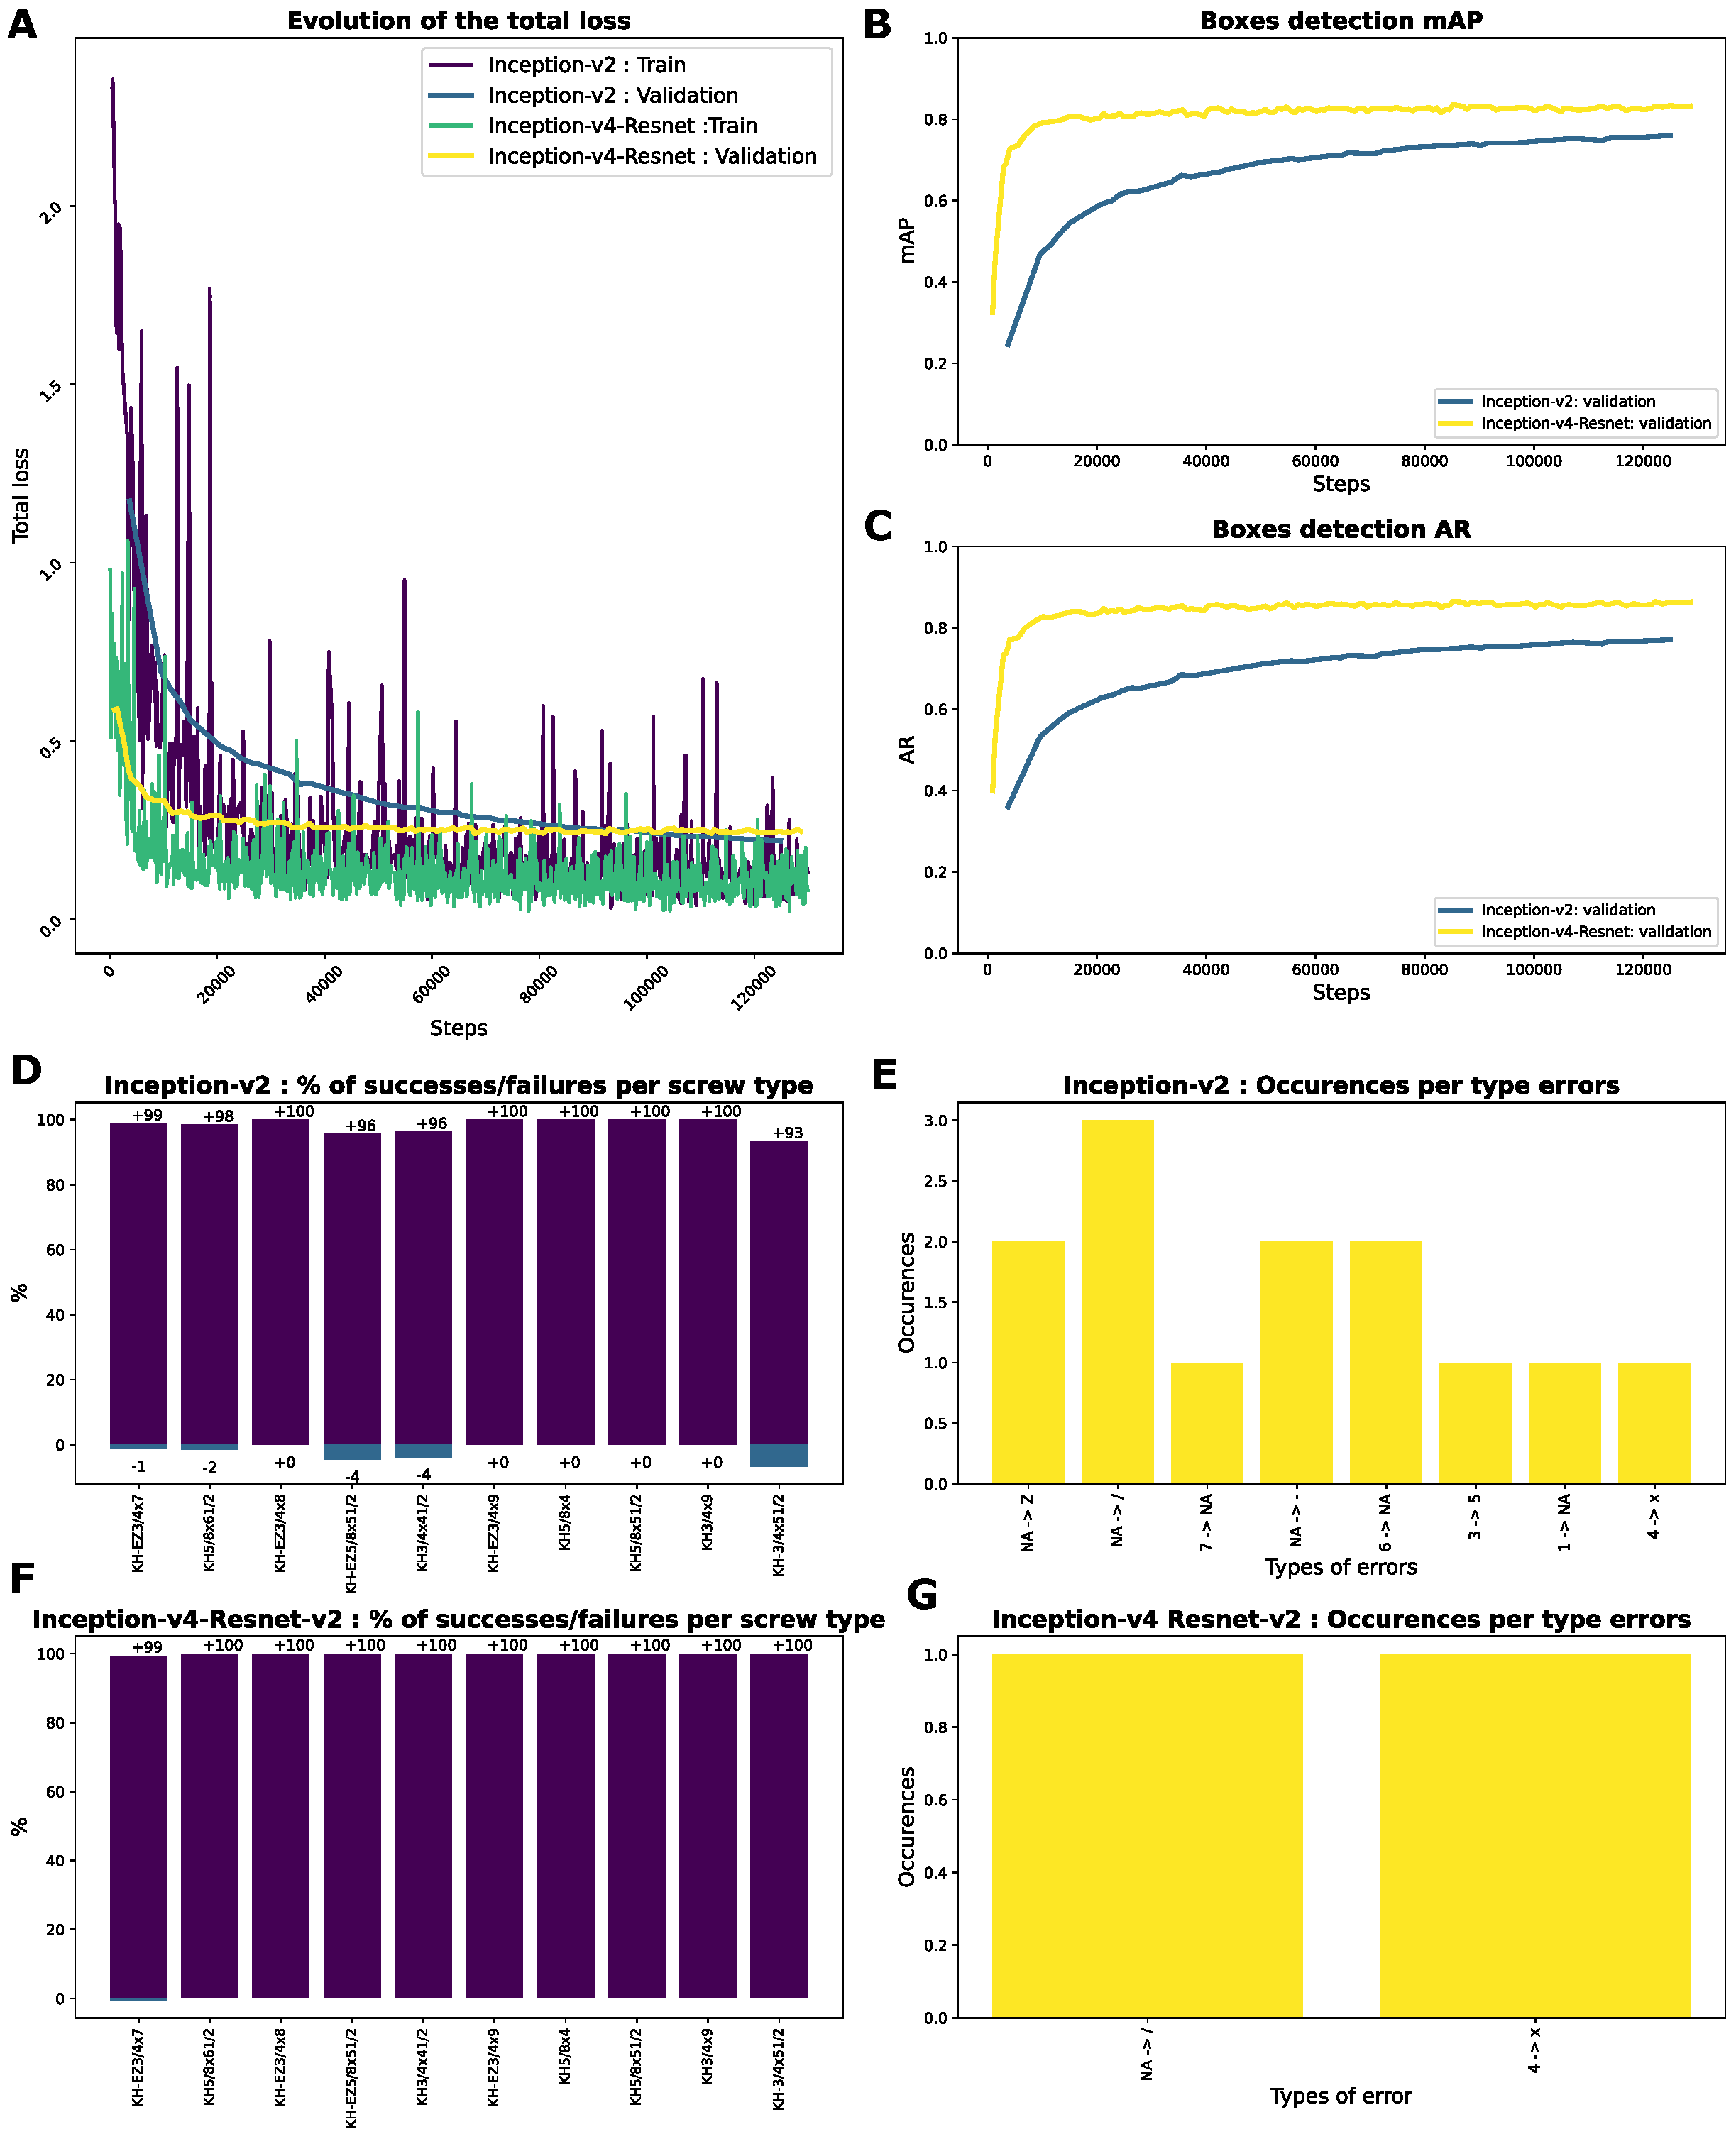
\includegraphics[width=0.82\textwidth]{figure/res_inception_resnet.pdf}
 \caption{\textbf{Comparaison of Inception-v2 and Inception-v4-ResNet-v2 as featuture extractors.} \textbf{A)} Evolution Total loss for the training set and the validation set with Inception-v2 and Inception-v4-ResNet-v2 as feature extractors. \textbf{B)} Box detection \gls{mAP} (mean average precision) for the validation sets according to the two feature extractors compared. The \gls{mAP} metric is the mean of the areas under the precision/recall curve for a given set of recall levels \cite{everingham2011pascal}. For recall, the precision is defined as (\gls{TP}/(\gls{TP}+\gls{FP})), and the recall as (\gls{TP}/(\gls{TP}+\gls{FN})). \textbf{C)} Average recall (\gls{AR}) for the validation sets according to the two feature extractors. The average recall is the value of integral of the recall over the \gls{IoU}. (\textit{The recall values are inversely proportional to the \gls{IoU} }). \textbf{D)} Proportions of pictures correctly and incorrectly predicted for the different types of screws with inception-v2 as a feature extractor. In the \gls{UI}, the screws of diameter $1/2$ have been excluded. The high level of errors observed associated with the screw labeled "KH-EZ 5/8 x3 1/2" can be considered an outlier values because of picture quality. \textbf{E)} Occurrences of all types of errors, with inception-v2 as a feature extractor. $x \rightarrow \text{NA}$ corresponds to of \gls{FN}, whereas $x$ must have been detected, $ \text{NA} \rightarrow x$ corresponds to of \gls{FP}, whereas $x$ must not have been detected, $x_1 \rightarrow x_2$ corresponds to a miss-classification of the $x_2$ that must have been detected as $x_1$. \textbf{F)} and \textbf{G)} are the same as \textbf{(D)} and respectively \textbf{(E)} with Inception-v4-ResNet-v2 as a feature extractor.}
 \label{comp_inception_ResNet}
\end{figure}

%% ______________________________GUI
\subsection{Application: "Hilti Fast Falcon"}
The application "Hilti Fast Falcon" is the final "product" of our case study. It have been implemented to work on the production line computers which are plugged to cameras and connected to a remote server, which is the \gls{GPU}. When the application is loaded, users have to first select the type of analysis, \textit{ie} screw or stamp analysis [\textcolor{red}{Fig.}\ref{app_view_success}\textcolor{red}{-1}]. Then, he/she scans the bar code associated to the purchase order being produced [\textcolor{red}{Fig.}\ref{app_view_success}\textcolor{red}{-2}]. If this one is readable it automatically completed the material number field [\textcolor{red}{Fig.}\ref{app_view_success}\textcolor{red}{-3}]. The expected label associated to this material number is then searched into Eilebrech data base. The expected label is returned only if it corresponds to a material number associated to screw of diameter $3/4$ or $5/8$ inches, or to linear stamps [\textcolor{red}{Fig.}\ref{MVC_SCA}\textcolor{red}{-Grey boxes}]. Once the object is correctly lighting and placed under the lens the user takes a picture [\textcolor{red}{Fig.}\ref{app_view_success}\textcolor{red}{-4}]. If the camera is not recognize, a picture locally stored on the computer can be loaded. The picture to analysis is display on the \gls{GUI} and also the expected label. If the client socket is open these information are send to the server [\textcolor{red}{Fig.}\ref{Seqenc_diagram}\textcolor{red}{-step 13}]. At this stage we assume that the model have been initialized, \textit{ie} the tensor flow session is open and the frozen graph has been loaded. If it is not the case only the stamps analysis program is available. The request is finally sent to queue of screw or stamp picture to [\textcolor{red}{Fig.}\ref{Seqenc_diagram}\textcolor{red}{-step 14}]. \textbf{If the analysis concerns a stamp picture}, this one is loaded into Azure OCR API \cite{AzureOCR}), the text predicted is then stored into a queue of analysis to post-process \textcolor{red}{Fig.}\ref{app_view_stamp_echec},\ref{app_view_stamp_sucess} \textcolor{red}]. The post processing protocol includes the comparison between the expected label and the predicted one, if it is a match the result returned is only a boolean such as \verb|success == True| otherwise the predicted label is align against the expected one through the Needleman and Wunsch's algorithm \cite{spr1970general}, and the results returned are then a Boolean turned to false, and the HTML code of the alignment where the miss-classification are indicating by red letters and the \gls{FN} by underscores [\textcolor{red}{Fig.}\ref{Seqenc_diagram}\textcolor{red}{-second Alt frame} ; \textcolor{red}{Fig.}\ref{app_view_stamp_echec}]. The post-processed results are added to a queue of results to send to the clients. After receiving the results the client communicate with the interface, which itself asks to the \gls{GUI} to display the prediction. \textbf{If the request concerns a screw} then it is handled by the Tensorflow model. In this case the accuracies of the bounding boxes detected are analyzed, \textit{ie} if the accuracy associated to a character is too low the coordinates of this object are stored into a dictionary. If any potential error has been detected, the results are directly sent to the queue of analysis to post process). The post-processing pipeline of screw pictures has a step upstream step to the text comparison which is the organization of the bounding boxes [\textcolor{red}{Fig.}\ref{blind}]. The following post-processing steps are identical to the ones described for the stamps. If one or several bounding boxes are suspected to be wrong intermediate steps between the prediction and the post processing pipeline involving the user are needed [\textcolor{red}{Fig.}\ref{Seqenc_diagram}\textcolor{red}{-first Alt frame} ; \textcolor{red}{Fig.}\ref{app_view_alt}]. For each potential wrong bounding box the user has to accept or reject the proposal [\textcolor{red}{Fig.}\ref{Seqenc_diagram}\textcolor{red}{-frame loop}]. A vector of bounding boxes to delete is then send to the server. The analysis is therefore ready to be post-processed, once the bounding boxes rejected have been deleted. Once the post-processing is done the results are returned and then displayed on the \gls{GUI}, contrary to the stamp case if the analysis didn't led to match the labeled pictured showing the bounding boxes is shown \textcolor{red}{Fig.}\ref{app_view_echec}]. To guarantee simultaneous client connections, each object stored is associated with a pointer toward the client socket object. This architecture allows guarantying a answer in 3 seconds in the best case \textit{ie} match between the expected and the predicted label [\textcolor{red}{Fig.}\ref{app_view_success} ;\ref{app_view_stamp_sucess}]. \textbf{This is an important improvement comparing to previous local version of the application, since using the production line computer one analysis took around 24 seconds}. It also eases the stamp analysis since computers on the production line does not have an access to internet [\textcolor{red}{Fig.}\ref{app_view_stamp_sucess} ; \ref{app_view_stamp_echec}]. Finally, this set up also optimizes the access to the GPU computational resources, since the multi-threading allows predicting a new picture while another analysis is being post-processed, the results of another are being sent to a client and a new request is being accepted by the server... If the server is not functional all the processes happen locally. For more details on the architecture Model-Controller-View Client/Server architecture you can refers to the UML diagram in annex 
[\textcolor{red}{Fig.}\ref{MVC_SCA}\textcolor{red}]

\begin{figure}[H]
 \centering
 \begin{subfigure}{0.6\textwidth}
  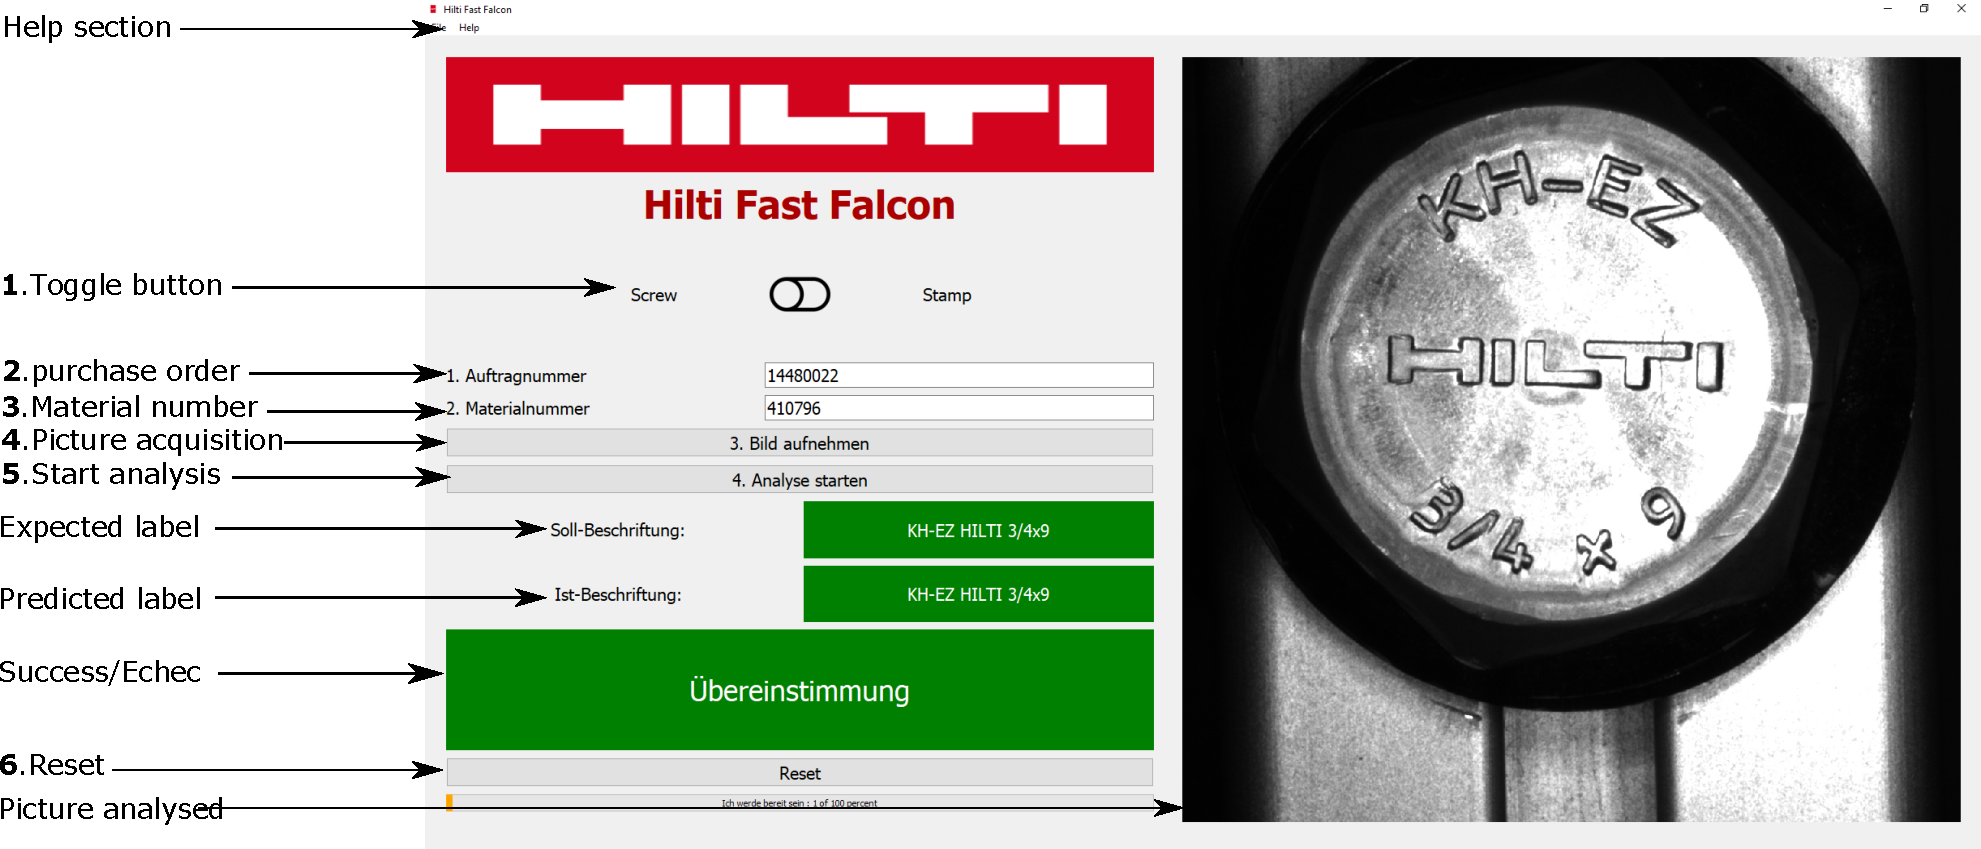
\includegraphics[width=\linewidth]{figure/APP_MAIN_A.pdf}
  \subcaption{}
  \label{app_view_success}
 \end{subfigure}
  \begin{subfigure}{0.6\textwidth}
  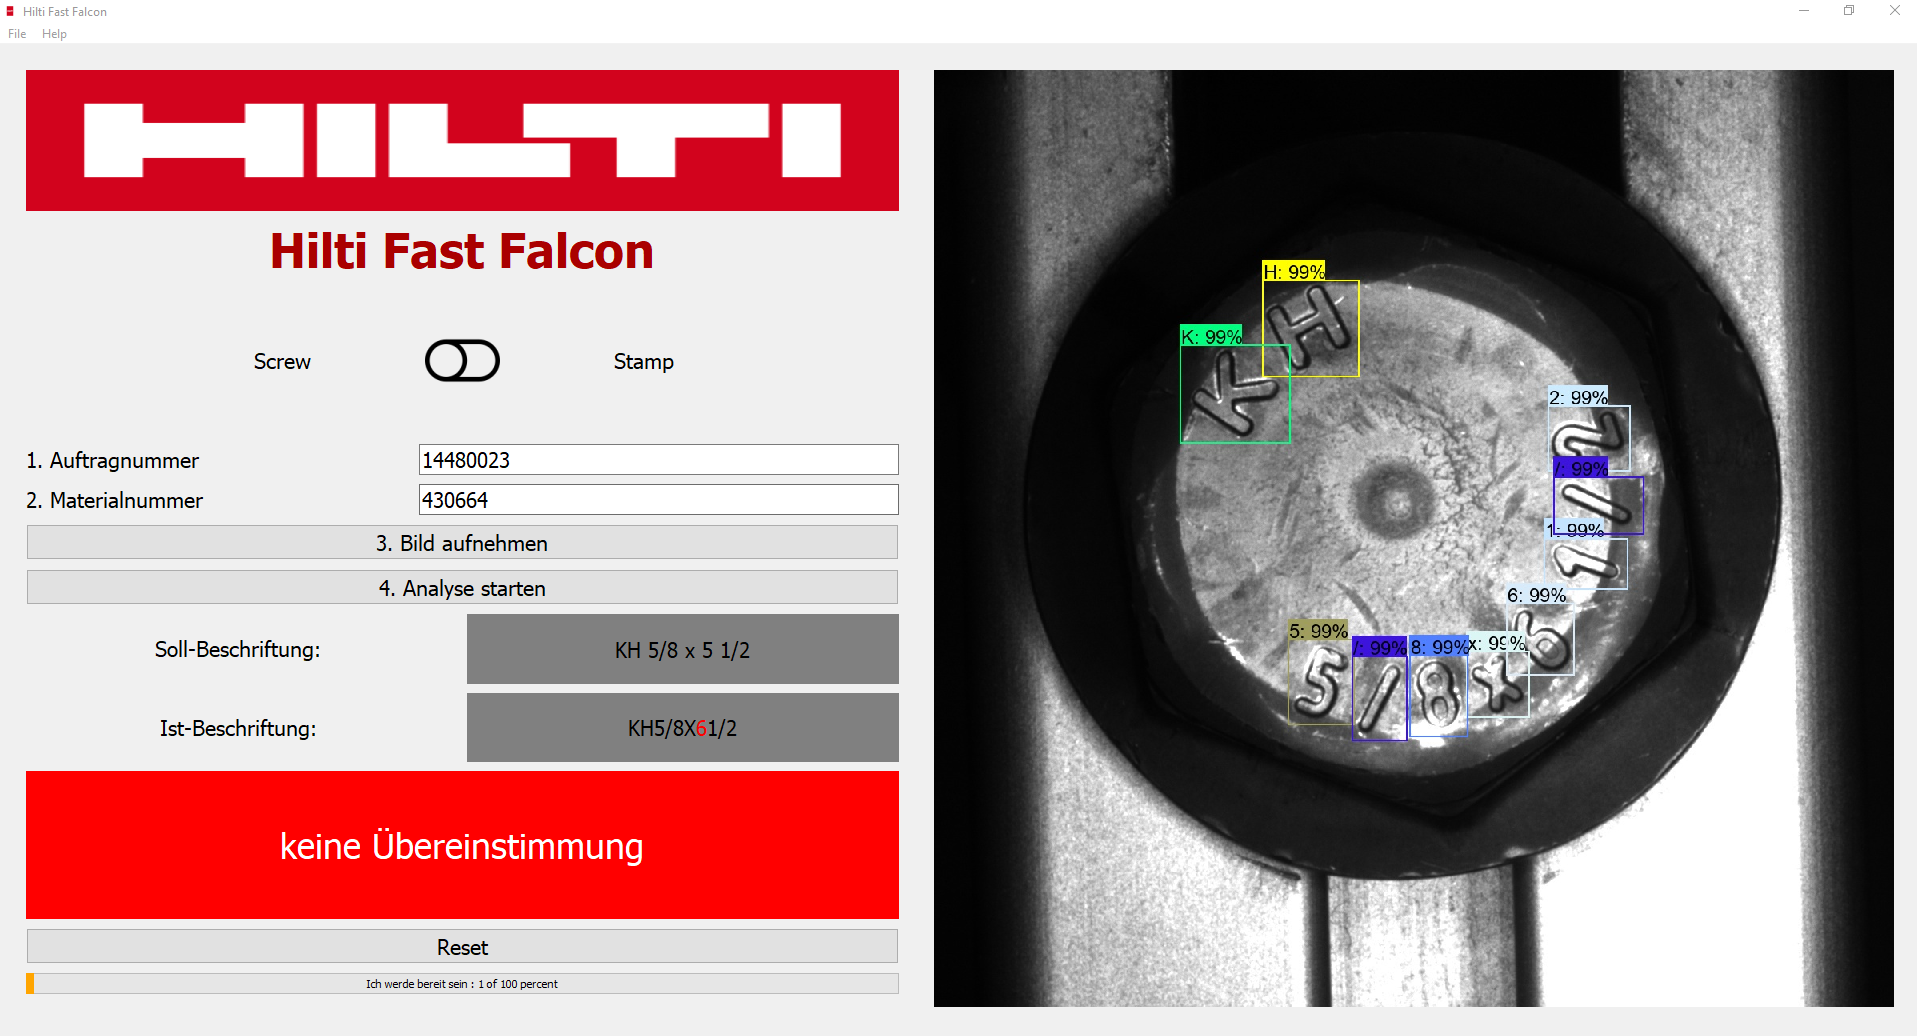
\includegraphics[width=\linewidth]{figure/screw_echec_APP_MAIN.png}
  \subcaption{}
  \label{app_view_echec}
 \end{subfigure}
 \caption{\textbf{Global views of the application} \textbf{A)} Presentation of the different functionalities and description of a screw's picture analysis that led to a match between the expected and the predicted label. \textbf{B)} Screw's picture analysis that led to a mismatch, in this case the labeled picture and the best alignment resulting from Needleman and Wunsch algorithm for predicted label are shown.}
 \label{APP_MAIN}
\end{figure}%



\begin{figure}[H]
 \centering
  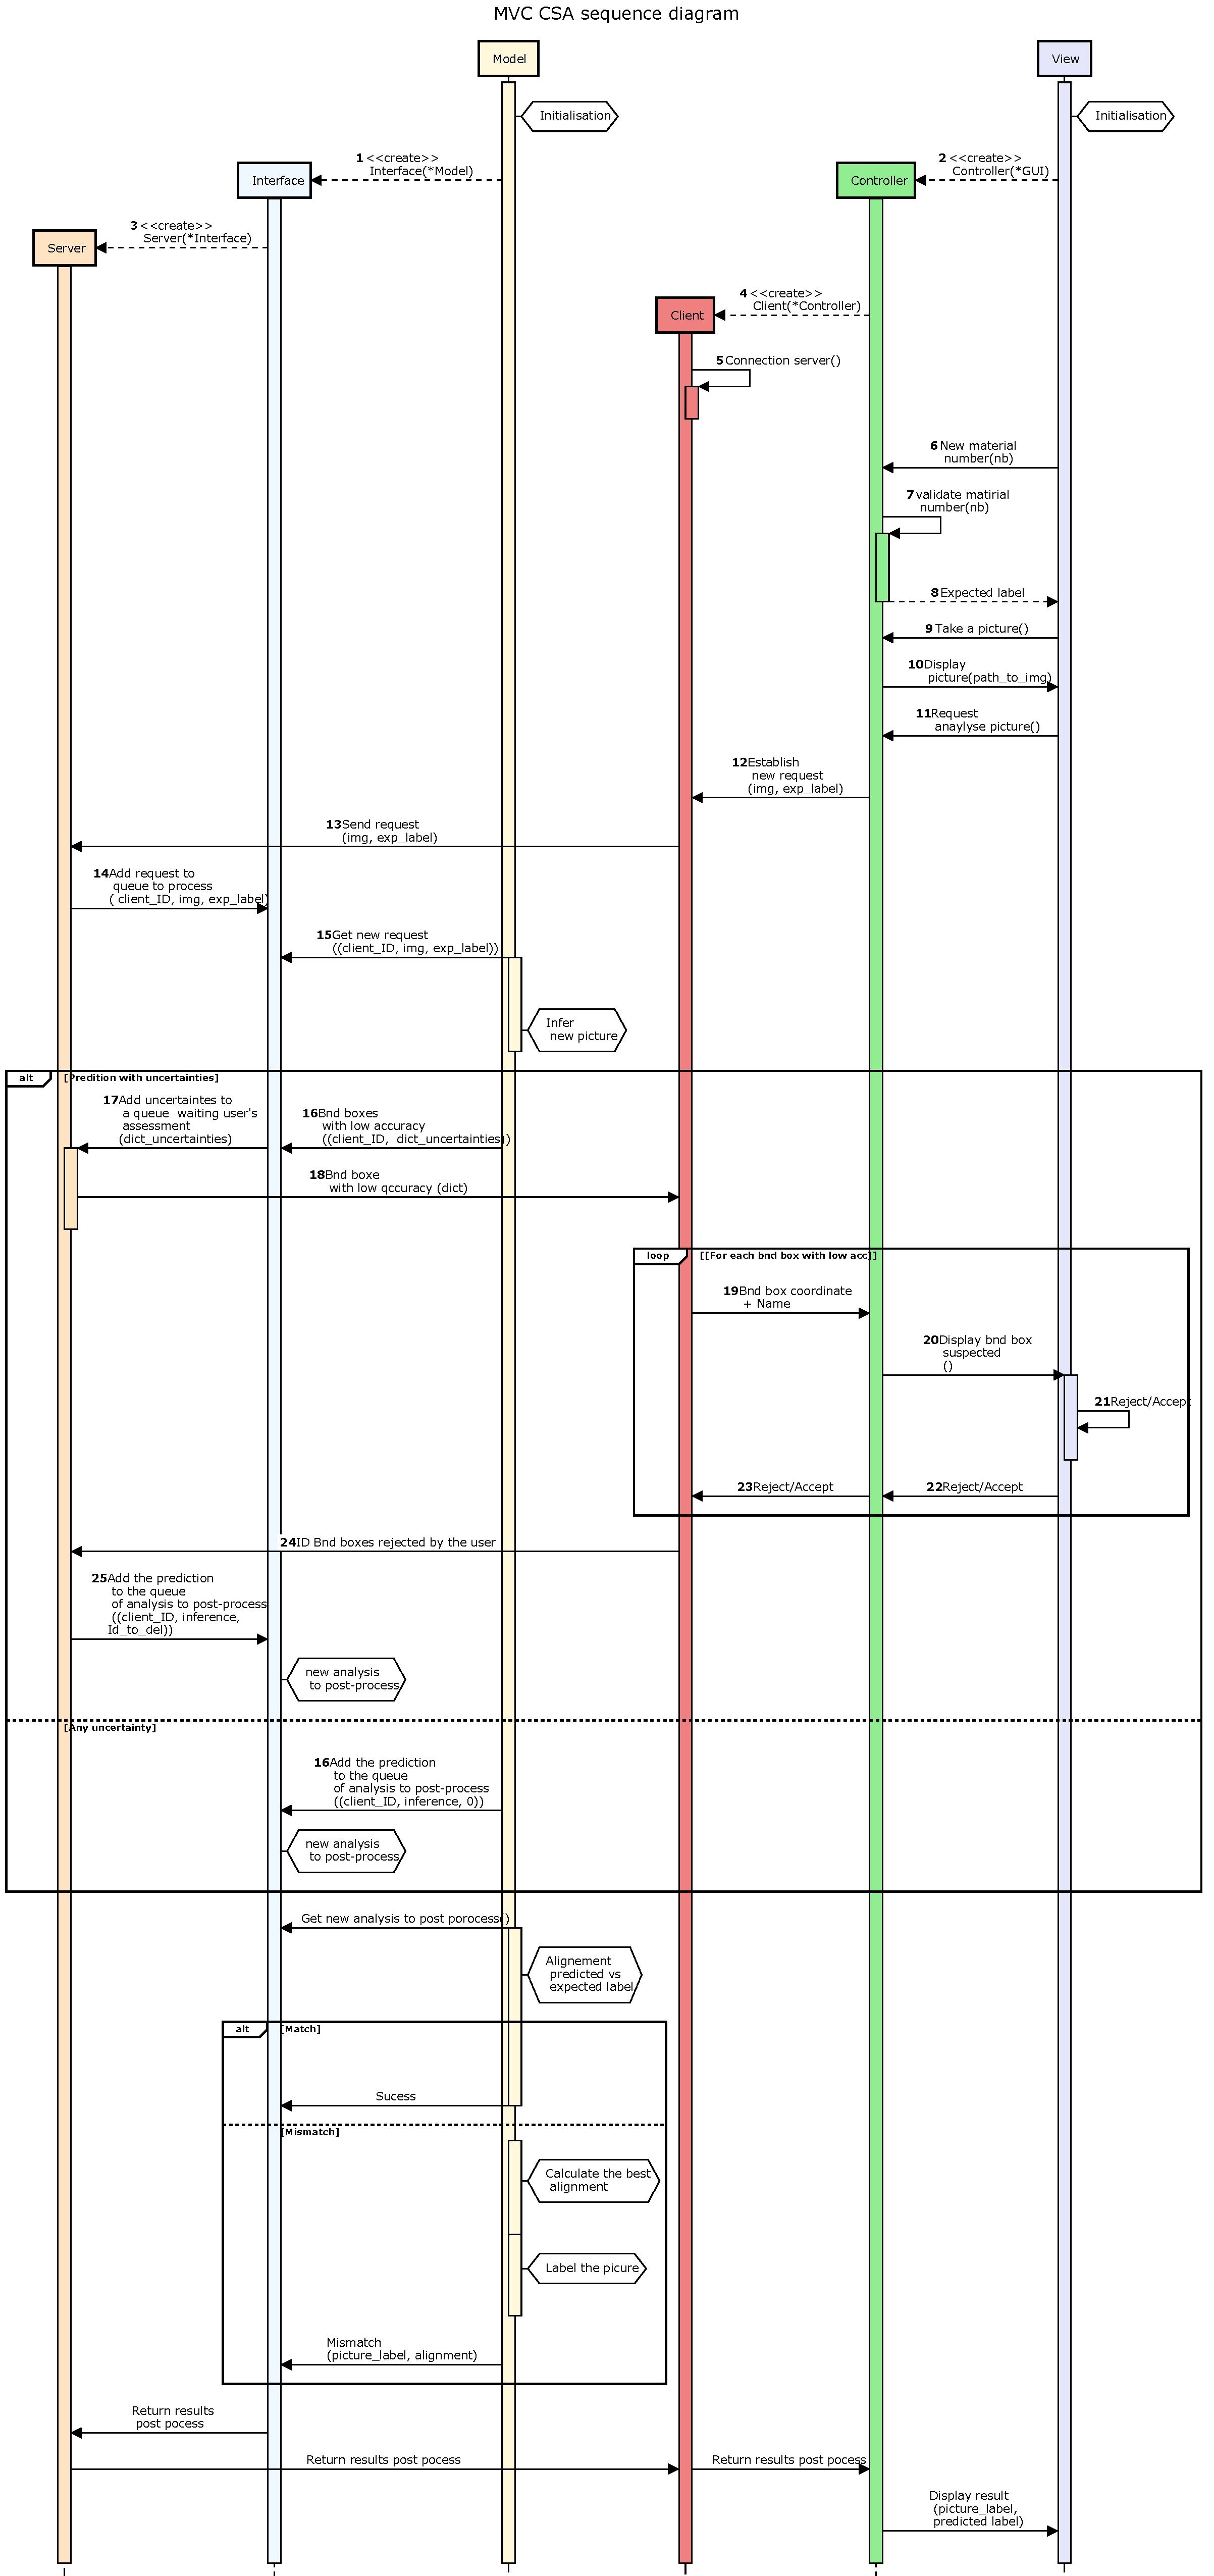
\includegraphics[width=0.8\textwidth, height=1\textheight]{figure/sequence_diagram.pdf}
  \clearpage 
  \vspace{-.7cm}
  \caption{}
 \label{Seqenc_diagram}
\end{figure}
\begin{figure}[t]
 \contcaption{ \textbf{Sequence diagram \gls{MVC} Client Server architecture} This diagram summarizes the interactions between the \gls{GUI} (violet boxes), the Controller (Green boxes) which is linked to the Client (Red boxes) if the Server (Oranges boxes) is connected. User's requests are handled by the Controller that through the Client send them to the Server, which is linked to the Interface (Blue boxes). The Interface copes with requests' order and send them to the Model (Yellow boxes). Firstly, the Model handles picture prediction. If the prediction contains potential mistakes, the bounding boxes associated to a low accuracy are send to the user, that have for each of them have to accept or reject the proposal (alt and loop). The ID bounding boxes rejected are then sent back to the Server that send a request to the interface to post-process the current analysis. The post-processed results are finally displayed on the \gls{GUI}. If any bounding box is considered as a potential error, the prediction is directly post-processed, before that the final results are displayed on the GUI.}% Continued caption
\end{figure}



\newpage
\section{Discussion}


%-----------------------------------------------------------------------------------
% Literature review
%----------------------------------------------------------------------------------------
\newpage


\begin{multicols}{2}
{\small
\bibliography{literature.bib} % Add the filename of your bibliography
\bibliographystyle{unsrt}
} % Defines your bibliography style
\end{multicols}
% For citing, please see this sheet: http://merkel.texture.rocks/Latex/natbib.php


\newpage
\small
\printglossaries

 
 
\newpage
\section{Supplementary figures}
\setcounter{figure}{0}
\setcounter{table}{0}
\makeatletter 
\renewcommand{\thefigure}{S\arabic{figure}}
\renewcommand{\thetable}{S\arabic{table}}

 \begin{figure}[H]
 \centering
 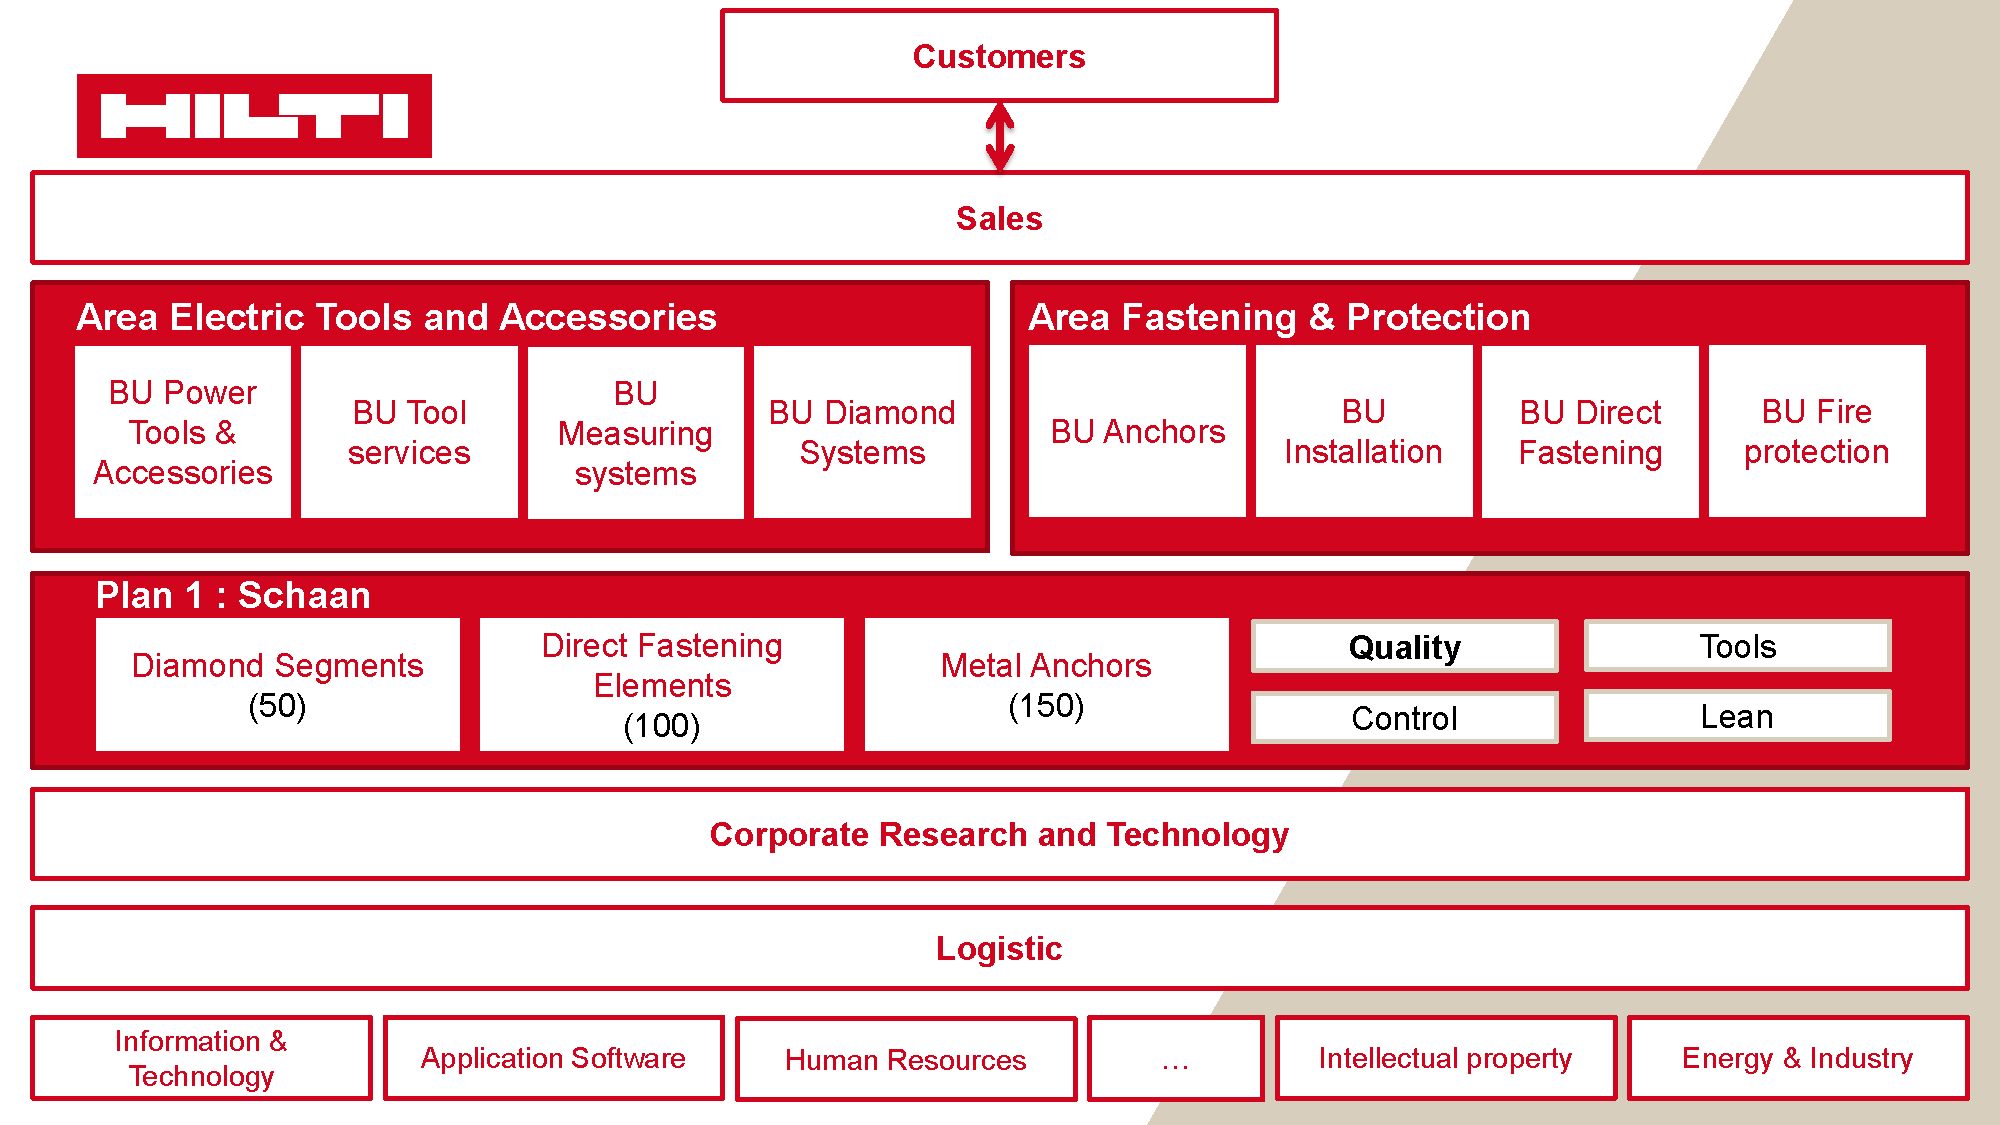
\includegraphics[width=0.8\textwidth]{figure/Hilti_organisation.pdf}
 \caption{\textbf{Organisation of Hilti Schaan} Diagram presenting the main department and their interactions.}
 \label{fig1_Hilti_organization}
\end{figure} 

\begin{figure}[H]
 \centering
 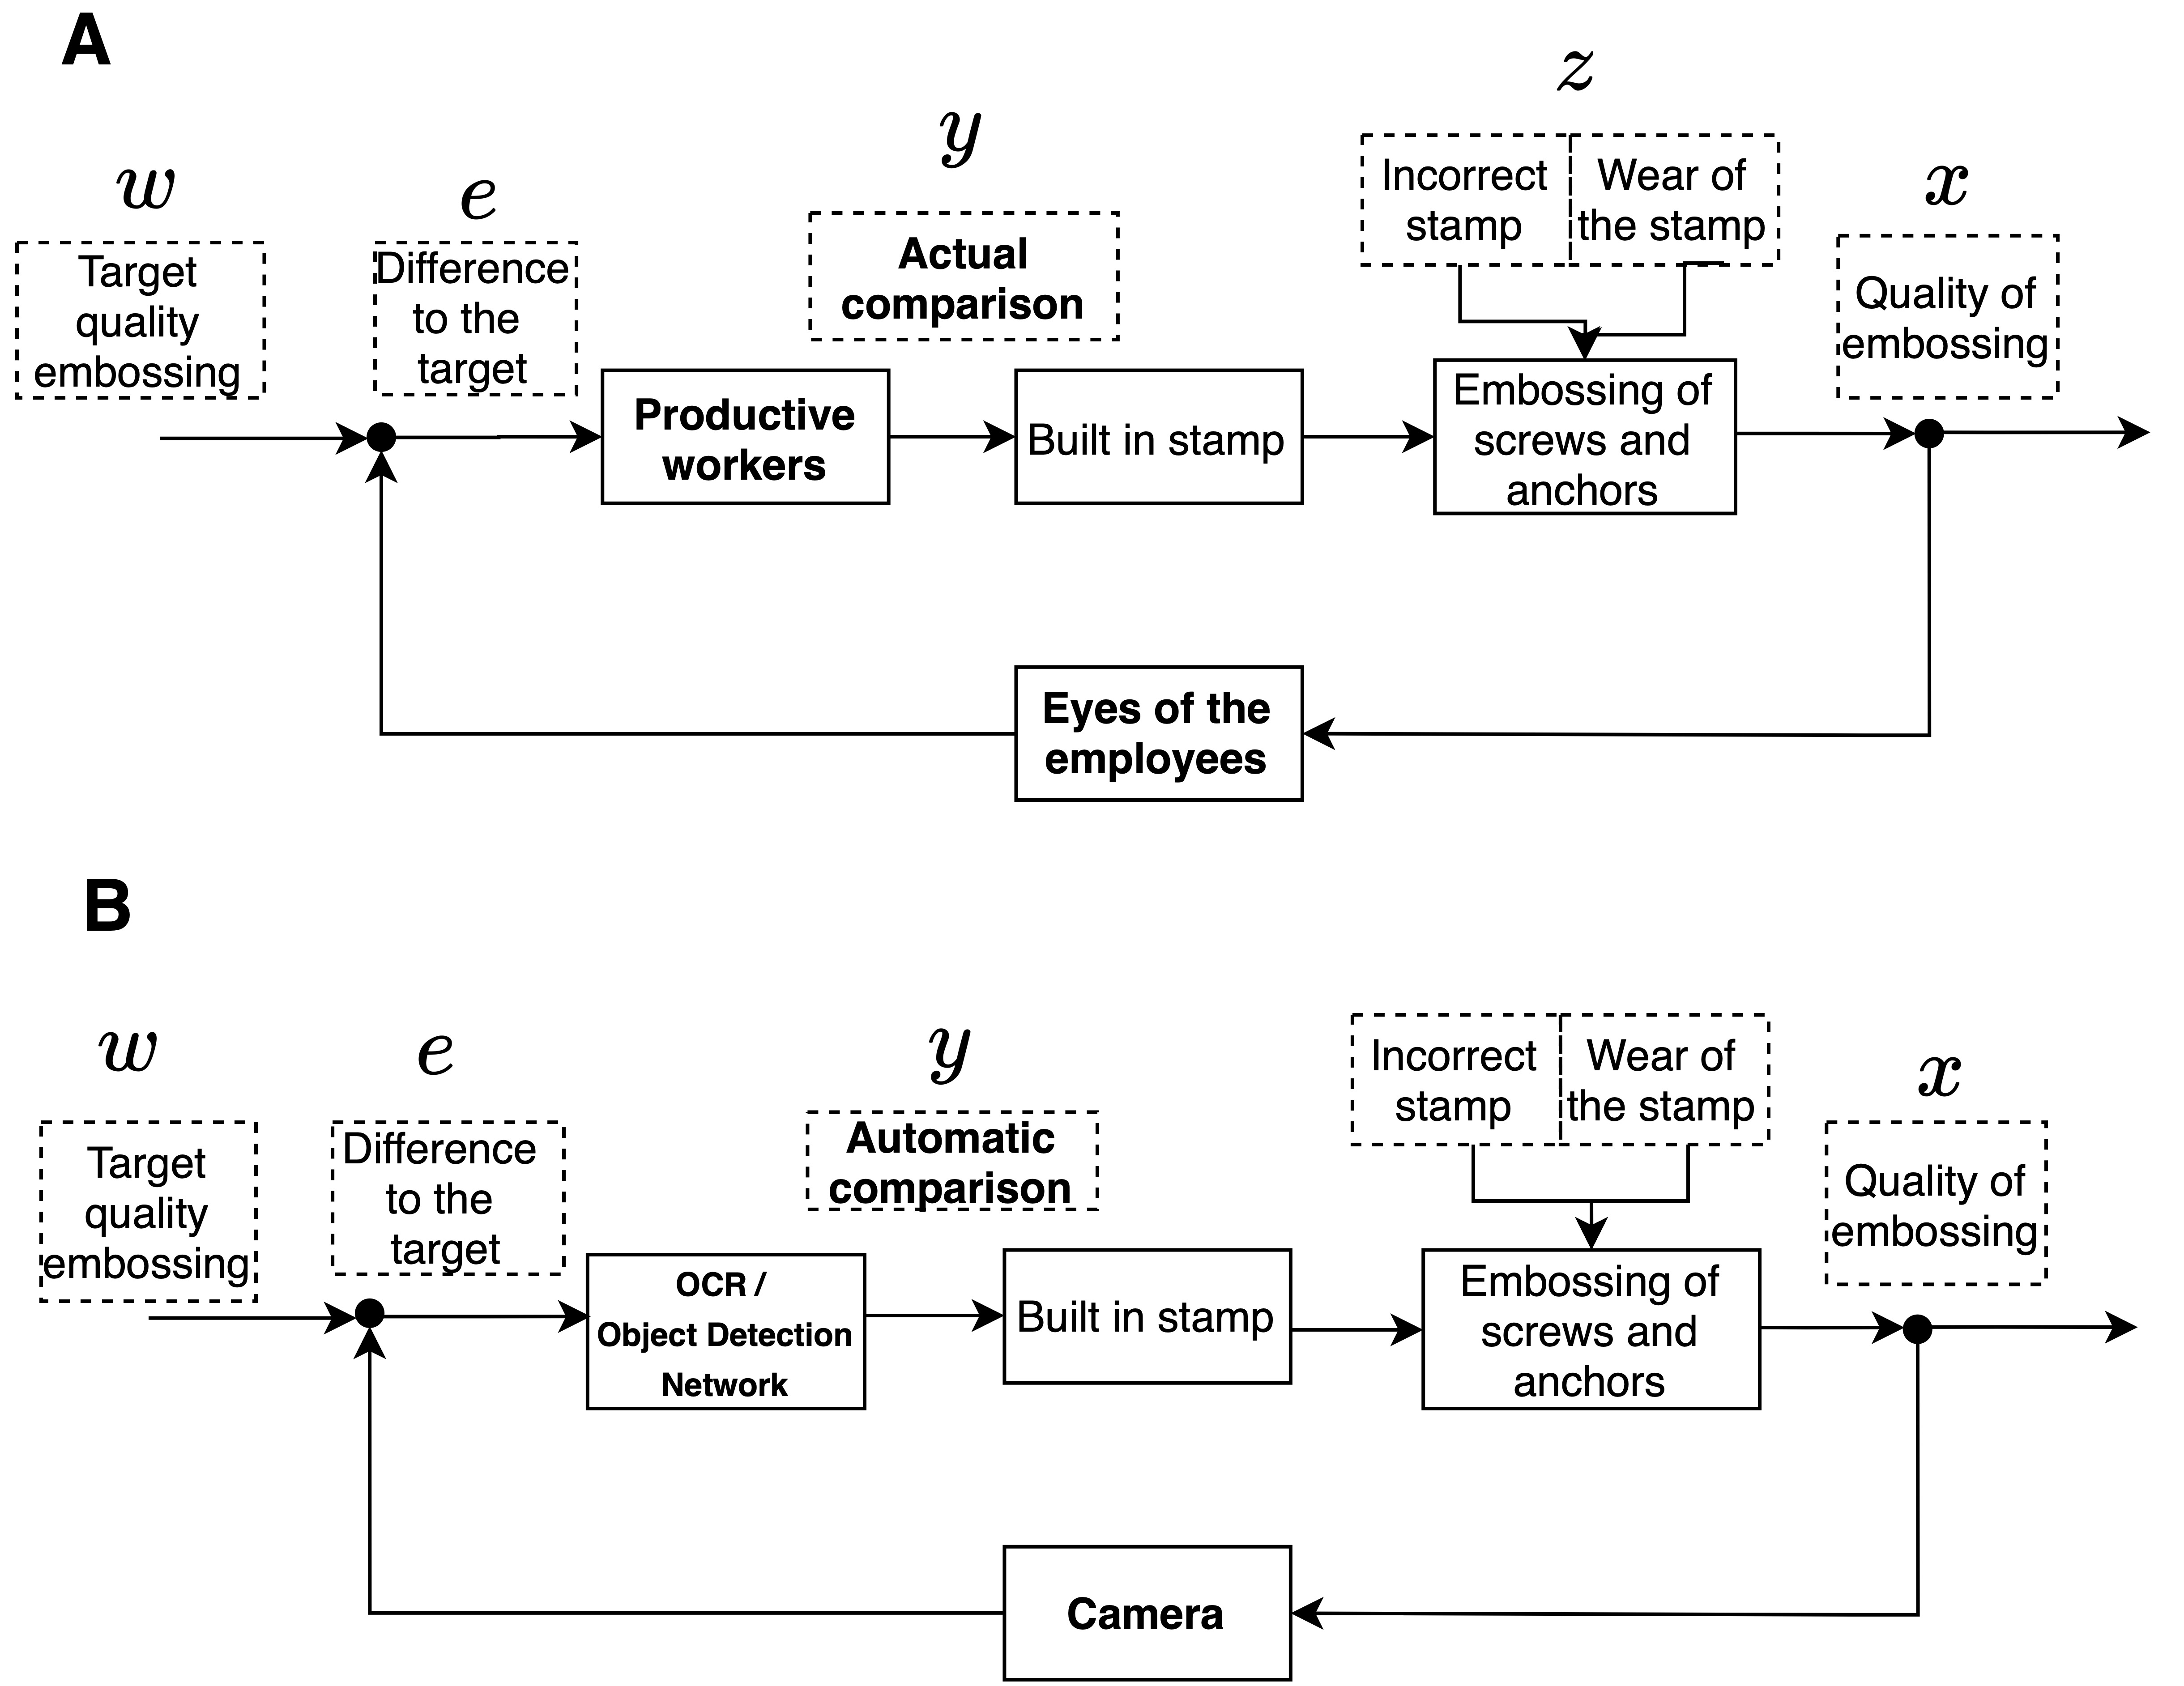
\includegraphics[width=0.8\textwidth]{figure/quality_cyle_sup.jpg}
 \caption{\textbf{Quality control cycles.} \textbf{A)} Current quality control cycle of embossing quality by visual control. \textbf{B)} Quality control cycle in implementation by computer vison.}
 \label{quality_cycle_sup}
\end{figure}




\begin{figure}[H]
 \centering
 \includegraphics[width=0.9\textwidth]{figure/blin4.jpg}
 \caption{\textbf{Comparison between the expected and predicted text.} The first column presents the tree clusters with in blue the cluster of letters, in red the cluster of numbers and in green the logo's cluster. In the first case, they are horizontally orientated, and in two following cases they are vertically orientated. The characters circled define the linking chain extremity, and the yellow arrow the reading direction expected. The second column presents the bounding boxes predicted. The third one the three linking chain. The last column present the two alignments resulting from Needleman and Wunsch \cite{spr1970general} algorithm, with yellow background the one resulting from the reversion of the linking chains. Finally, The final alignment retained are circled in green.}
 \label{blind}
\end{figure}

\begin{figure}[H]
 \centering
 \includegraphics[width=0.9\textwidth]{figure/screw_pipeline.jpg}
 \caption{\textbf{Assessment of OCR services performances on screw pre-processed pictures.}\textbf{A)} Pre-processing pipeline. \textbf{B)} Percentages of successes for each \gls{OCR} assessed on 33 pictures pre-processed according to the pipeline described. }
 \label{screw_pipeline}
\end{figure}


\begin{figure}[H]
 \centering
 \begin{subfigure}{0.6\textwidth}
  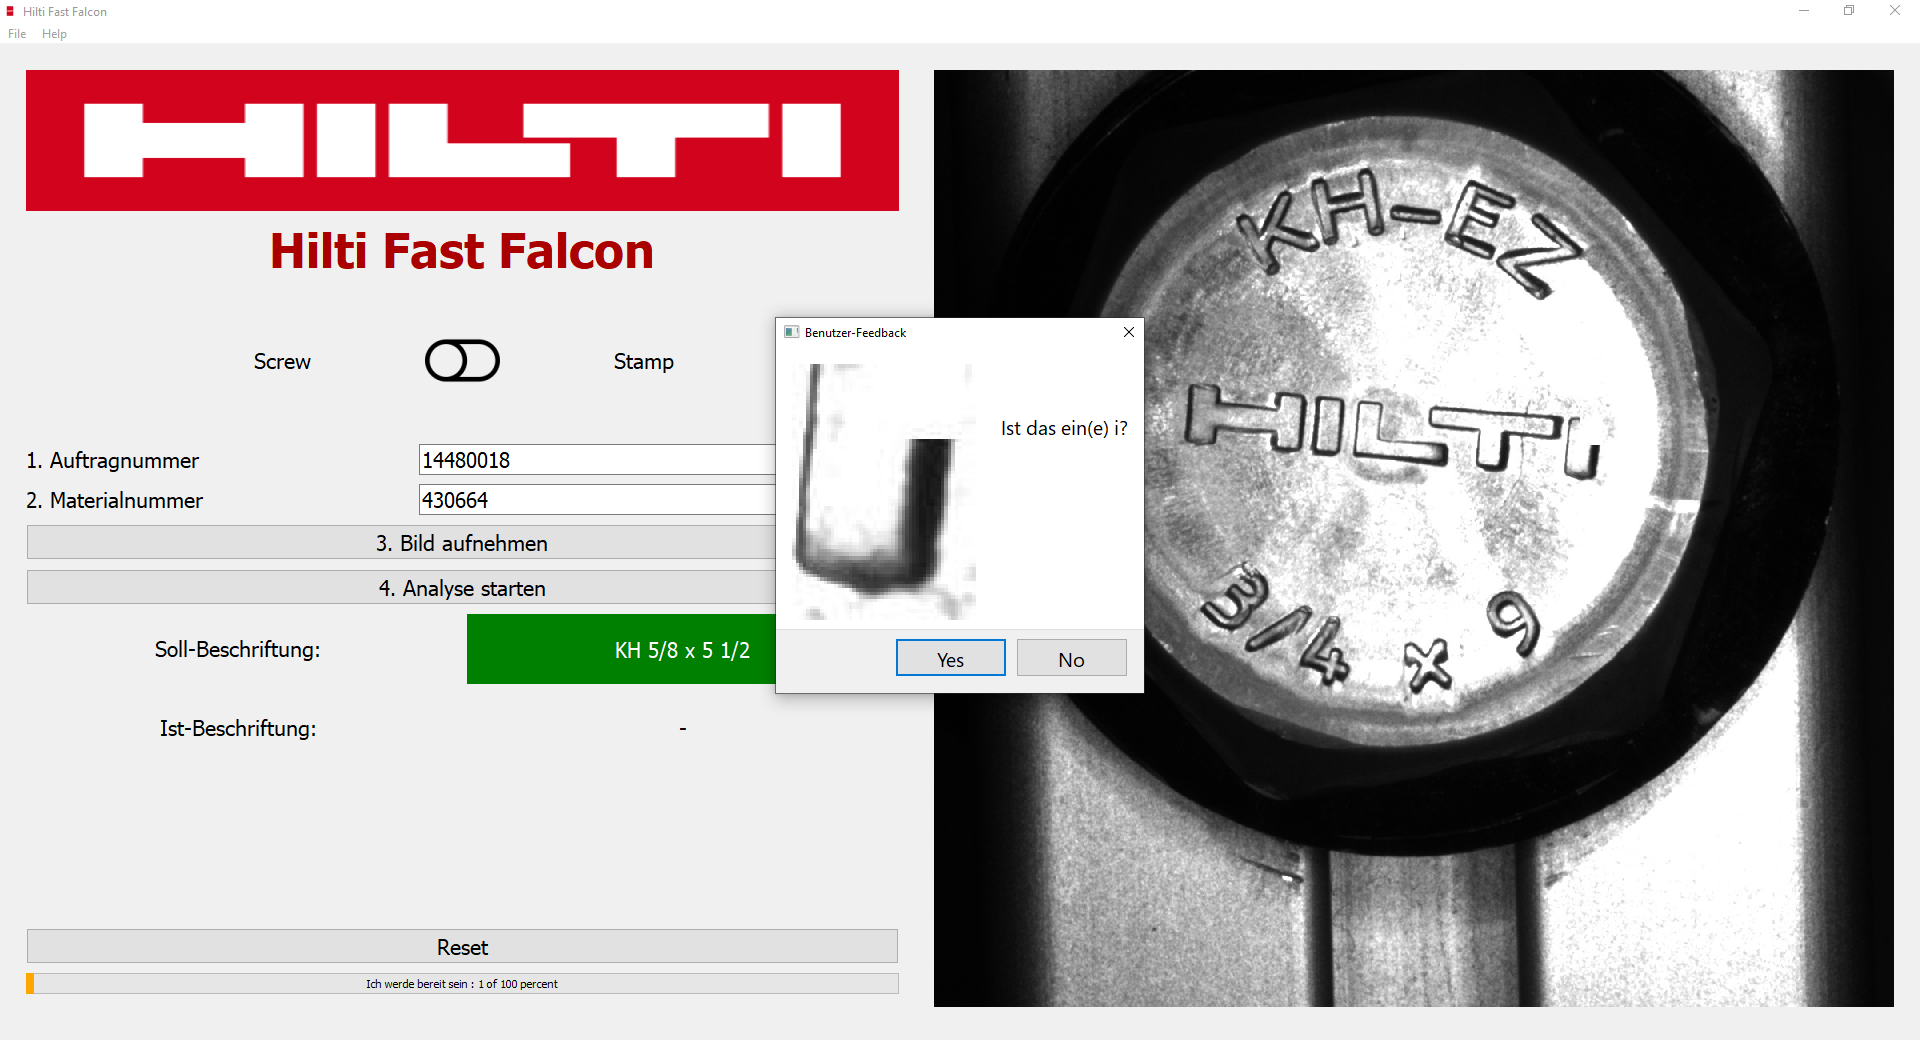
\includegraphics[width=\linewidth]{figure/alert.png}
  \subcaption{}
  \label{app_view_alt}
 \end{subfigure}
  \begin{subfigure}{0.6\textwidth}
  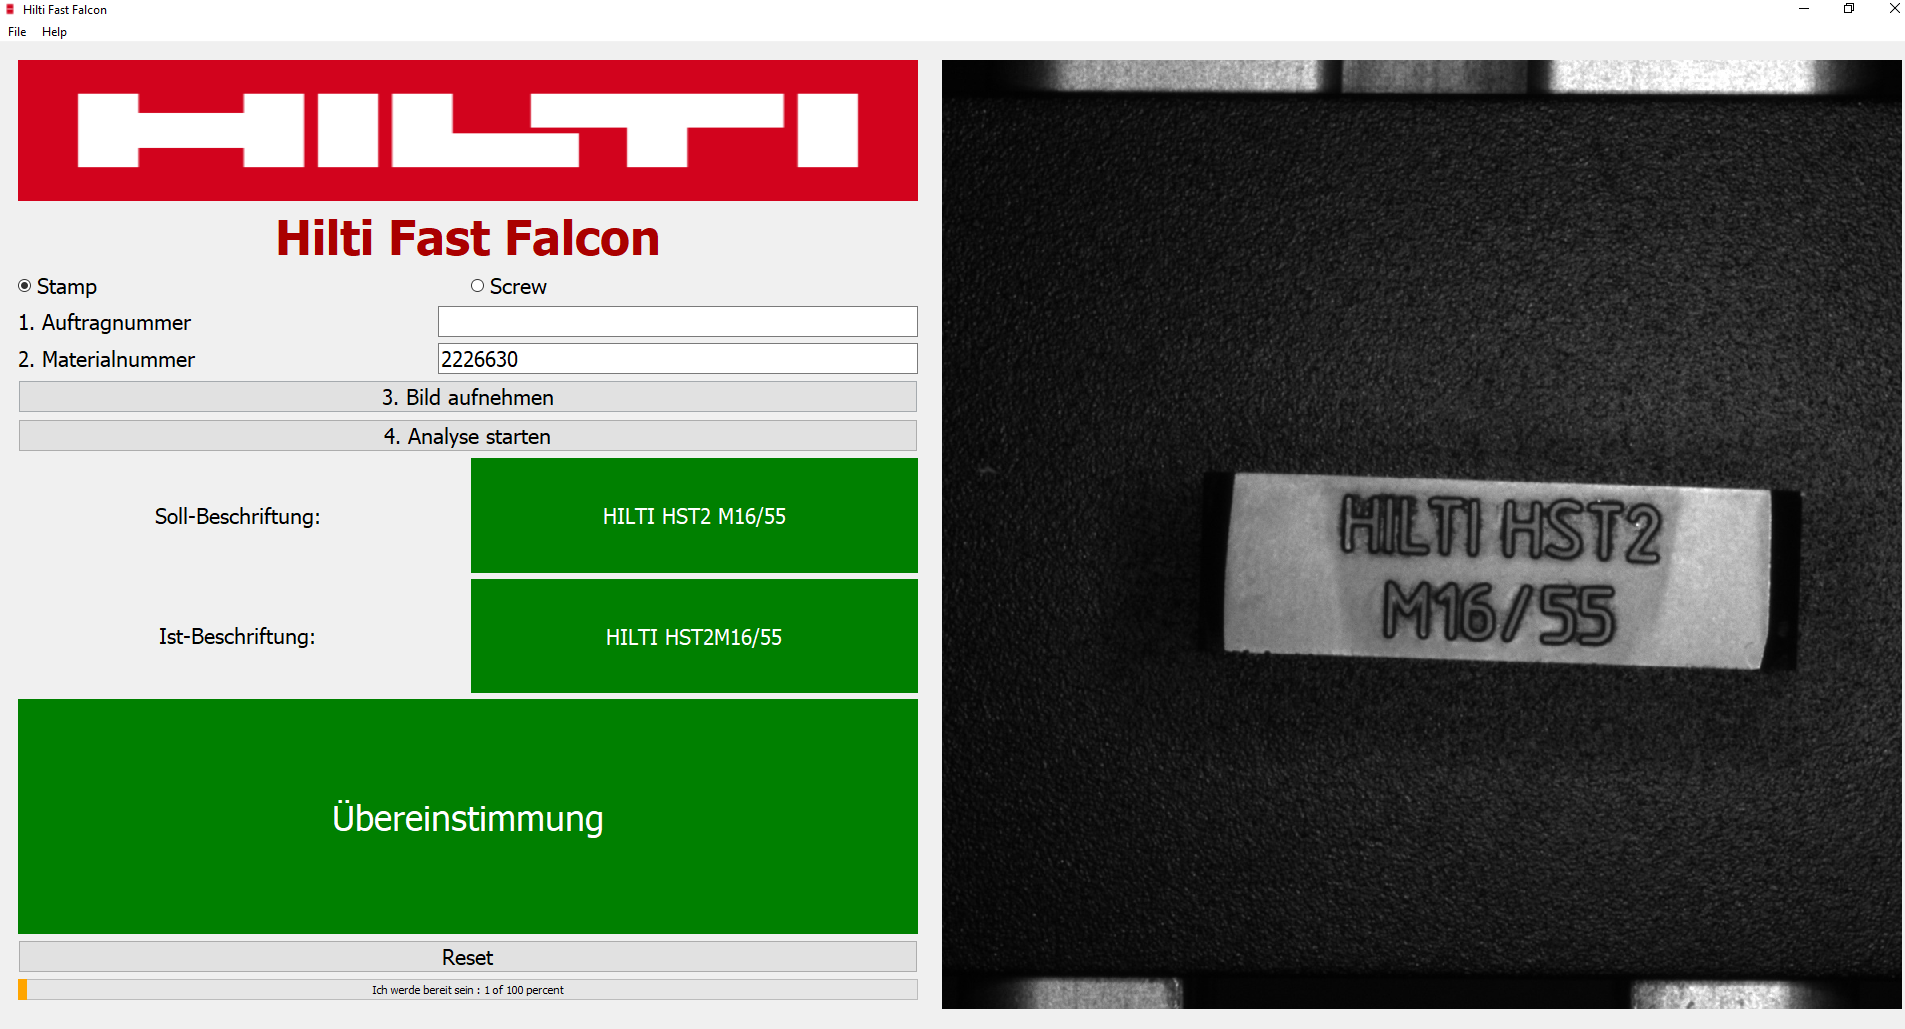
\includegraphics[width=\linewidth]{figure/SATMP_success.PNG}
  \subcaption{}
  \label{app_view_stamp_sucess}
 \end{subfigure}
 \begin{subfigure}{0.6\textwidth}
  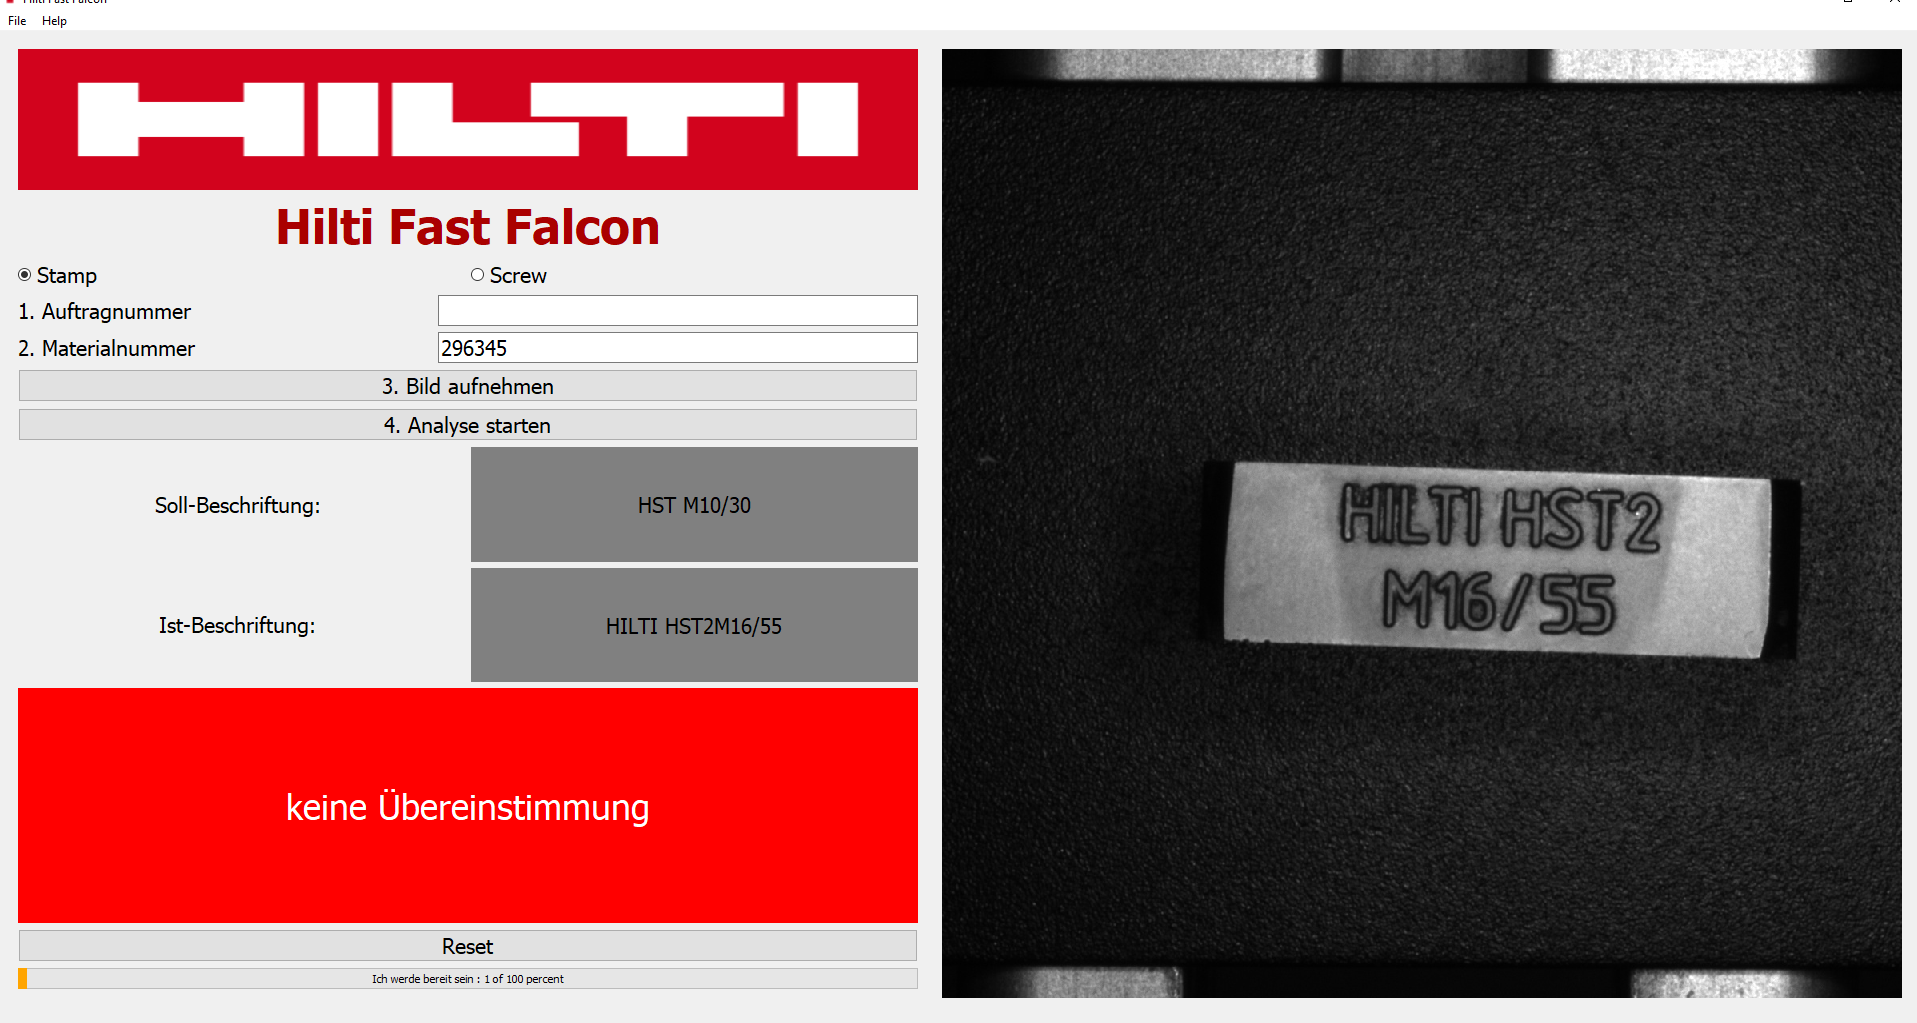
\includegraphics[width=\linewidth]{figure/SATMP_failure.PNG}
  \subcaption{}
  \label{app_view_stamp_echec}
 \end{subfigure}
 \caption{\textbf{Global views of the application} Alert display linked to the uncertainty of the algorithm with respect to the character shown in the pop-up windows. The user have to accept or reject the proposals before the results' be post-process. \textbf{B-C)} Analysis of a stamp picture that led respectively to a match (B) and to a mismatch (C) in respect with the expected label.}
 \label{APP_SUP}
\end{figure}%


\begin{landscape}
\begin{figure}[H]
 \centering
 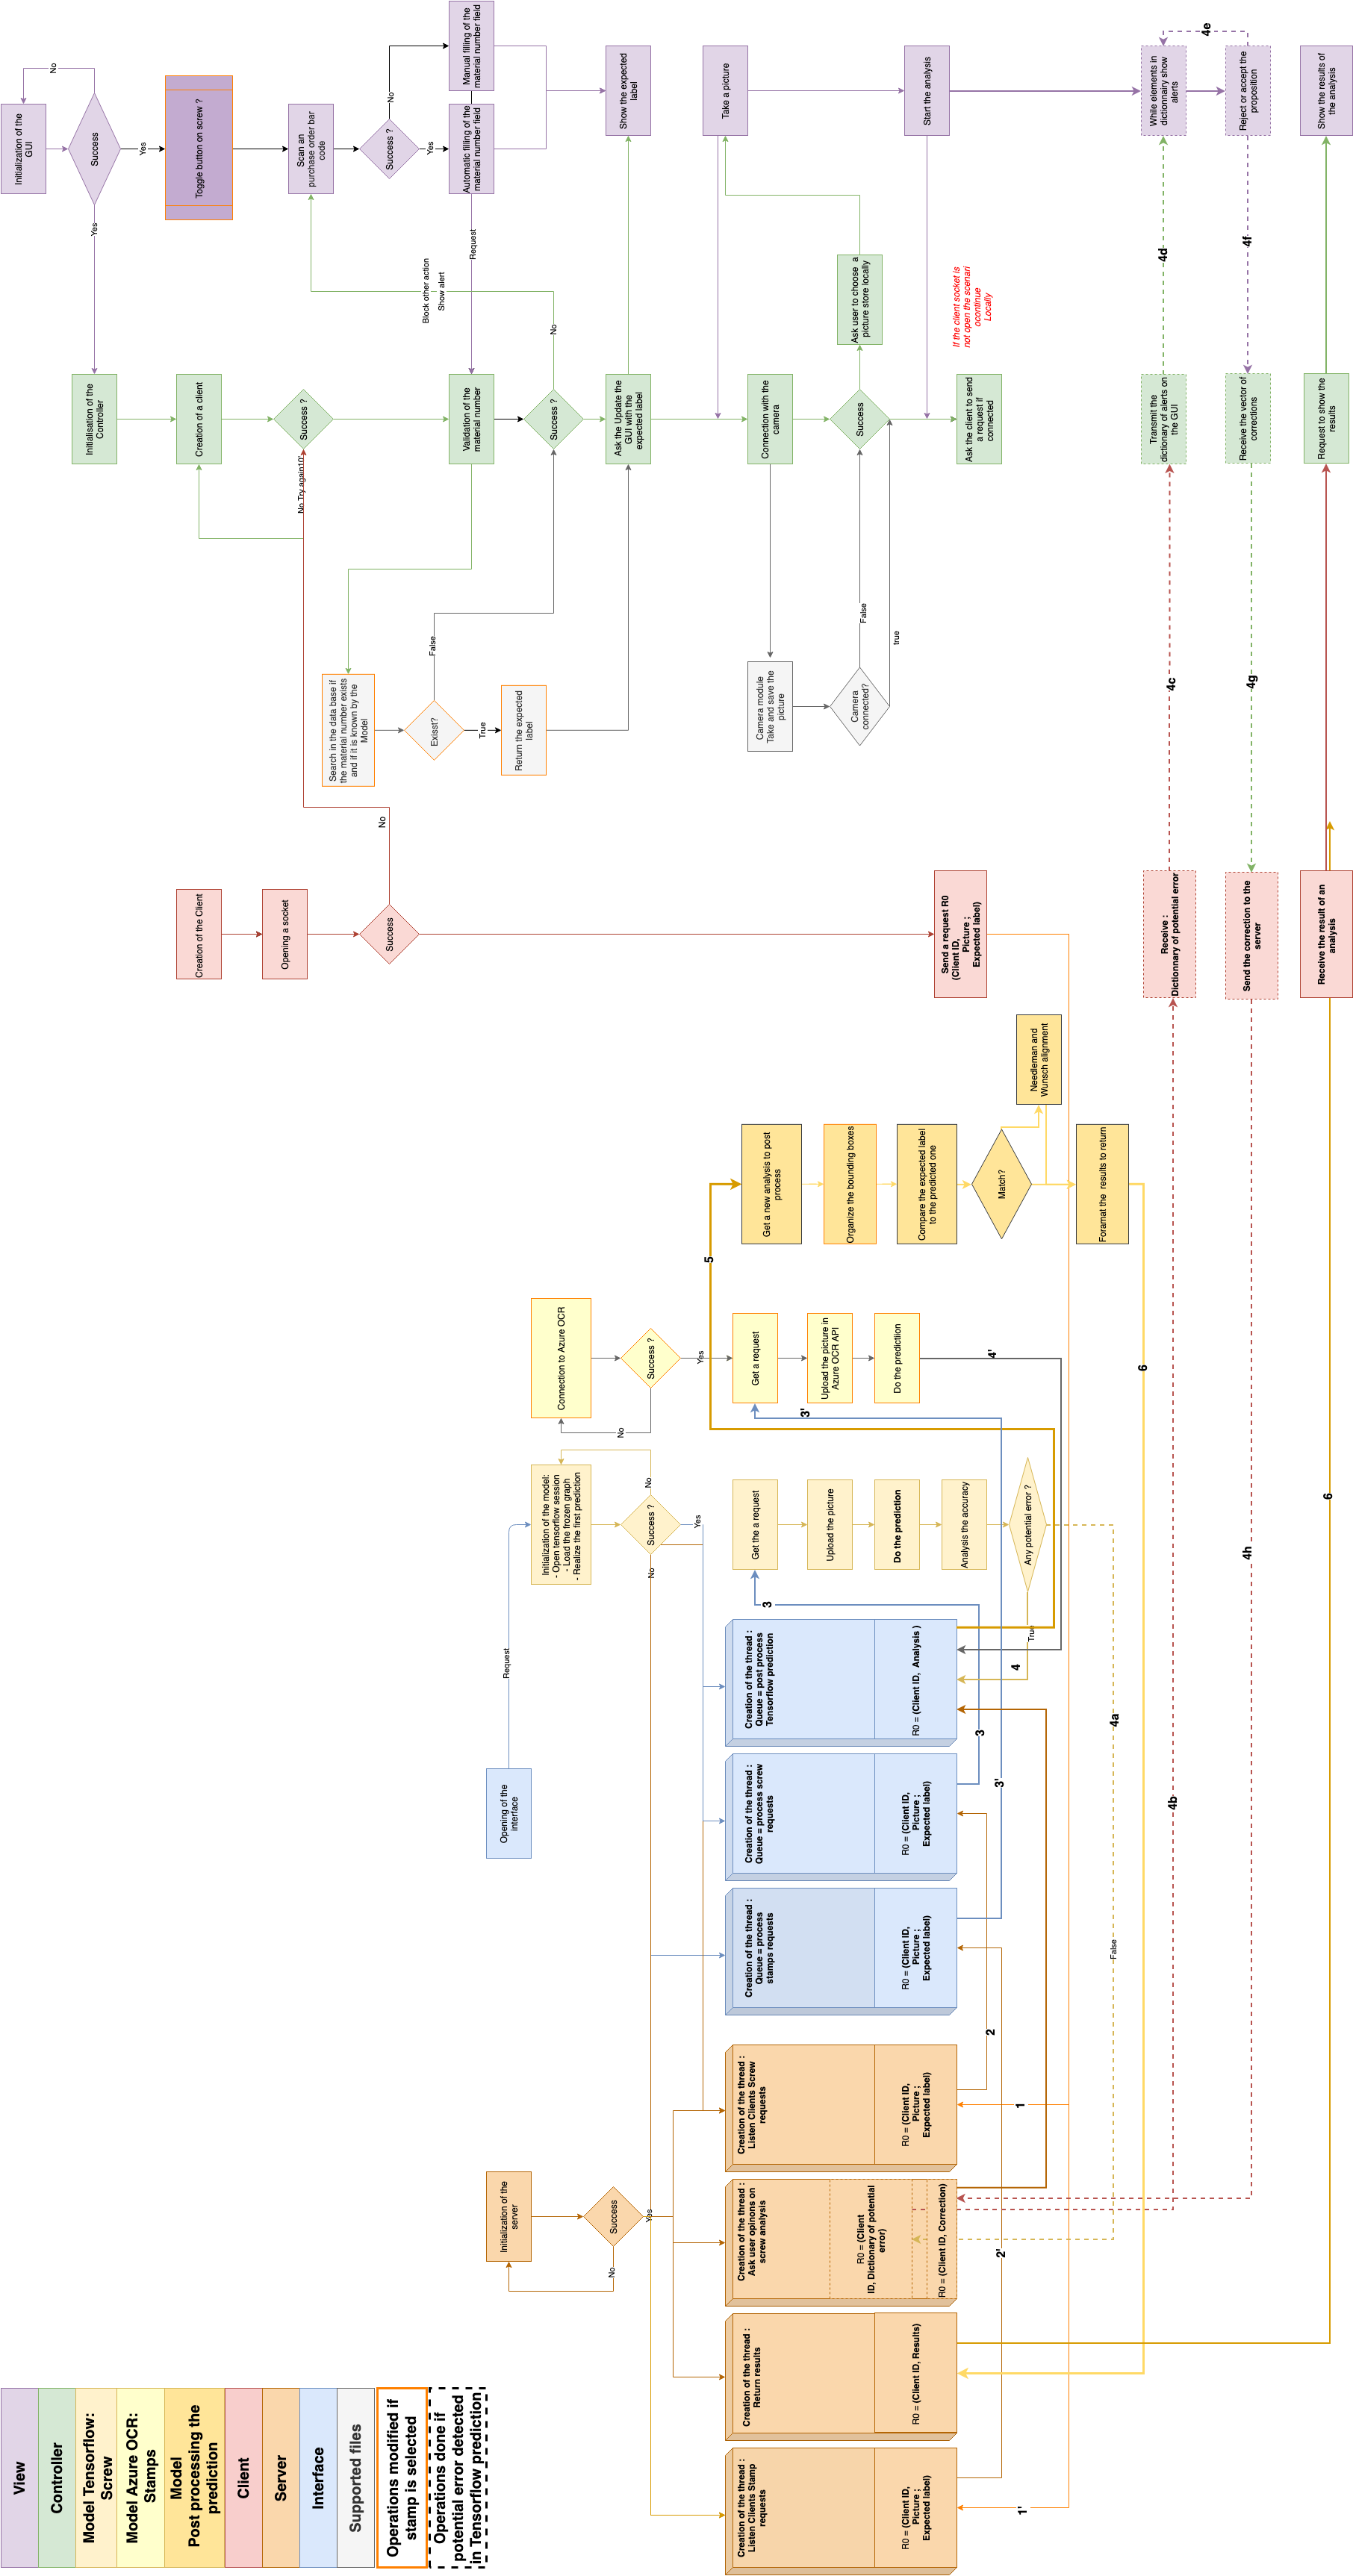
\includegraphics[angle=270,origin=c, width= 1\textwidth]{figure/MVC_SCA-3.png}
 \vspace{-2cm}
 \caption{\textbf{Detailed of the architecture \gls{MVC} Client Server} This diagram summarizes the interaction between the \gls{GUI} (violet boxes), the Controller (Green boxes) which is linked to the client if the server is connected (Red boxes) and the Model (yellow-orange boxes). User's requests are handle by the controller that through the client sends them to the server (Brown boxes), which is linked to the interface (blue boxes). The interface copes with requests' order and send them to the Model (Yellow-Orange boxes). The model is divided in three part one handles the request linked to the screw (Clear orange boxes), the other one the request corresponding to stamps (Clear yellow boxes). The results of the predictions are them post-processed (Dark yellow boxes), after to have been corrected by the user (doted line), if potential wrong bounding boxes have been predicted. To get a clearer view of this diagram please follow this link: \link{https://drive.google.com/file/d/1eJXbqYI5QIg-qIZLmVVT8fZpzbt9I5UG/view?usp=sharing} }
 \label{MVC_SCA}
\end{figure}
\end{landscape}

\\

\newpage
\section{Faster R-CNN Inception-v2-Resnet-v4 configuration}
\begin{multicols}{2}
\begin{Verbatim}[fontsize=\tiny]
model {
 faster_rcnn {
 num_classes: 20
 image_resizer {
  keep_aspect_ratio_resizer {
  min_dimension: 600
  max_dimension: 600
  }
 }
 feature_extractor {
  type: 'faster_rcnn_inception_resnet_v2'
  first_stage_features_stride: 8
 }
 first_stage_anchor_generator {
  grid_anchor_generator {
  scales: [0.25, 0.5, 1.0, 2.0]
  aspect_ratios: [0.5, 1.0, 2.0]
  height_stride: 8
  width_stride: 8
  }
 }
 first_stage_atrous_rate: 2
 first_stage_box_predictor_conv_hyperparams {
  op: CONV
  regularizer {
  l2_regularizer {
   weight: 0.0
  }
  }
  initializer {
  truncated_normal_initializer {
  stddev: 0.01
  }
  }
 }
 first_stage_nms_score_threshold: 0.0
 first_stage_nms_iou_threshold: 0.7
 first_stage_max_proposals: 300
 first_stage_localization_loss_weight: 2.0
 first_stage_objectness_loss_weight: 1.0
 initial_crop_size: 17
 maxpool_kernel_size: 1
 maxpool_stride: 1
 second_stage_box_predictor {
  mask_rcnn_box_predictor {
  use_dropout: false
  dropout_keep_probability: 1.0
  fc_hyperparams {
   op: FC
   regularizer {
   l2_regularizer {
    weight: 0.0
   }
   }
   initializer {
   variance_scaling_initializer {
    factor: 1.0
    uniform: true
    mode: FAN_AVG
   }
   }
  }
  }
 }
 second_stage_post_processing {
  batch_non_max_suppression {
  score_threshold: 0.0
  iou_threshold: 0.6
  max_detections_per_class: 100
  max_total_detections: 100
  }
  score_converter: SOFTMAX
 }
 second_stage_localization_loss_weight: 2.0
 second_stage_classification_loss_weight: 1.0
 }
}
train_config: {
 batch_size: 1
 batch_queue_capacity: 10
 num_batch_queue_threads: 10
 prefetch_queue_capacity:5
 optimizer {
 momentum_optimizer: {
  learning_rate: {
  manual_step_learning_rate {
   initial_learning_rate: 0.0003
   schedule {
   step: 900000
   learning_rate: .00003
   }
   schedule {
   step: 1200000
   learning_rate: .000003
   }
  }
  }
  momentum_optimizer_value: 0.9
 }
 use_moving_average: false
 }
 gradient_clipping_by_norm: 10.0
 fine_tune_checkpoint: "PATH/TO/THE/LAST/FROZEN-GRAPH"
 from_detection_checkpoint: true
 num_steps: 200000
 data_augmentation_options {
 random_horizontal_flip {
 }
 }
}
train_input_reader: {
 tf_record_input_reader {
 input_path: "PATH/TO/TRAIN.RECORD/FILE"
 }
 label_map_path: "PATH/TO/LABELMAP.pbtxt"
 queue_capacity: 2
 min_after_dequeue: 1
 num_readers: 1
}
eval_config: {
 metrics_set: "coco_detection_metrics"
 num_examples: 33
 num_visualizations: 10
}
eval_input_reader: {
 tf_record_input_reader {
 input_path: "PATH/TO/VAL.RECORD/FILE"
 }
 label_map_path: "PATH/TO/LABELMAP.pbtxt"
 shuffle: false
 num_readers: 1
 queue_capacity: 1
}
\end{Verbatim}
\label{config}
\end{multicols}




%---------------------------------------------------------------------------------




 \end{document}


